\noindent\textbf{Team Control Number:} \# 2625838\\
\textbf{Problem:} C\\

\vspace{0.1em}
\subsection*{AI Tools Used}
\begin{table}[h!]
\centering
\small
\setlength{\tabcolsep}{6pt}
\renewcommand{\arraystretch}{1.15}
\begin{tabular}{|p{3.2cm}|p{3.2cm}|p{8.2cm}|}
\hline
\textbf{AI Tool} & \textbf{Version / Model} & \textbf{Primary Purpose} \\
\hline
OpenAI ChatGPT  & GPT-5.2 &
Language polishing, structural refinement, and clarification of written explanations \\
OpenAI ChatGPT & GPT-5.2 &
Brainstorming ideas for modeling approaches, algorithm designs, and solution strategies \\
OpenAI ChatGPT & GPT-5.2 &
Generating preliminary code drafts for data processing, graph producing and simulation, later reviewed and modified by the team \\
OpenAI ChatGPT & GPT-5.2 &
Synthesis of the explanatory documents, work orders, template tickets for internal team Delivery \\
OpenAI ChatGPT & GPT-5.2 &
Giving Advice on engineered Document Management and Version Control best practices \\
Github Copilot & \center{---} & Enhance productivity while maintaining full control over the code quality and integrity\\
\hline
\end{tabular}
\end{table}

\subsection*{Query/Response Record}
Click \textbf{ChatGPT Query \#} to view the full input and output records on GitHub. Screenshots of the outputs are provided below for reference.
\textbf{\href{https://github.com/charles65536/model2026-2/blob/main/report_on_use_of_ai/chatgpt_1_output.md}{ChatGPT Query 1:}}\\
\textbf{Input:}
We just inished our setting of \textit{dynamic\_files}, please refer to the \textit{first\_stage\_modeling.md} and \textit{context\_pack\_for\_ai.md} in our repository, 
and search for authorative and highly credible supporting literature on topics of convex optimization/scalable solving, underdetermined inversion/regularization, ranking/rule differences, compositional data, simulation and sensitivity\\
\textbf{Output:}
\begin{figure}[H]
  \centering
  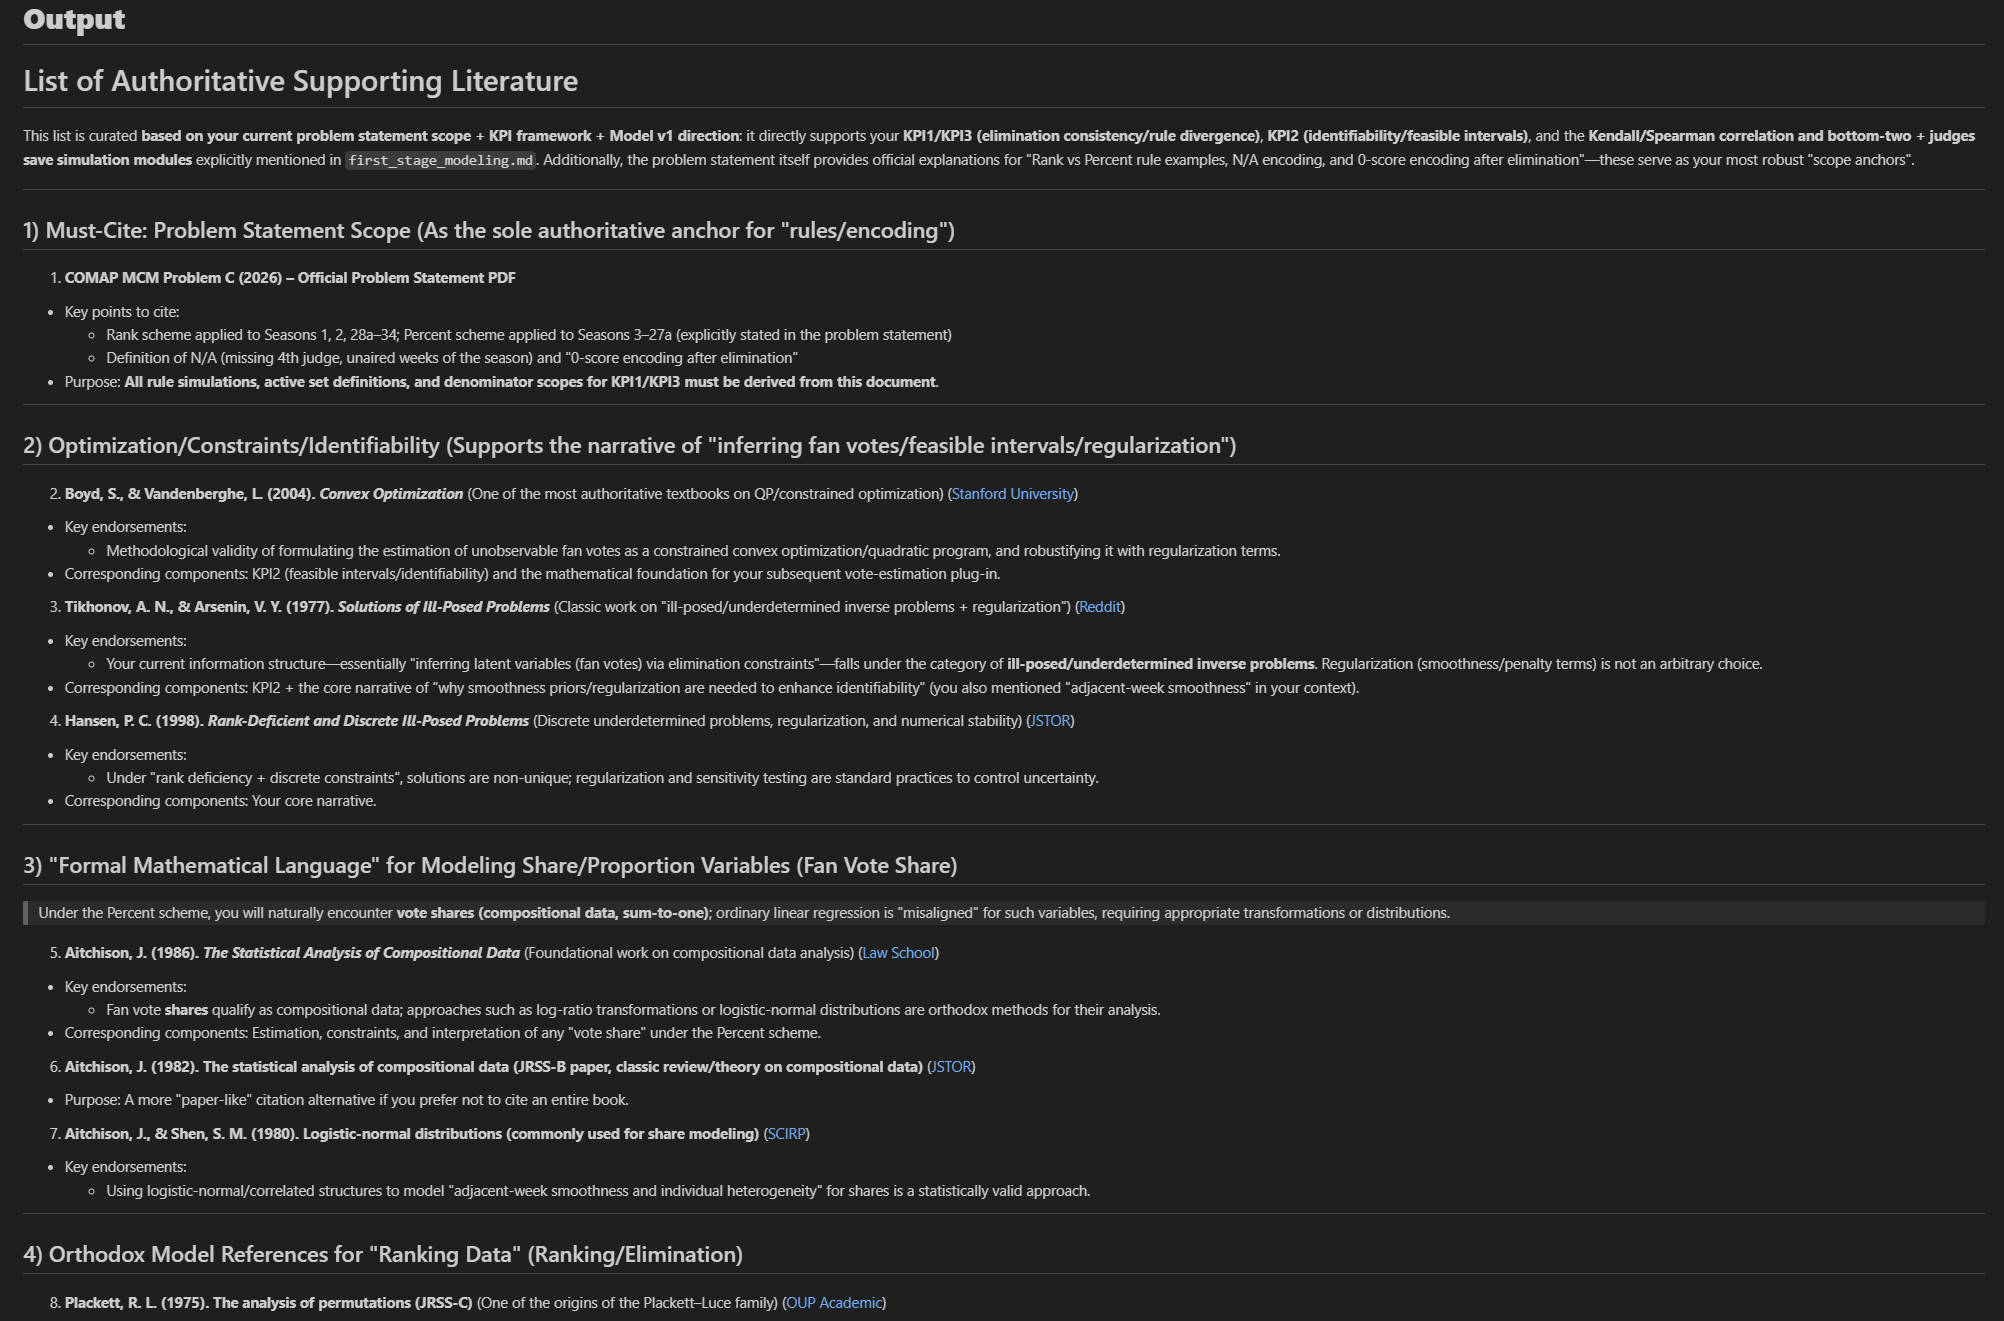
\includegraphics[width=0.9\linewidth]{report_on_use_of_ai/pho/1_1.png}
  \caption{ChatGPT Query 1 Output Screenshot}
  \label{fig:chatgpt_query_1_output}
\end{figure}
\begin{figure}[H]
  \centering
  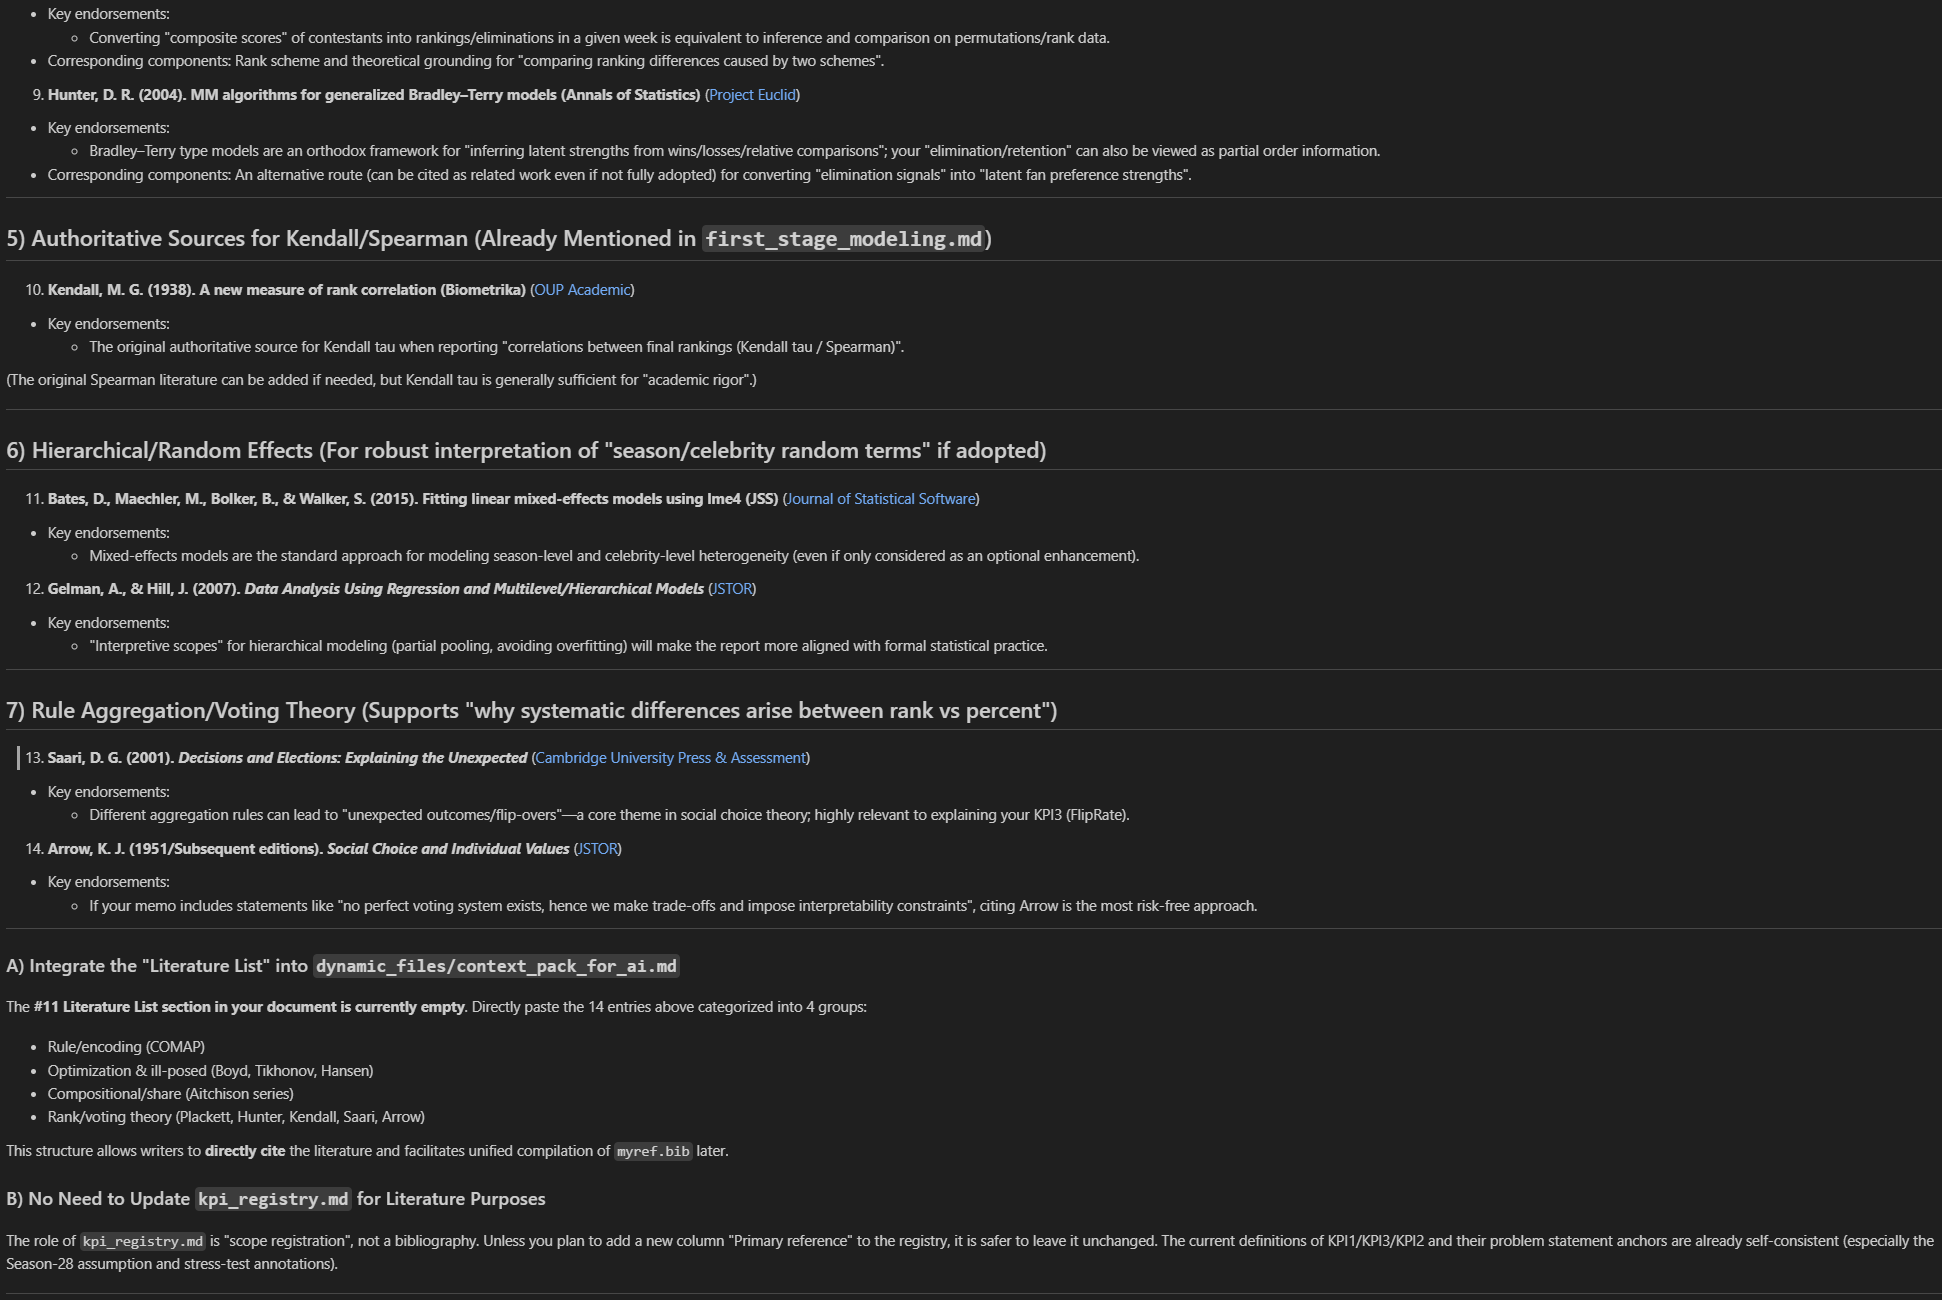
\includegraphics[width=0.9\linewidth]{report_on_use_of_ai/pho/1_2.png}
  \caption{ChatGPT Query 1 Output Screenshot (Continued)}
  \label{fig:chatgpt_query_1_output_2} 
\end{figure}

\textbf{\href{https://github.com/charles65536/model2026-2/blob/main/report_on_use_of_ai/chatgpt_2_input_and_output.md}{ChatGPT Query 2:}}\\
\begin{figure}[H]
  \centering
  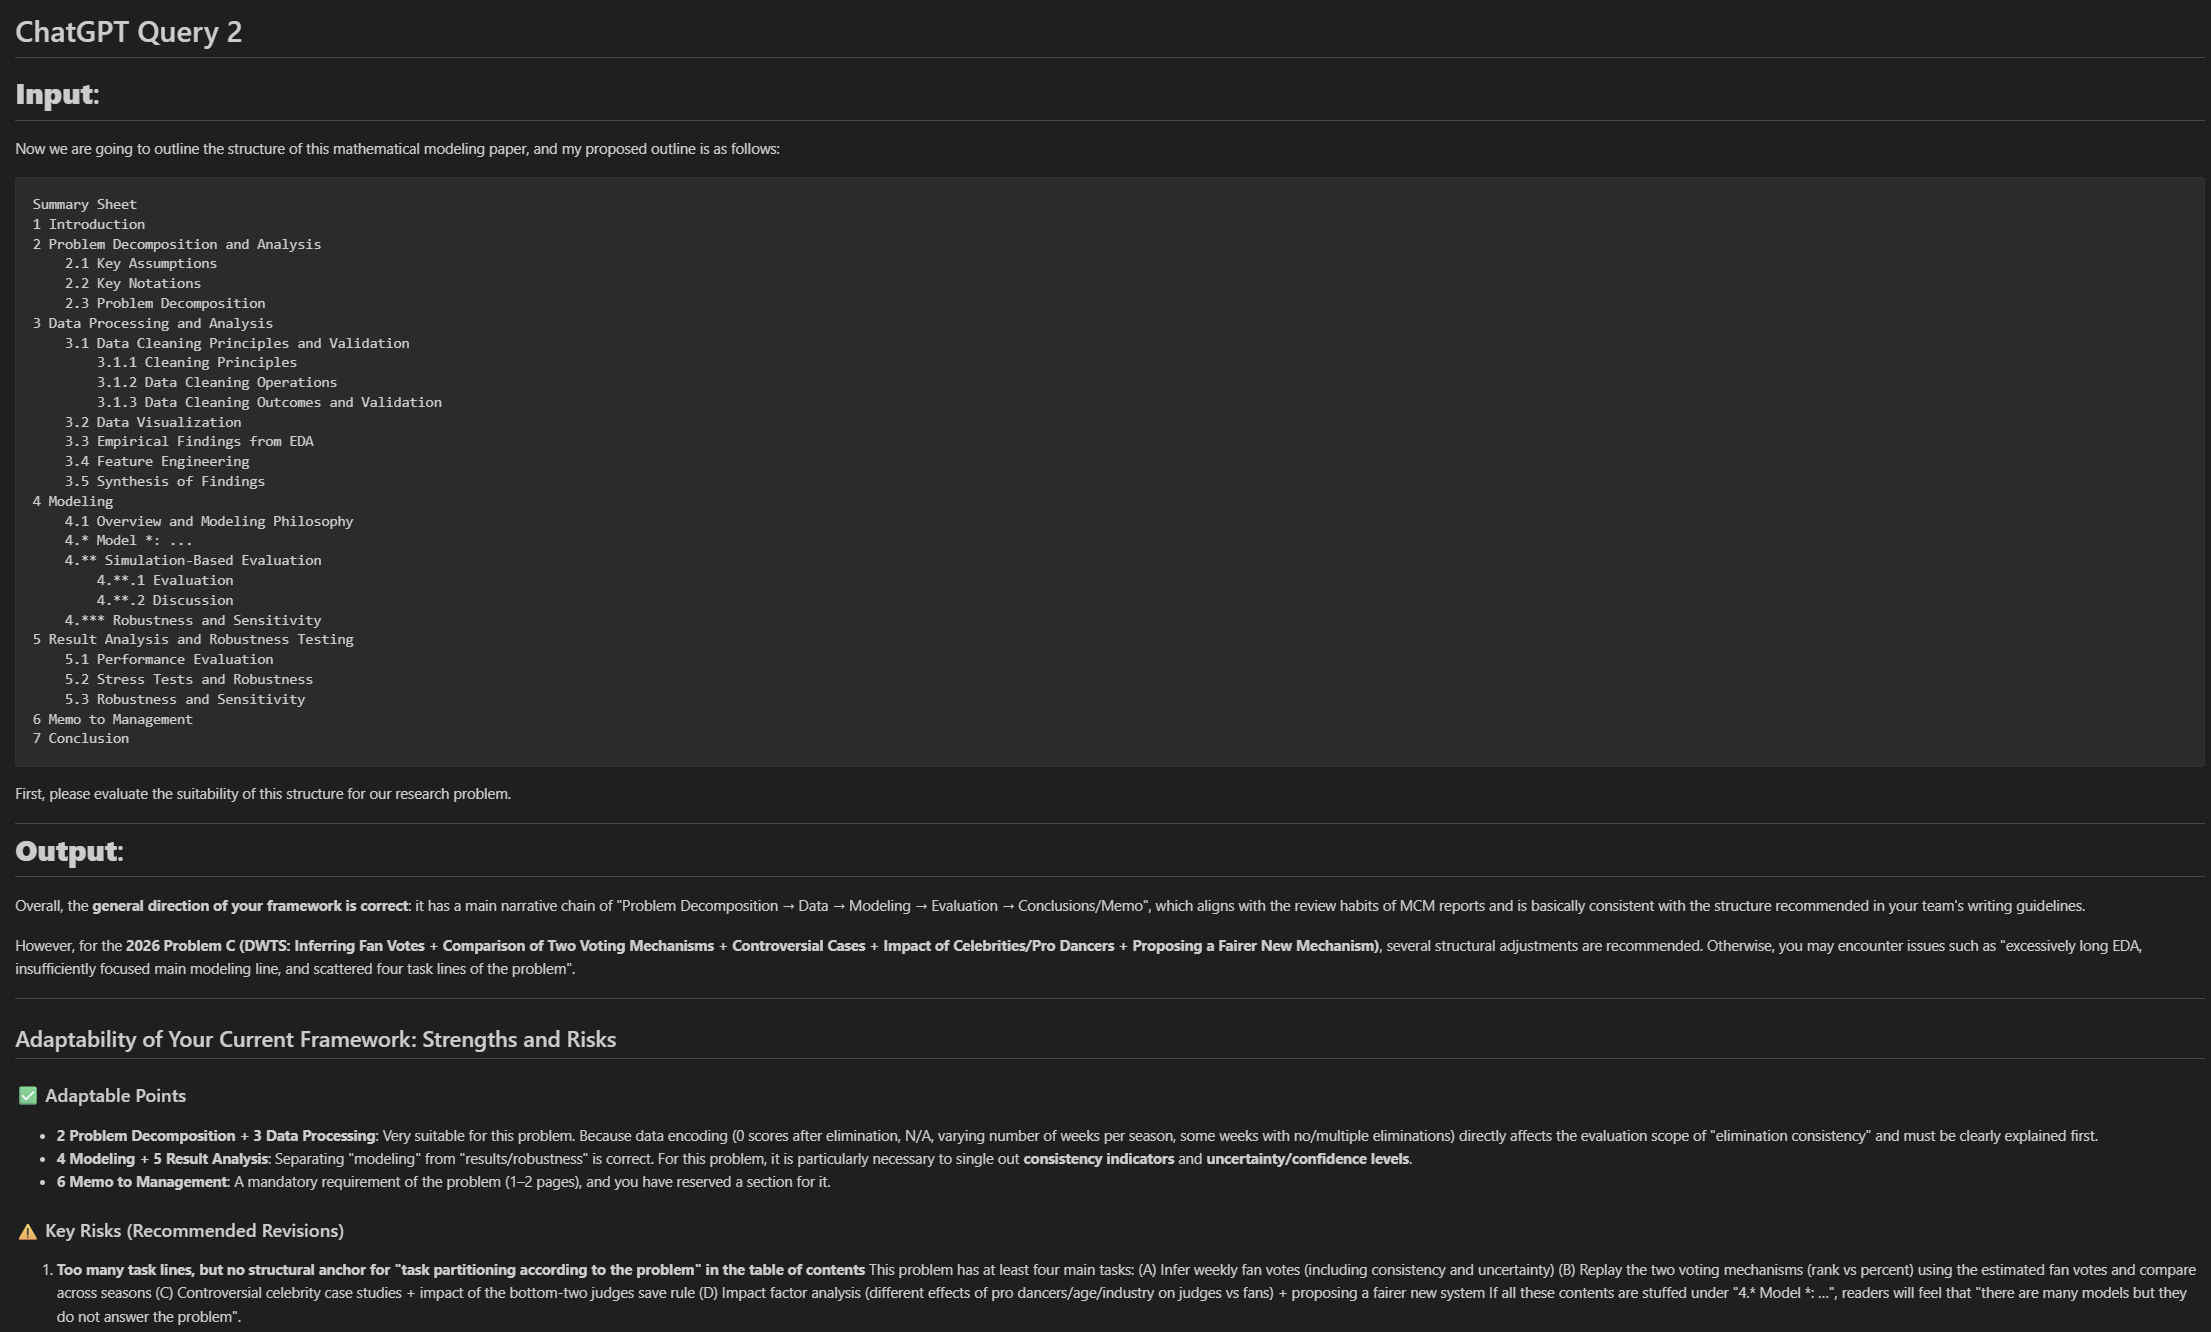
\includegraphics[width=0.9\linewidth]{report_on_use_of_ai/pho/2_1.png}
  \caption{ChatGPT Query 2 Output Screenshot}
  \label{fig:chatgpt_query_2_output}
\end{figure}
\begin{figure}[H]
  \centering
  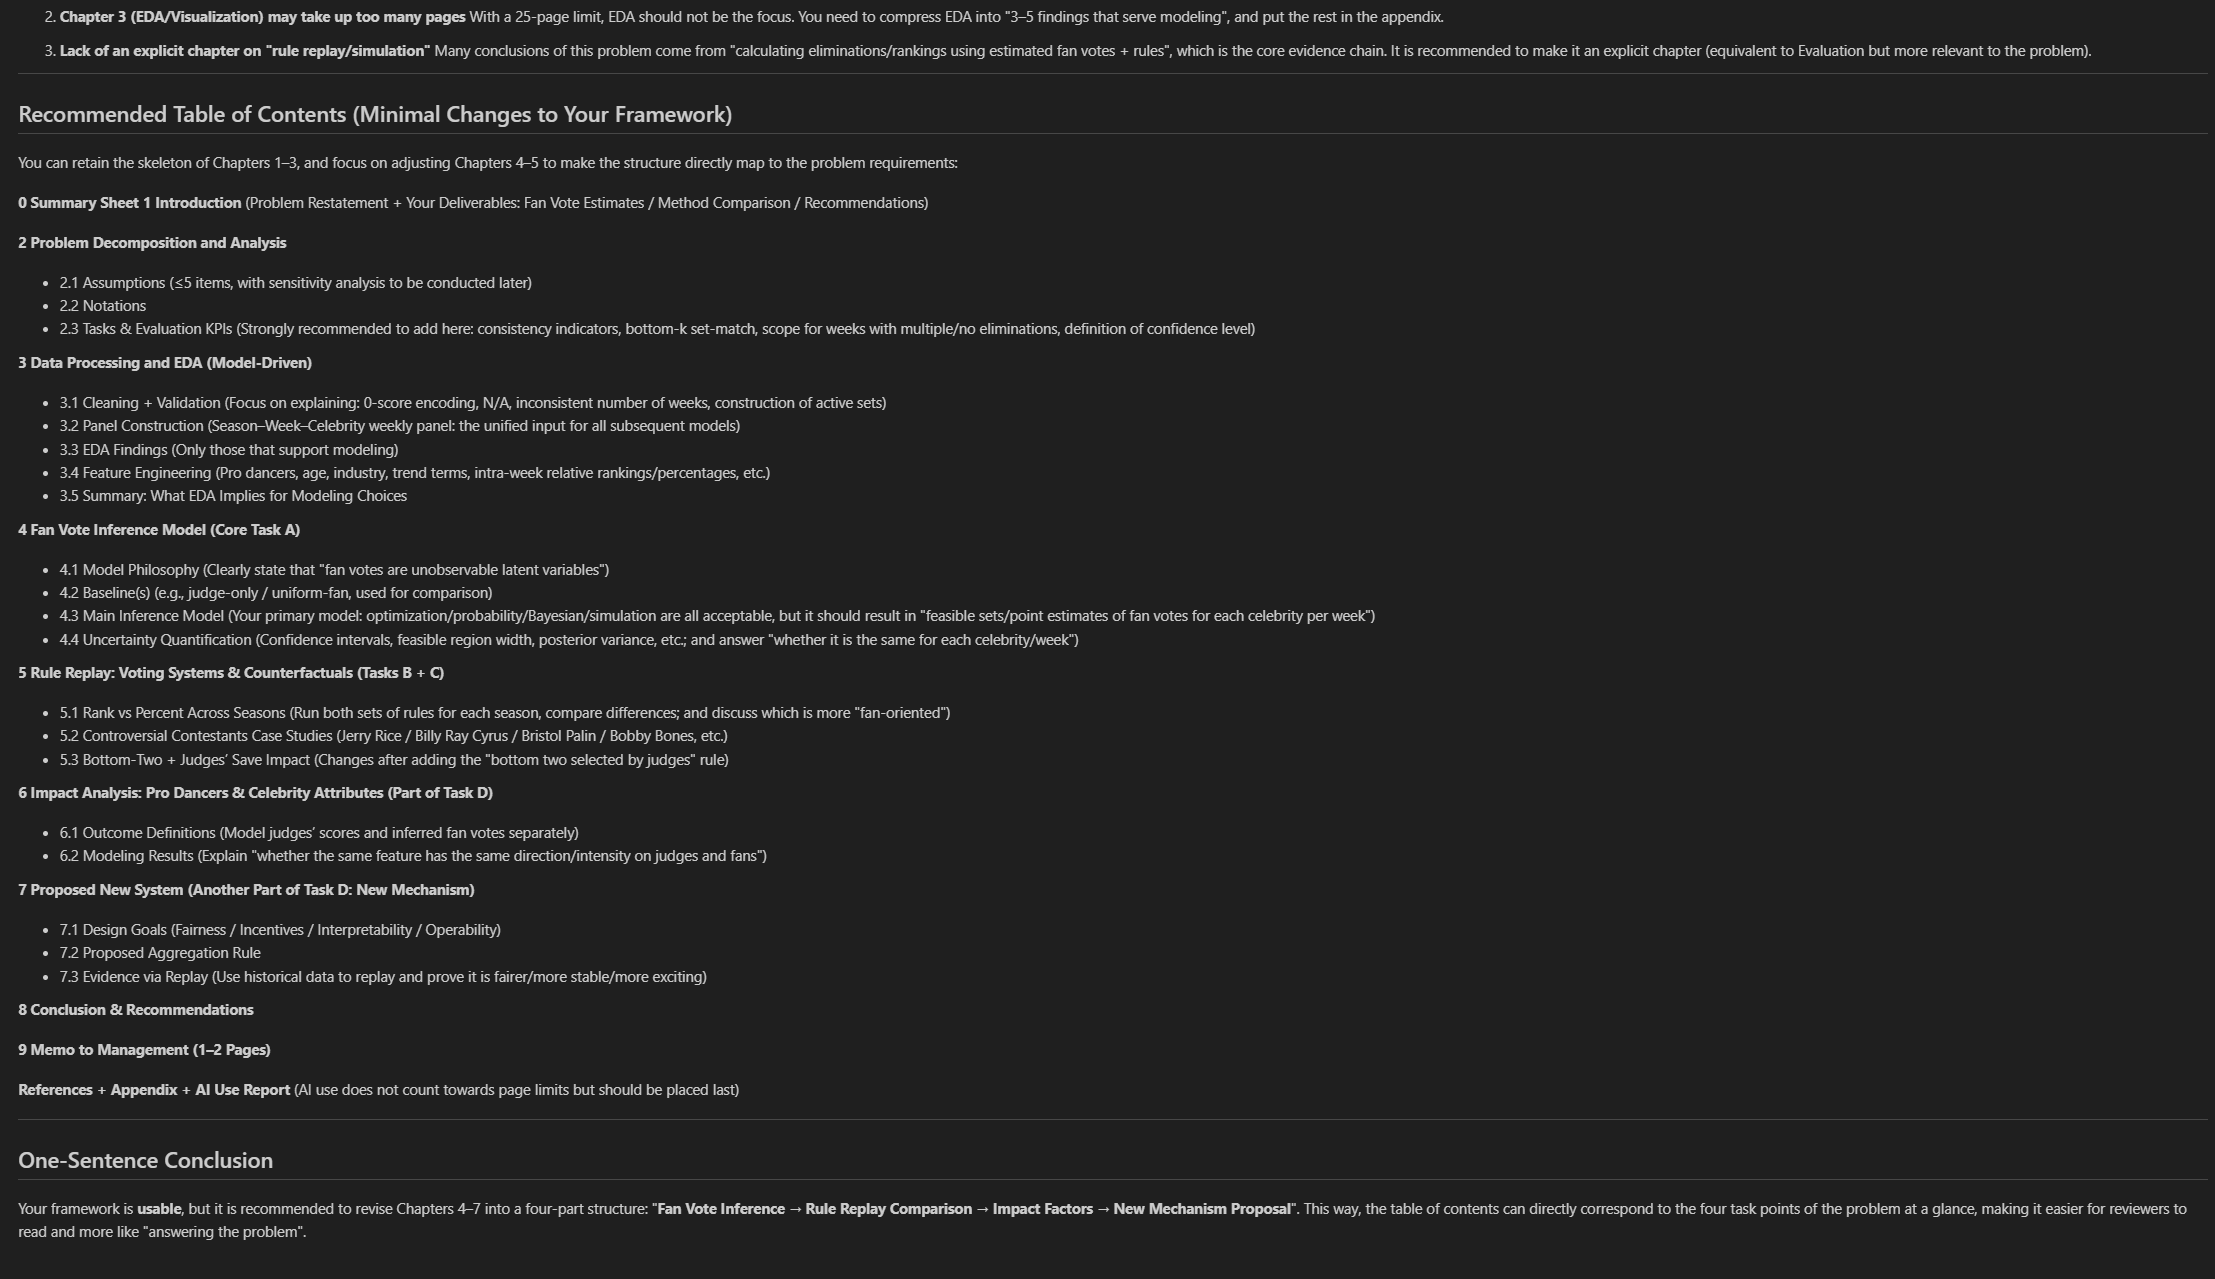
\includegraphics[width=0.9\linewidth]{report_on_use_of_ai/pho/2_2.png}
  \caption{ChatGPT Query 2 Output Screenshot (Continued)}
  \label{fig:chatgpt_query_2_output_2}
\end{figure}

\textbf{\href{https://github.com/charles65536/model2026-2/blob/main/report_on_use_of_ai/chatgpt_3_input_and_output.md}{ChatGPT Query 3:}}\\
\textbf{Input:}
\begin{figure}[H]
  \centering
  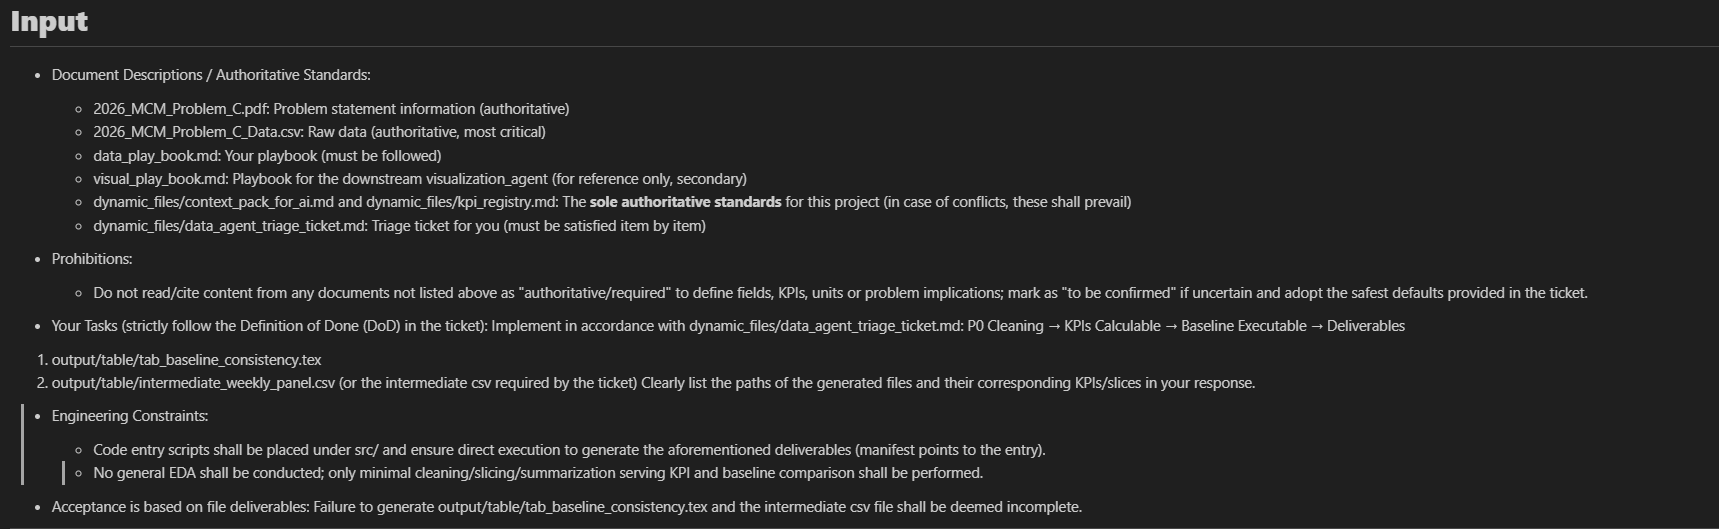
\includegraphics[width=0.9\linewidth]{report_on_use_of_ai/pho/3_1.png}
  \caption{ChatGPT Query 3 Input Screenshot}
  \label{fig:chatgpt_query_3_input}
\end{figure}
\textbf{Output:}
\begin{figure}[H]
  \centering
  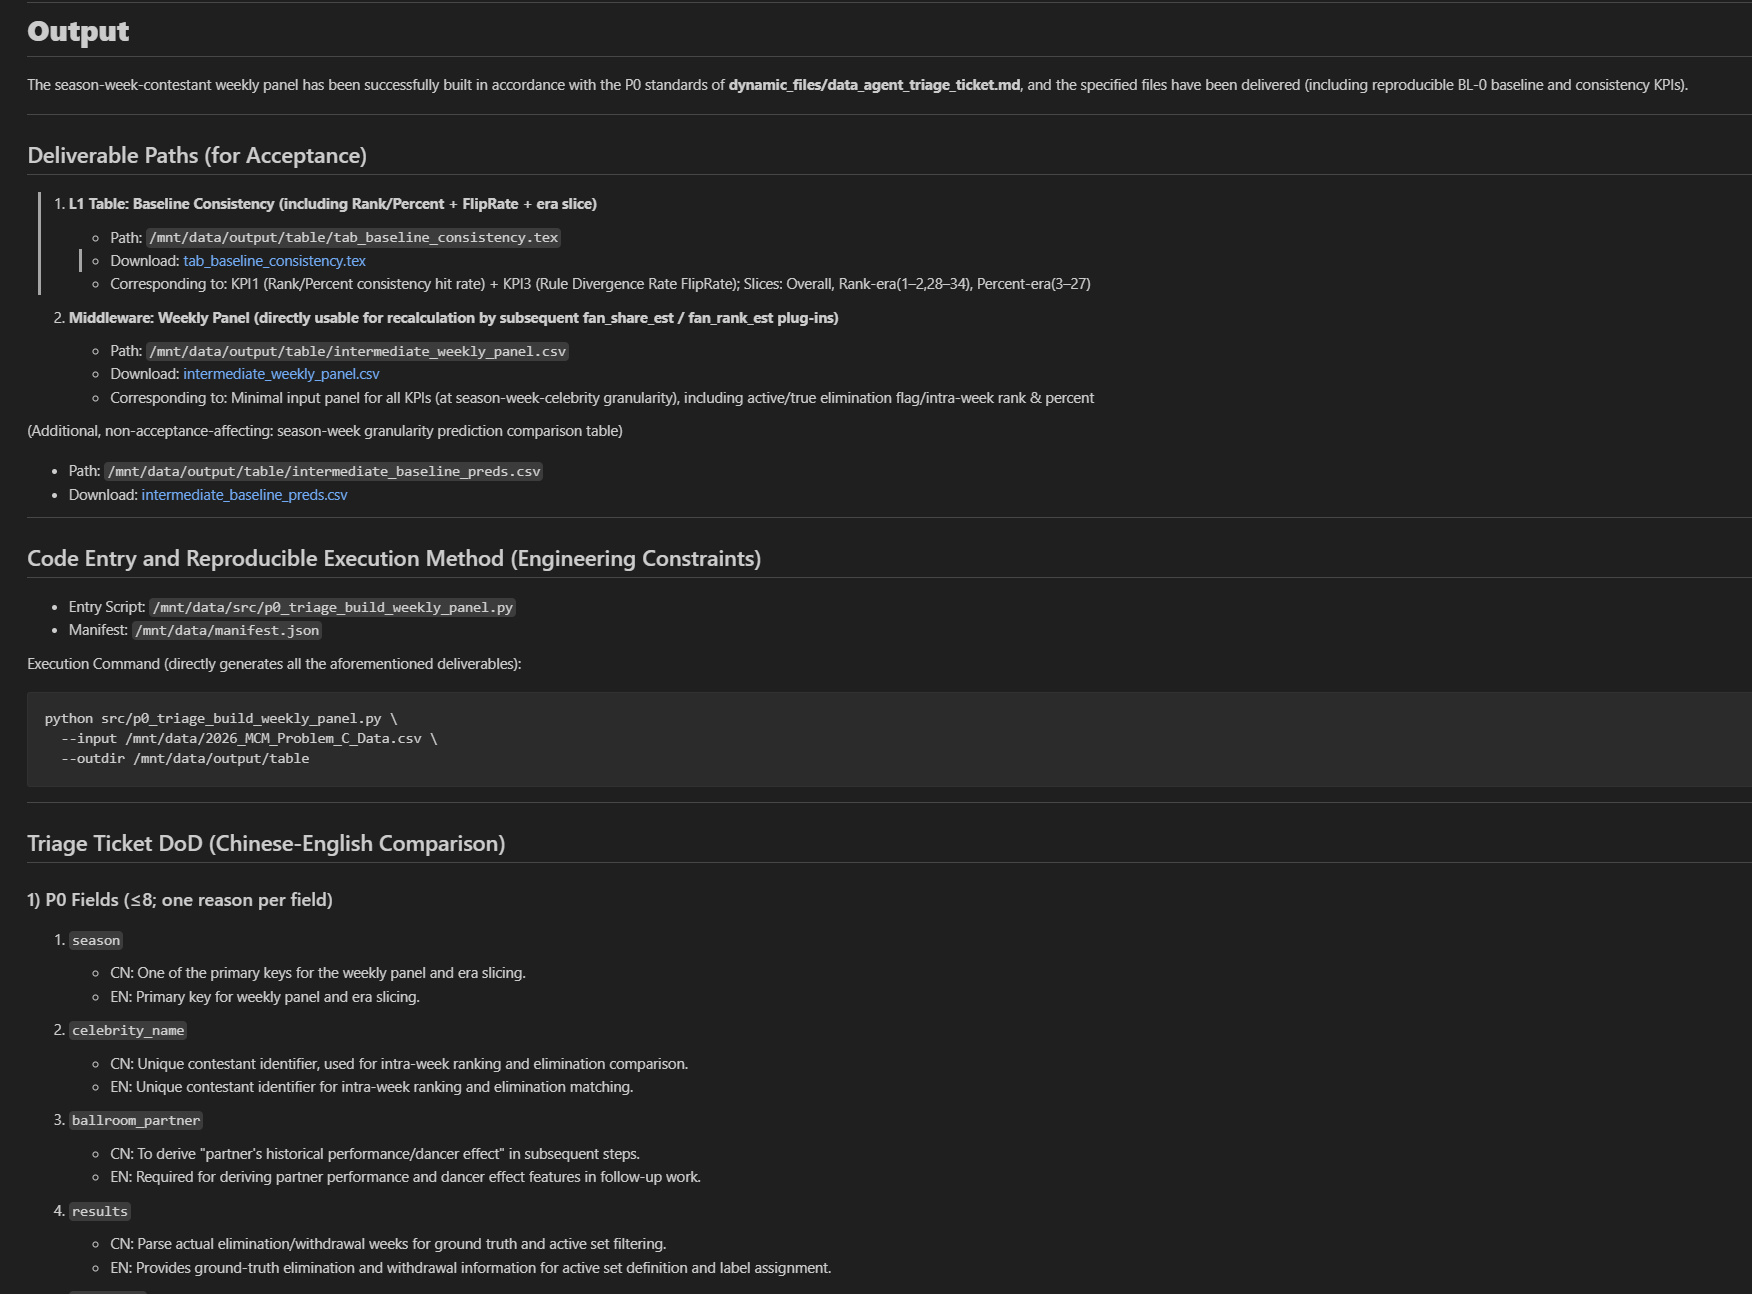
\includegraphics[width=0.9\linewidth]{report_on_use_of_ai/pho/3_2.png}
  \caption{ChatGPT Query 3 Output Screenshot}
  \label{fig:chatgpt_query_3_output}
\end{figure}
\begin{figure}[H]
  \centering
  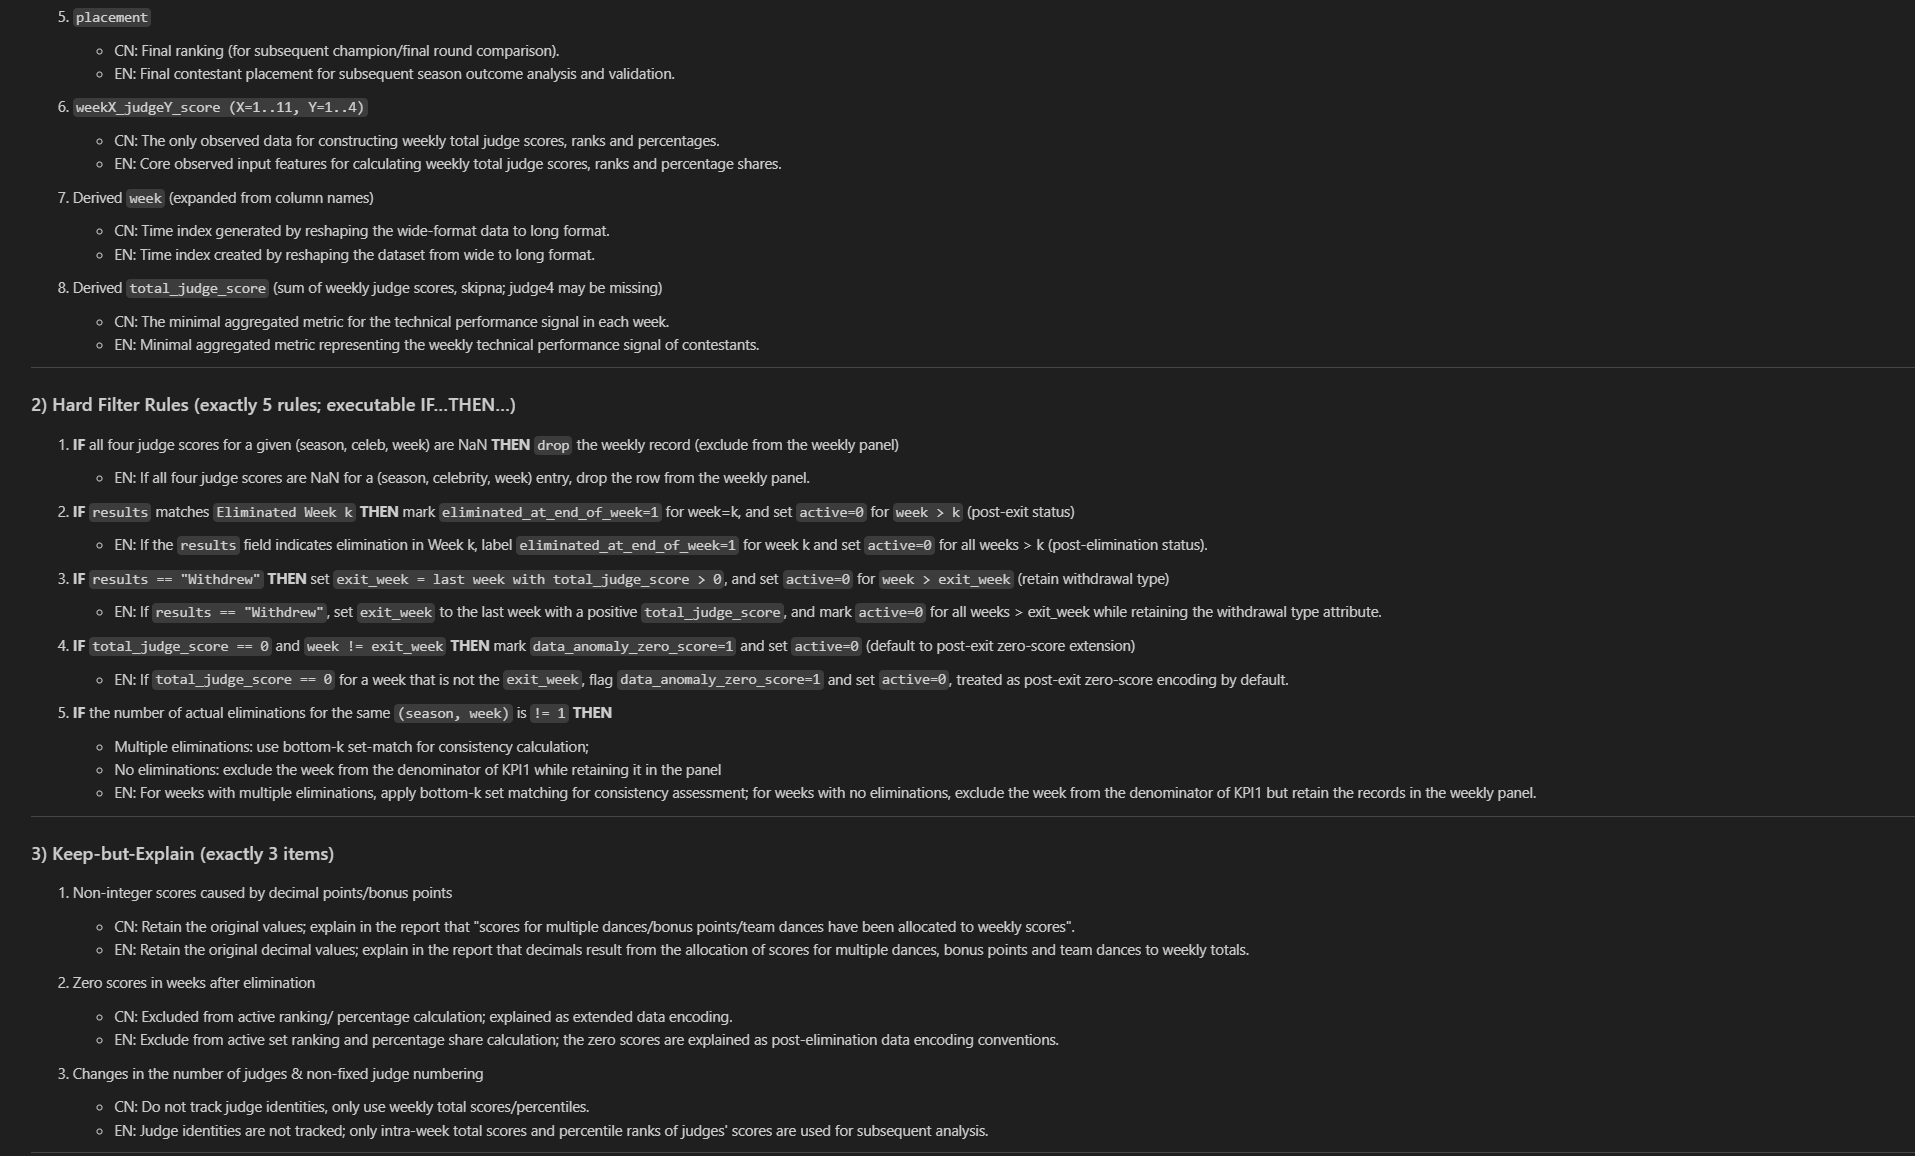
\includegraphics[width=0.9\linewidth]{report_on_use_of_ai/pho/3_3.png}
  \caption{ChatGPT Query 3 Output Screenshot (Continued)}
  \label{fig:chatgpt_query_3_output_2}
\end{figure}
\begin{figure}[H]
  \centering
  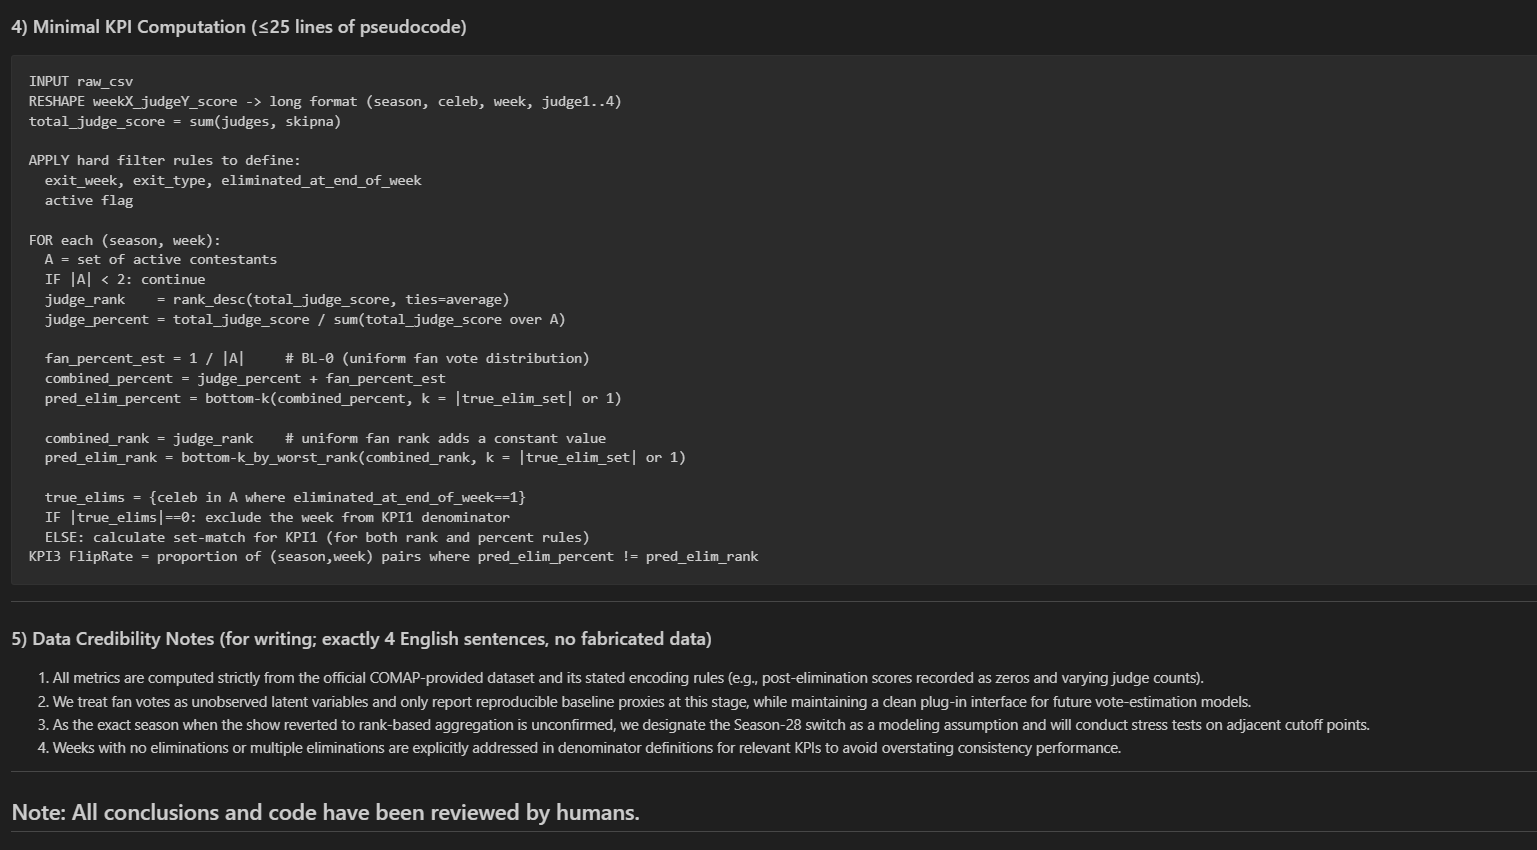
\includegraphics[width=0.9\linewidth]{report_on_use_of_ai/pho/3_4.png}
  \caption{ChatGPT Query 3 Output Screenshot (Continued)}
  \label{fig:chatgpt_query_3_output_3}
\end{figure}




\textbf{\href{https://github.com/charles65536/model2026-2/blob/main/report_on_use_of_ai/chatgpt_4_input_and_output.md}{ChatGPT Query 4:}}\\
\textbf{Input:}
Wait, why is the generated .pdf file completely unchanged? Could there be an issue with how we implemented the rules? Also, where in the code you provided do we need to modify the paths for importing and exporting files?\\
\textbf{Output:}
\begin{figure}[H]
  \centering
  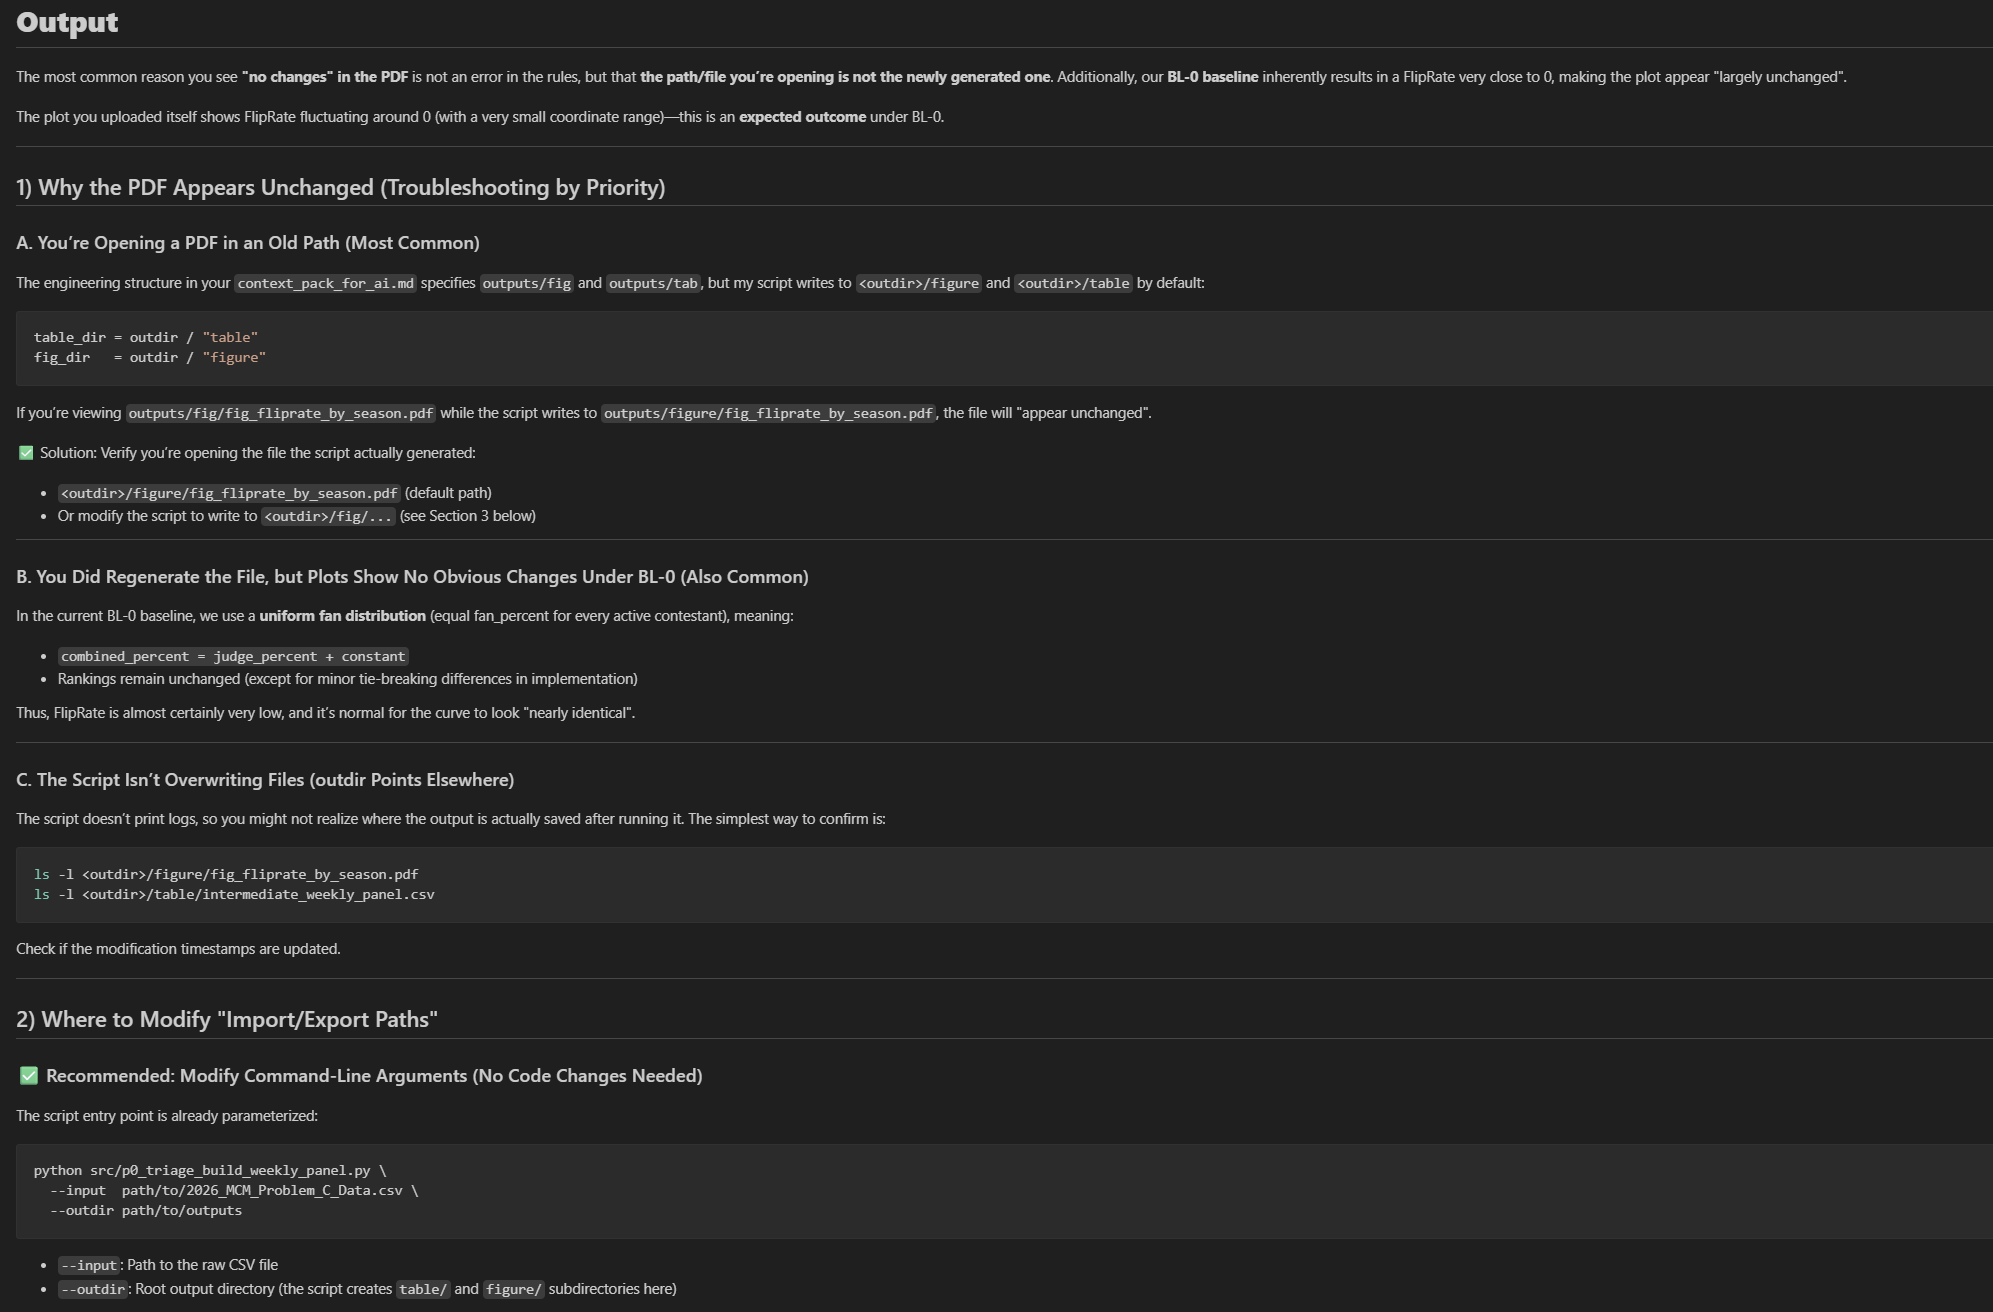
\includegraphics[width=0.9\linewidth]{report_on_use_of_ai/pho/4_1.png}
  \caption{ChatGPT Query 4 Output Screenshot}
  \label{fig:chatgpt_query_4_output}
\end{figure}
\begin{figure}[H]
  \centering
  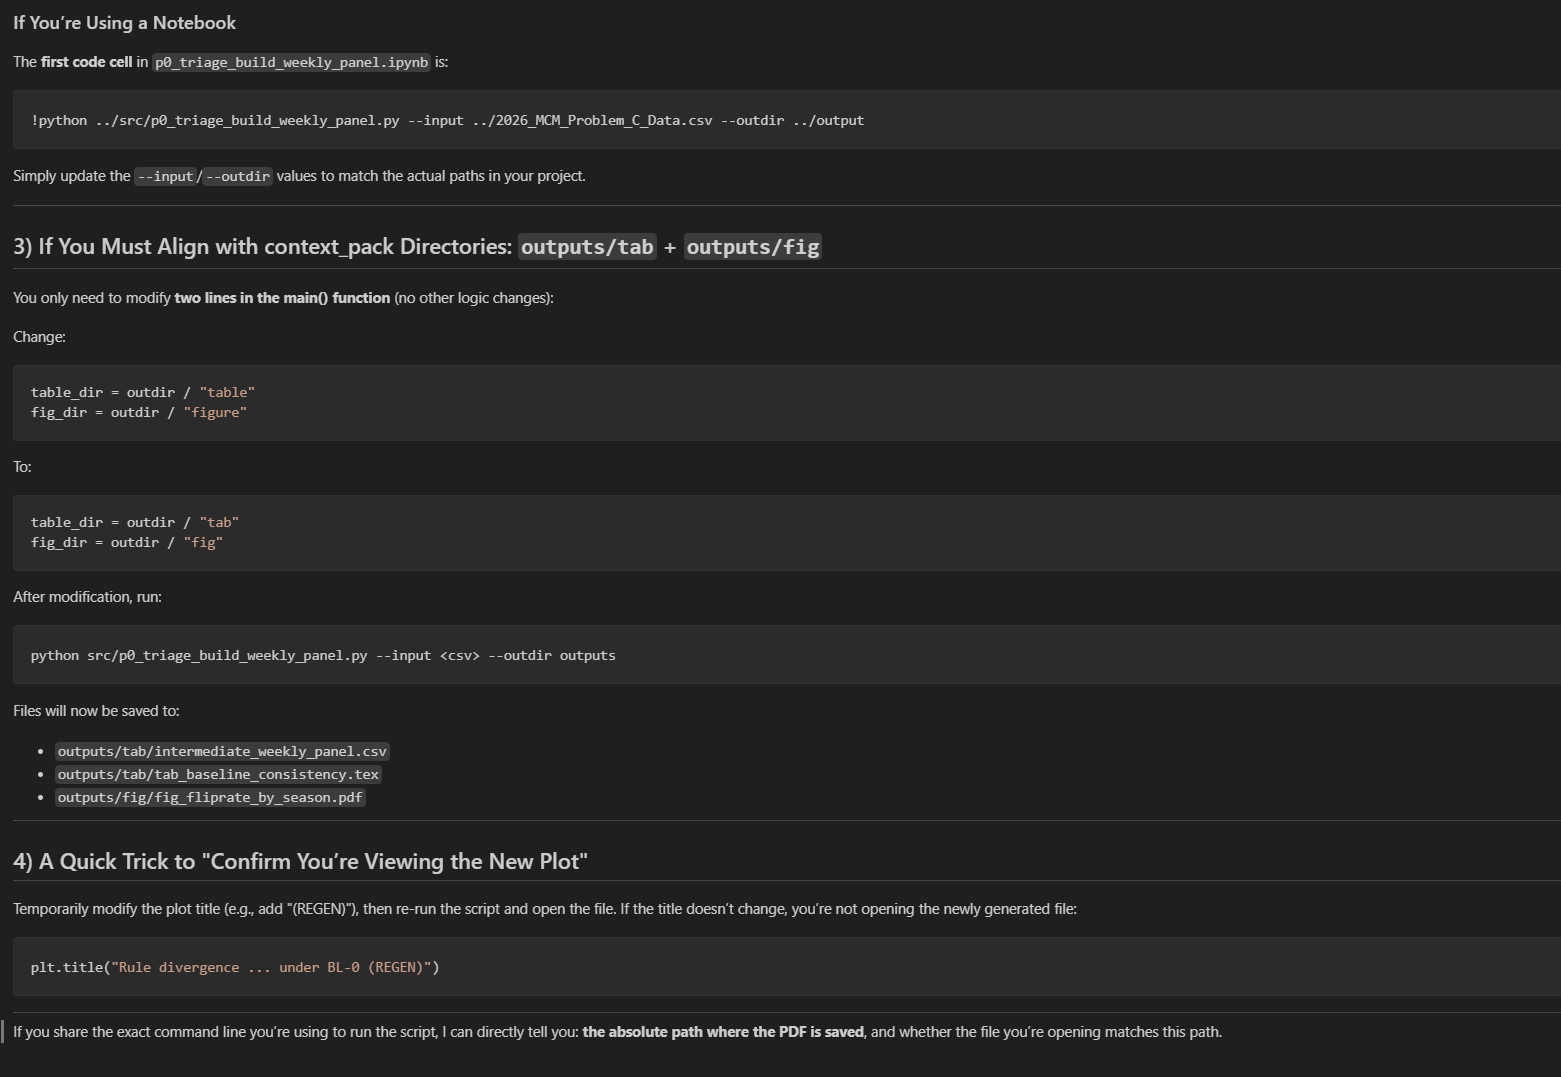
\includegraphics[width=0.9\linewidth]{report_on_use_of_ai/pho/4_2.png}
  \caption{ChatGPT Query 4 Output Screenshot}
  \label{fig:chatgpt_query_4_output_2}
\end{figure}


\textbf{\href{https://github.com/charles65536/model2026-2/blob/main/report_on_use_of_ai/chatgpt_5_input_and_output.md}{ChatGPT Query 5:}}\\
\textbf{Input:}
Currently, our .py code files are located at 2026\_MCM/src/LI\_play\_data/*.py, and we expect the generated charts to be saved to 2026\_MCM/output/fig (or 2026\_MCM/output/tab for tables, and the required data to be saved to 2026\_MCM/output/data\_cleaned).
I have several questions:\\
(a) Do we need to manually create the output/fig and output/tab directories in advance?\\
(b) If not, do we need to modify the paths in the Python files, and how? (We do not plan to use .ipynb files.)\\
(c) After modifying the paths in the files, how should I run the script on a Windows computer to generate the new files? Will the newly generated files overwrite the existing ones after running the script?\\
\textbf{Output:}
\begin{figure}[H]
  \centering
  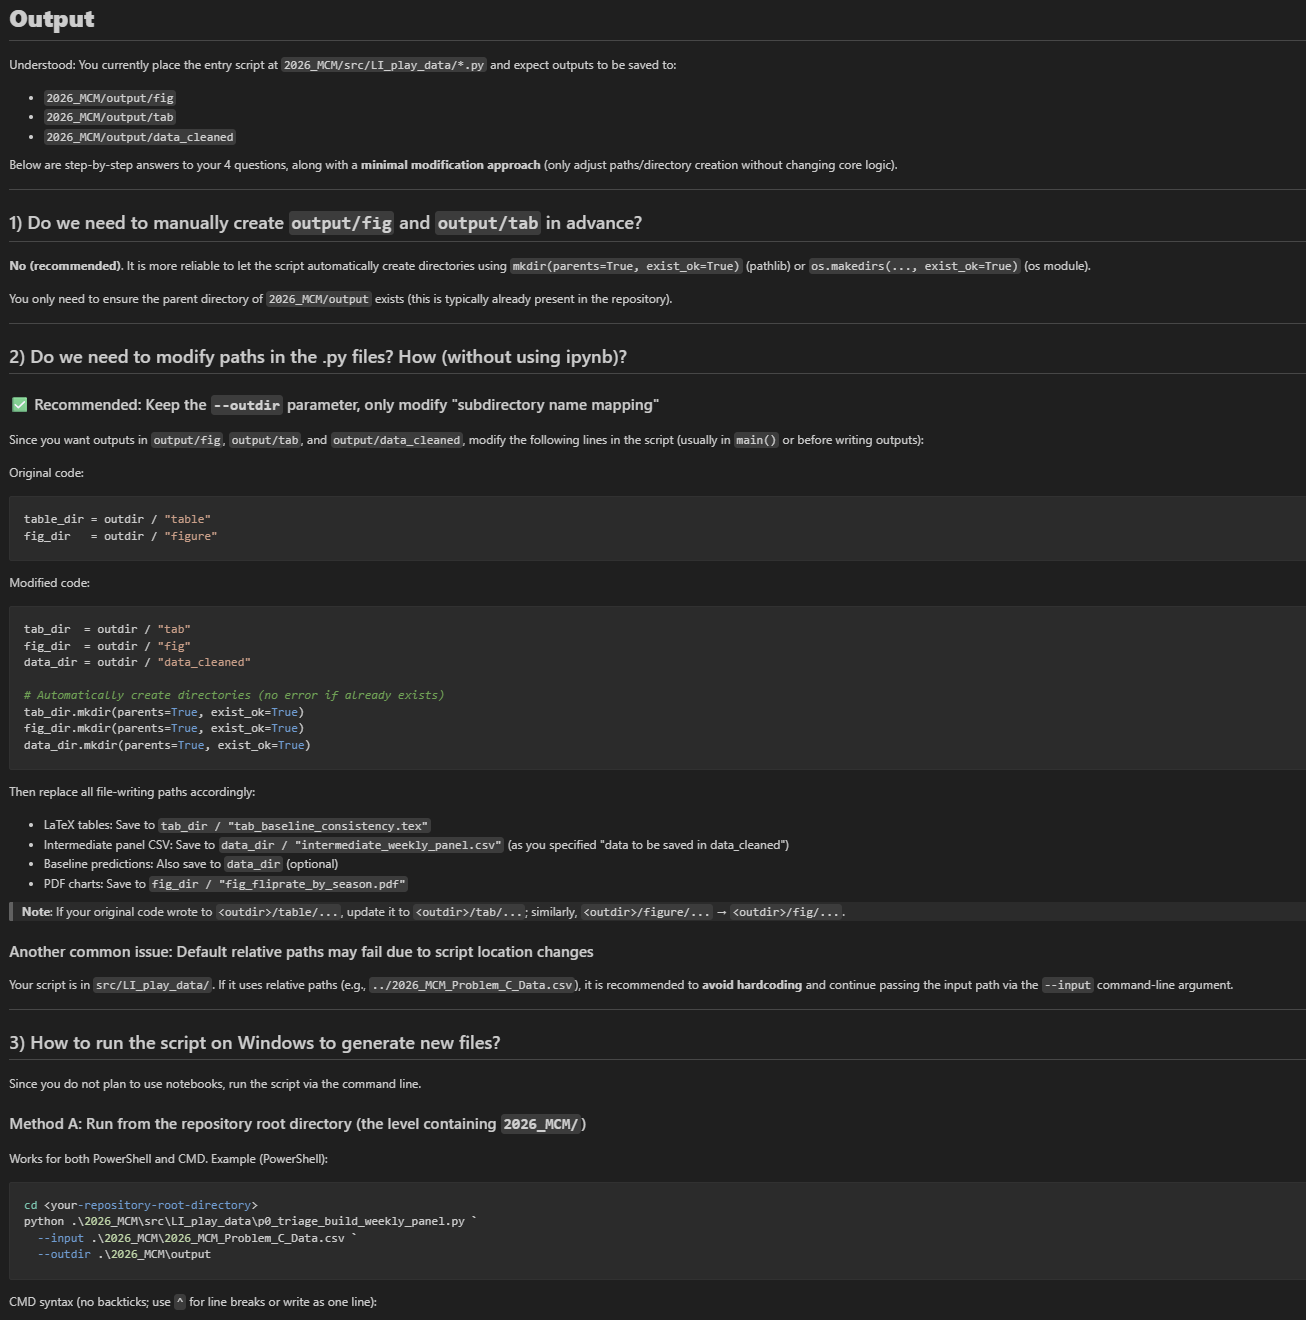
\includegraphics[width=0.9\linewidth]{report_on_use_of_ai/pho/5_1.png}
  \caption{ChatGPT Query 5 Output Screenshot}
  \label{fig:chatgpt_query_5_output}
\end{figure}
\begin{figure}[H]
  \centering
  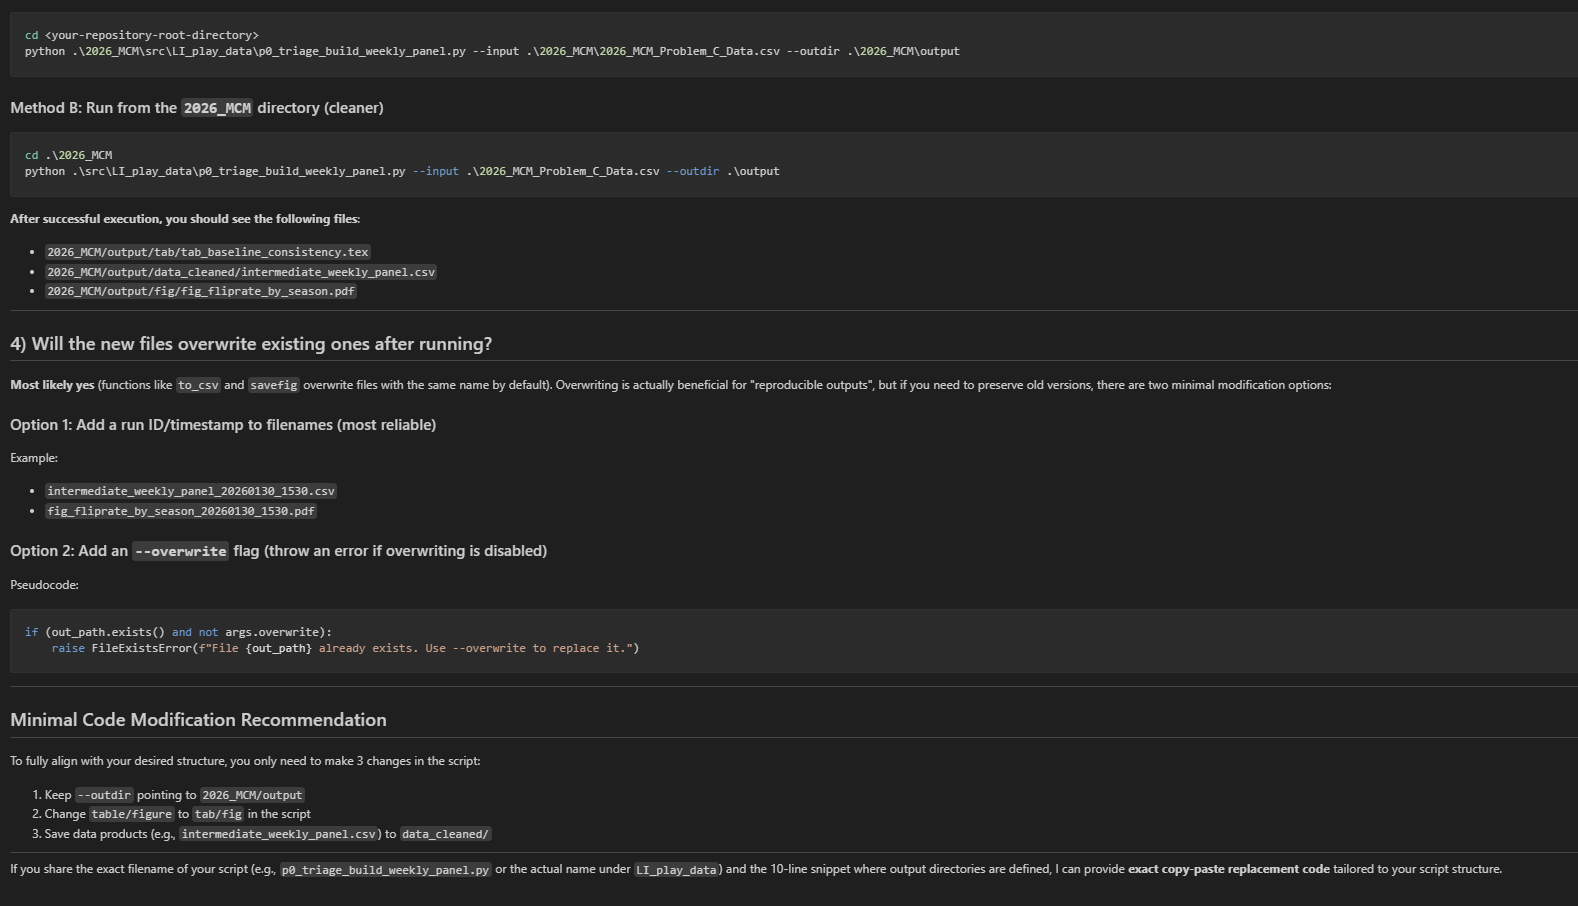
\includegraphics[width=0.9\linewidth]{report_on_use_of_ai/pho/5_2.png}
  \caption{ChatGPT Query 5 Output Screenshot}
  \label{fig:chatgpt_query_5_output_2}
\end{figure}



\textbf{\href{https://github.com/charles65536/model2026-2/blob/main/report_on_use_of_ai/chatgpt_6_input_and_output.md}{ChatGPT Query 6:}}\\
\begin{figure}[H]
  \centering
  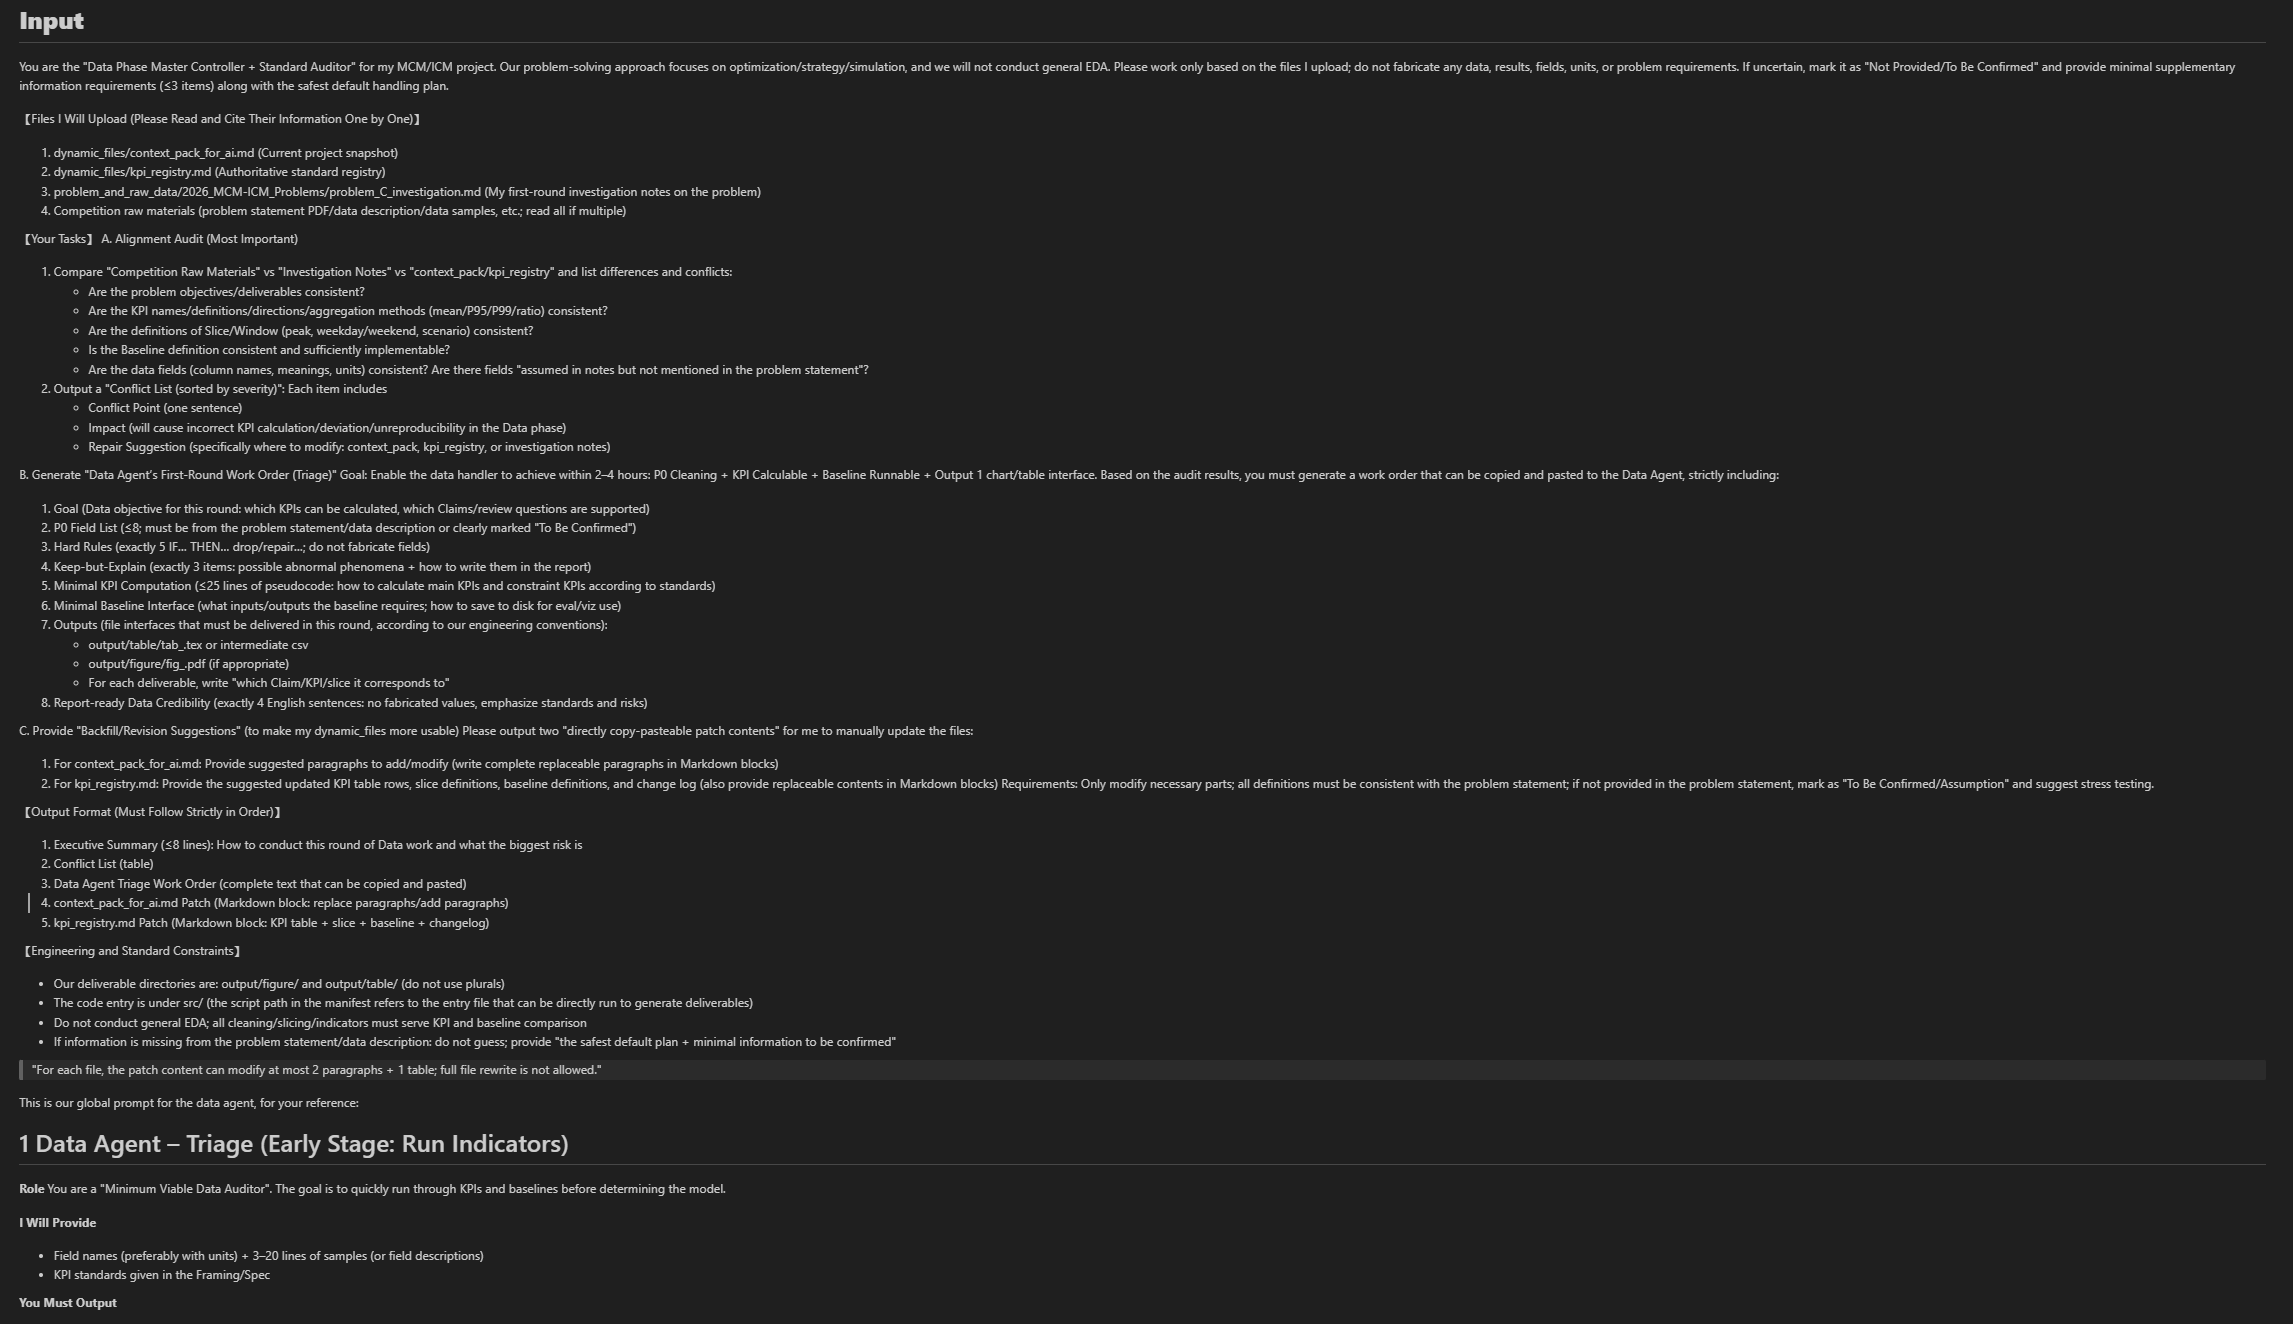
\includegraphics[width=0.9\linewidth]{report_on_use_of_ai/pho/6_1.png}
  \caption{ChatGPT Query 6 Output Screenshot}
  \label{fig:chatgpt_query_6_output}
\end{figure}
\begin{figure}[H]
  \centering
  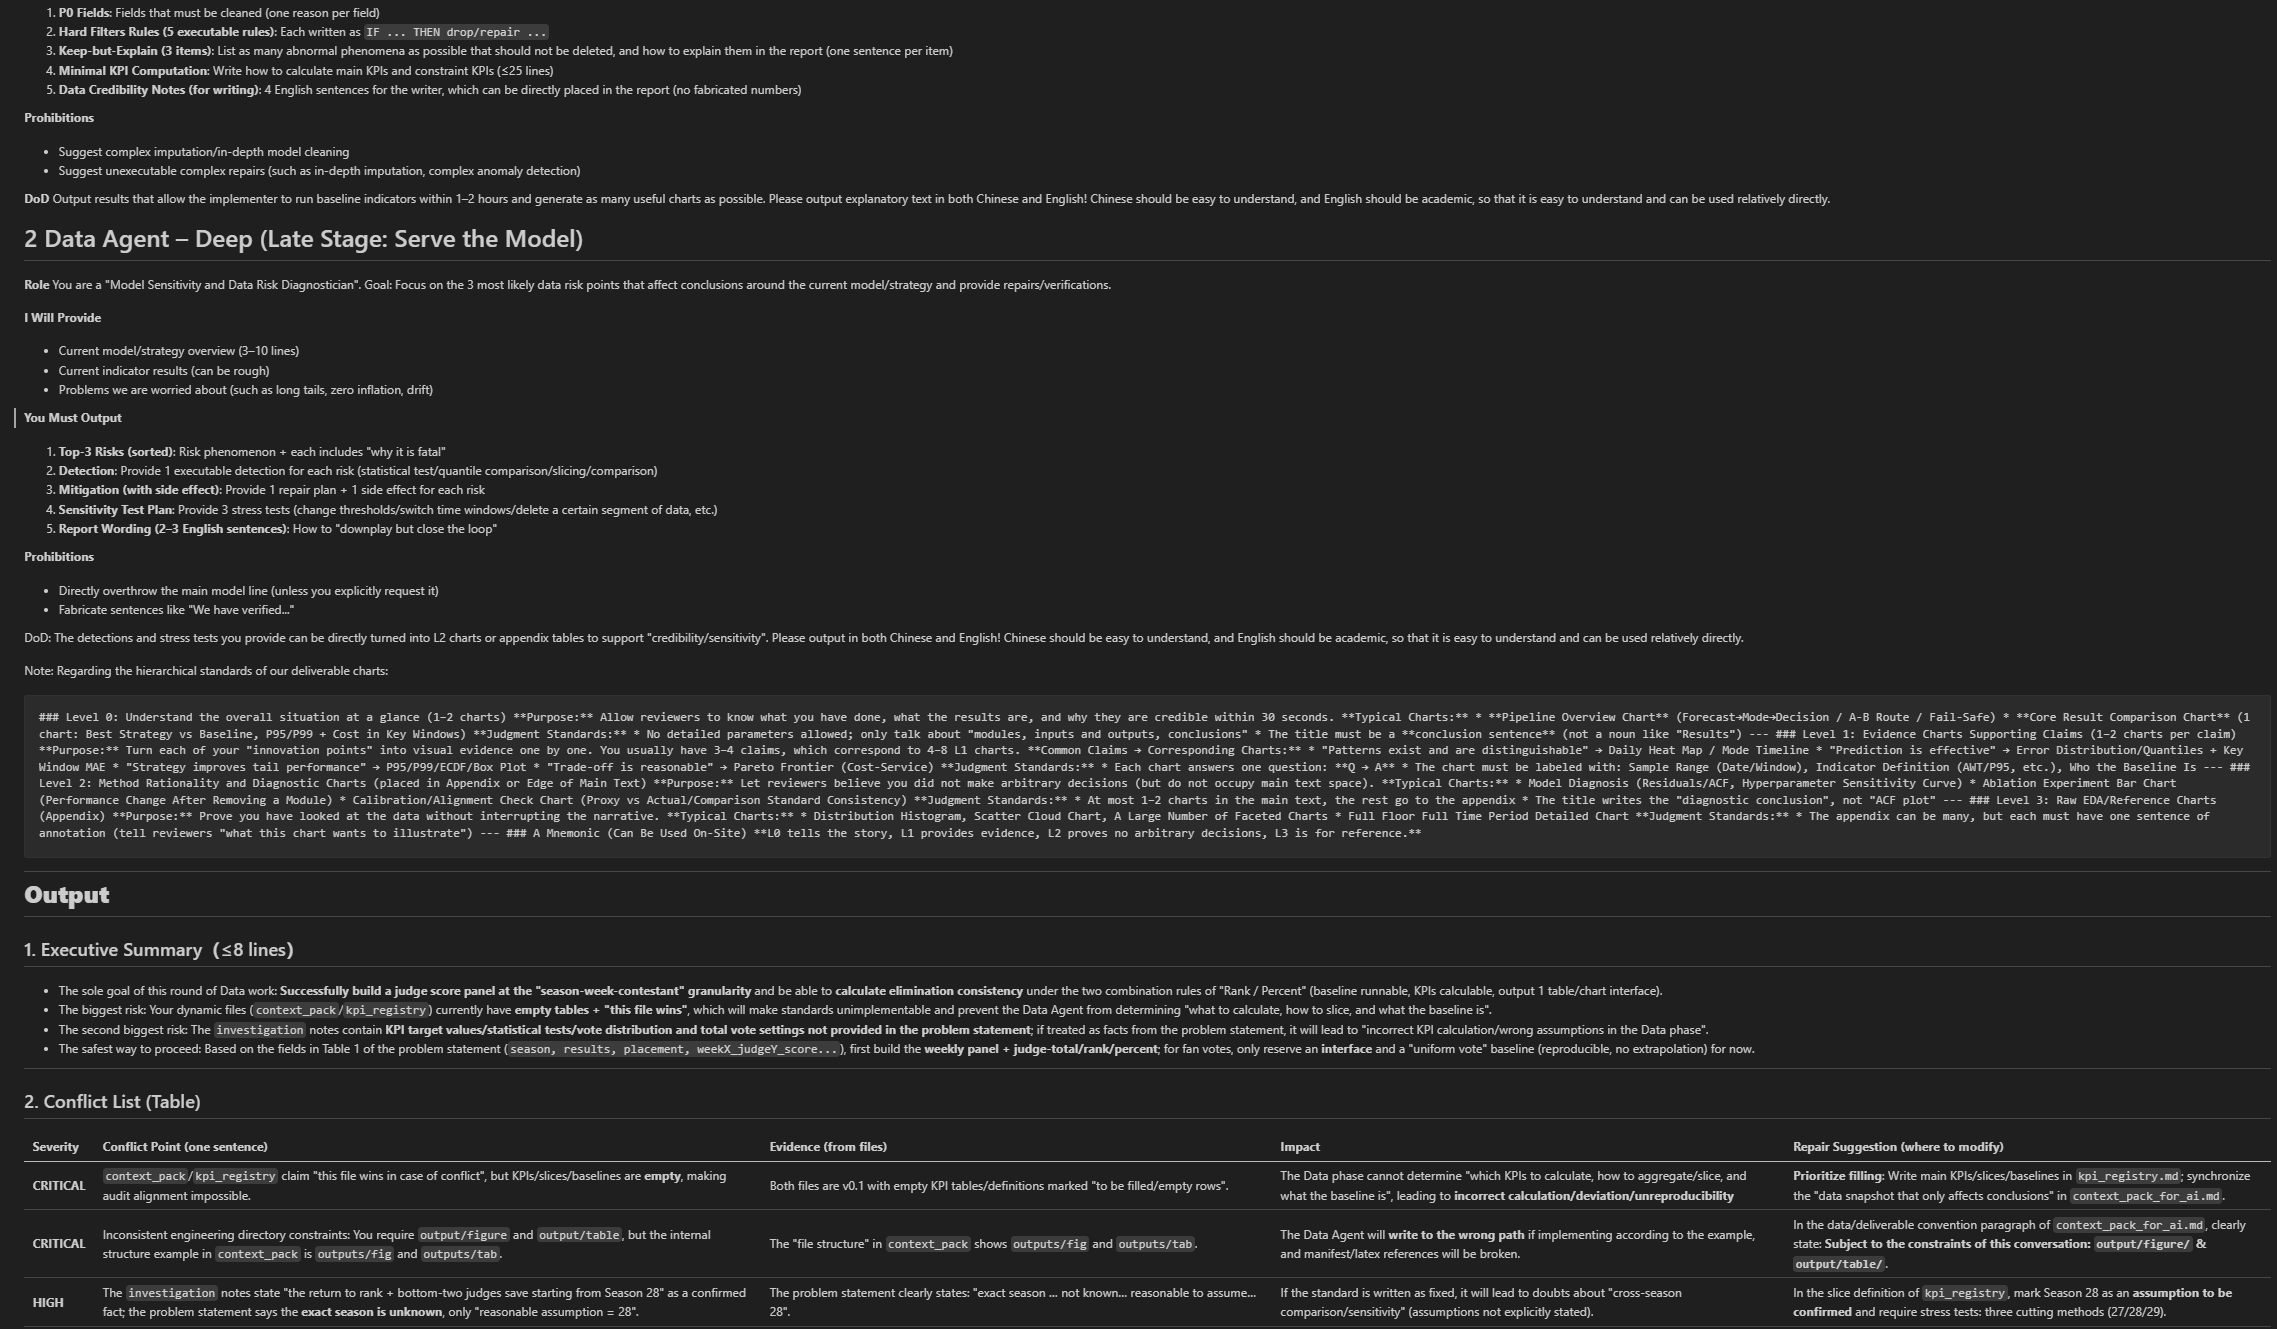
\includegraphics[width=0.9\linewidth]{report_on_use_of_ai/pho/6_2.png}
  \caption{ChatGPT Query 6 Output Screenshot}
  \label{fig:chatgpt_query_6_output2}
\end{figure}
\begin{figure}[H]
  \centering
  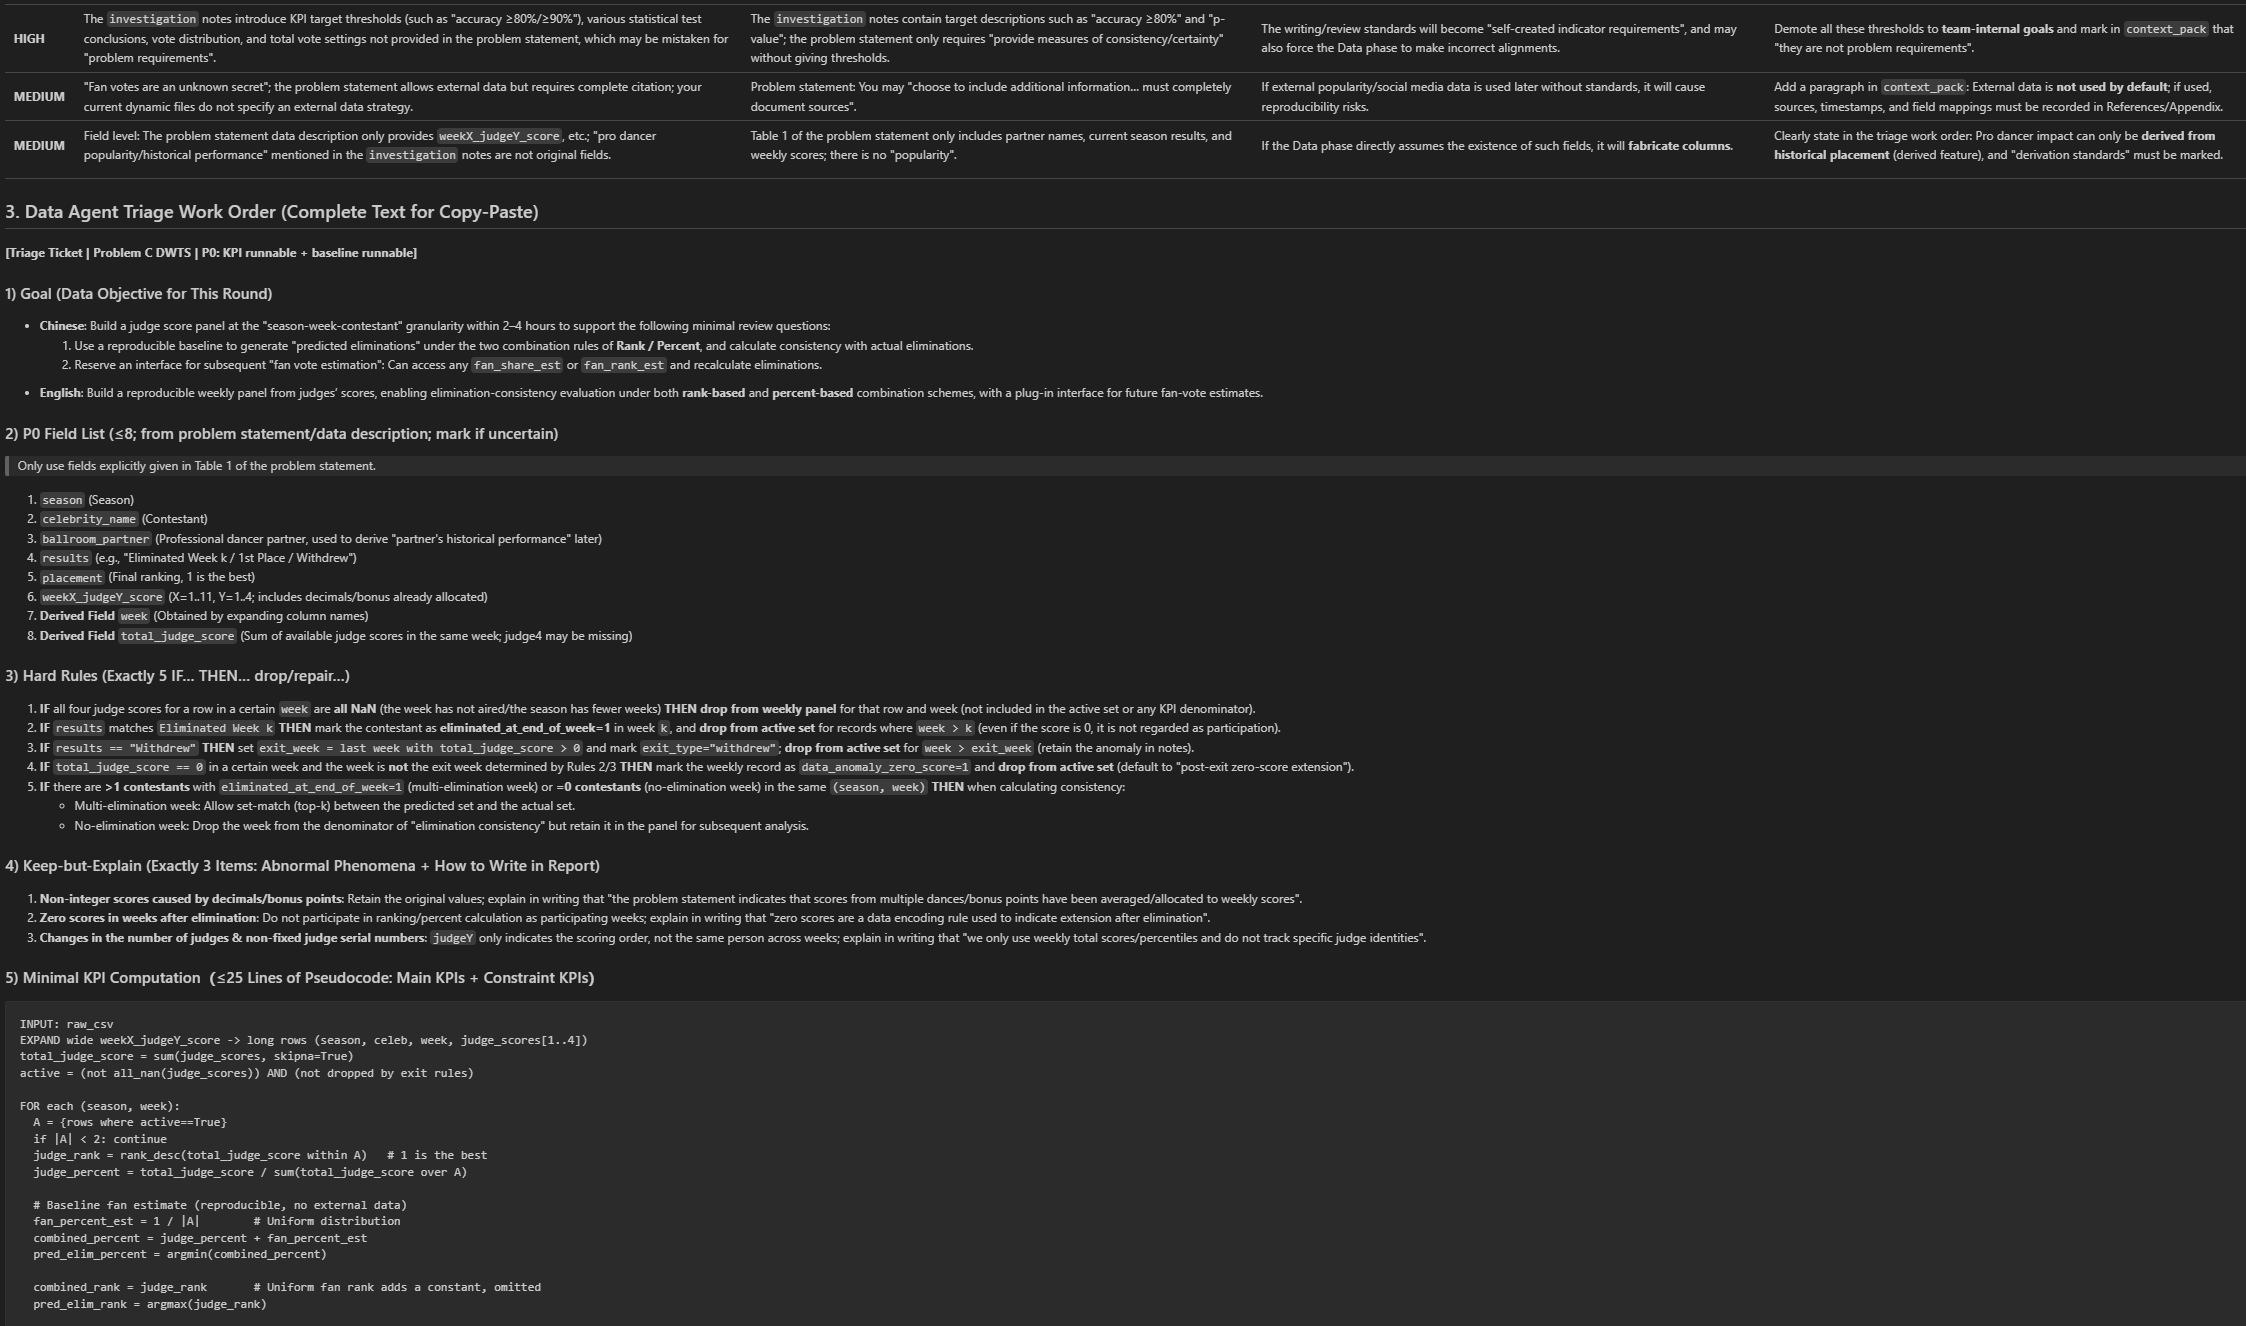
\includegraphics[width=0.9\linewidth]{report_on_use_of_ai/pho/6_3.png}
  \caption{ChatGPT Query 6 Output Screenshot}
  \label{fig:chatgpt_query_6_output3}
\end{figure}
\begin{figure}[H]
  \centering
  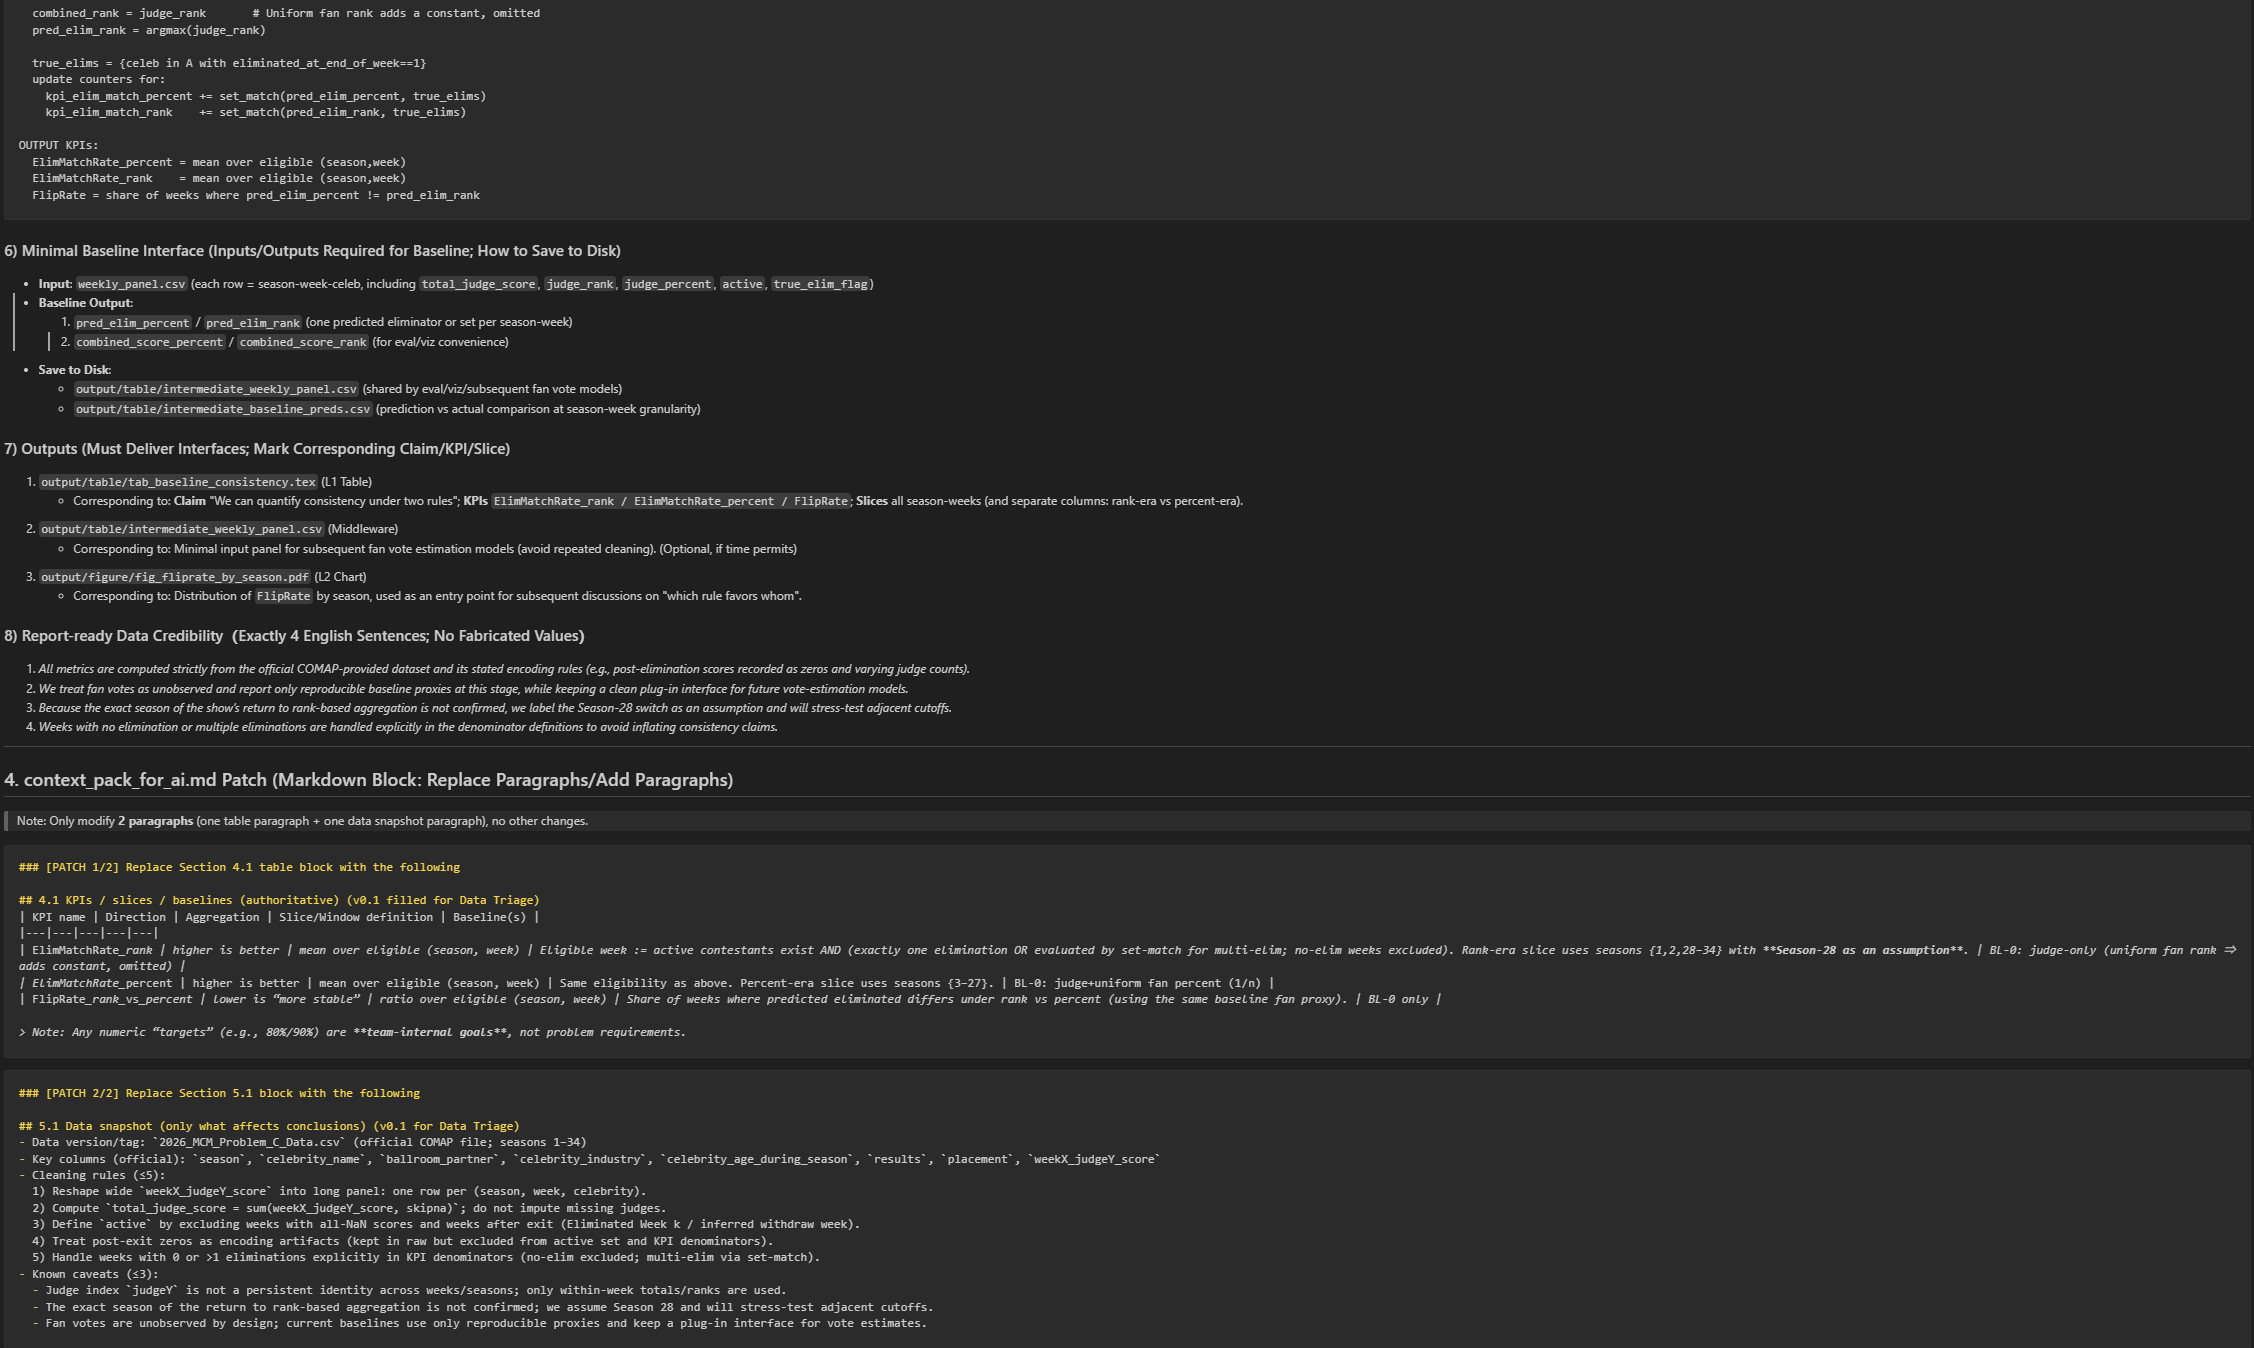
\includegraphics[width=0.9\linewidth]{report_on_use_of_ai/pho/6_4.png}
  \caption{ChatGPT Query 6 Output Screenshot}
  \label{fig:chatgpt_query_6_output4}
\end{figure}
\begin{figure}[H]
  \centering
  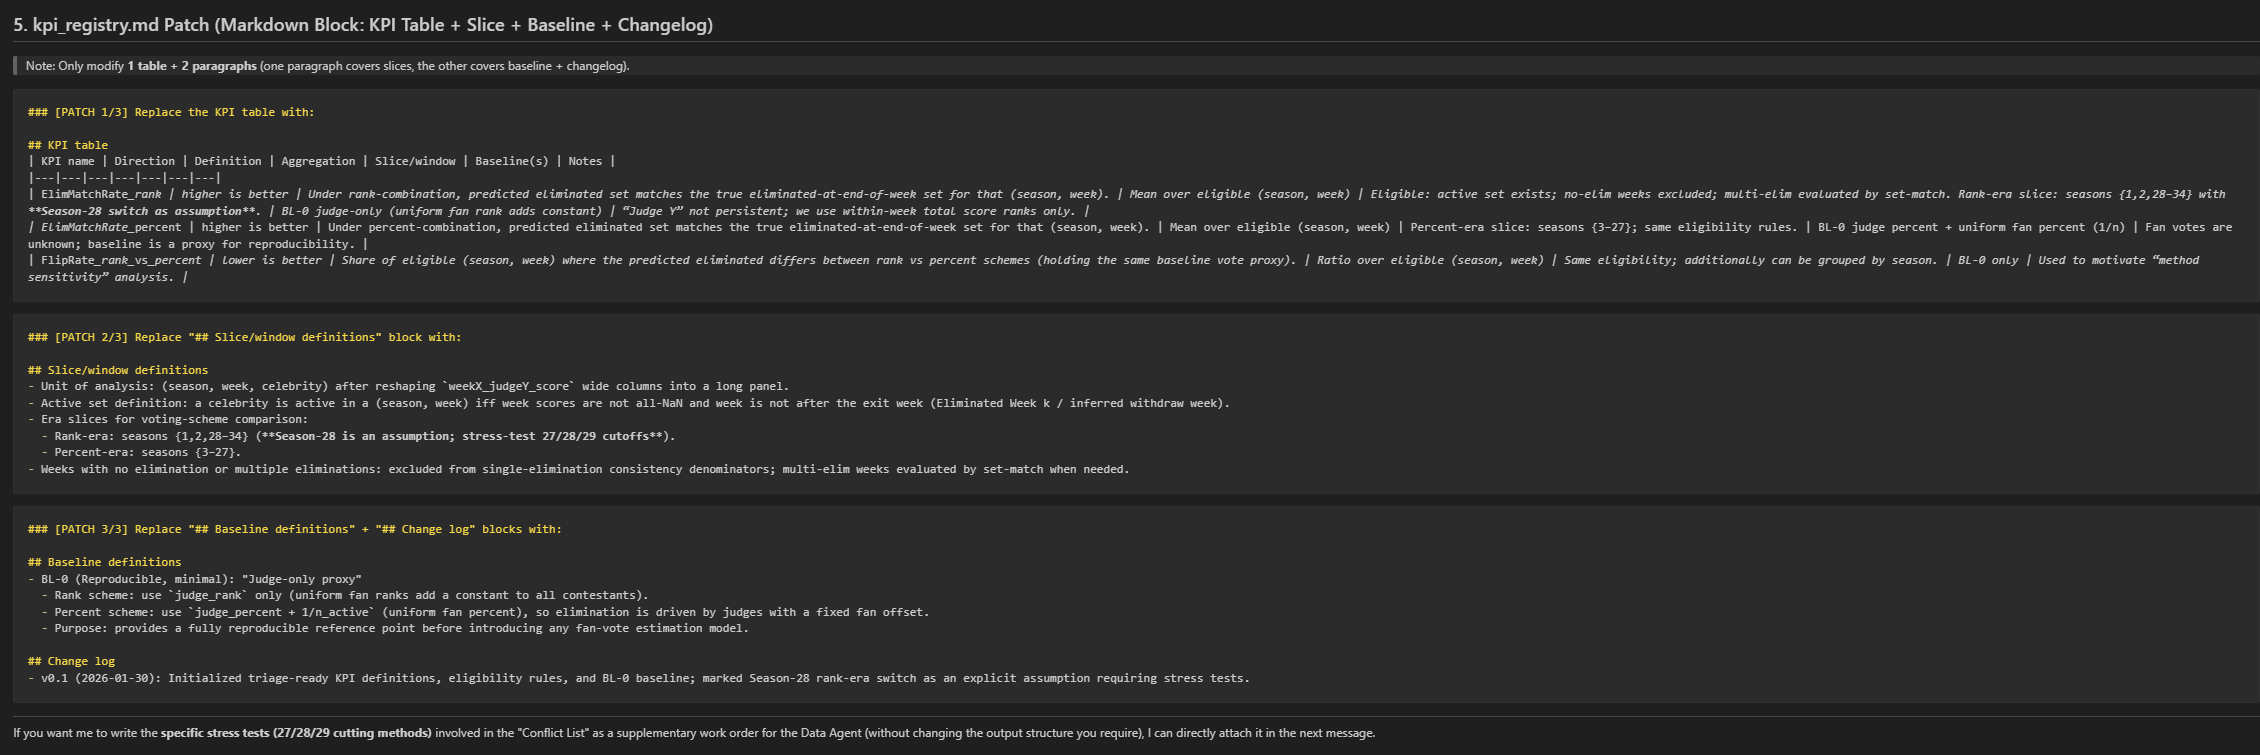
\includegraphics[width=0.9\linewidth]{report_on_use_of_ai/pho/6_5.png}
  \caption{ChatGPT Query 6 Output Screenshot}
  \label{fig:chatgpt_query_6_output5}
\end{figure}


\textbf{\href{https://github.com/charles65536/model2026-2/blob/main/report_on_use_of_ai/chatgpt_7_input_and_output.md}{ChatGPT Query 7:}}\\
\textbf{Input:}
What should we do regarding the previous conversation? Because the investigation file is non-authoritative; the files we feed to the agent do not include the investigation—it is only used for us to check if our framing/spec agent has any important omissions. Now clearly tell me how to use the information you provided above (e.g., 3. Place the Data Agent Triage work order in... file / place it separately in the conversation as a prompt).\\
\textbf{Output:}
\begin{figure}[H]
  \centering
  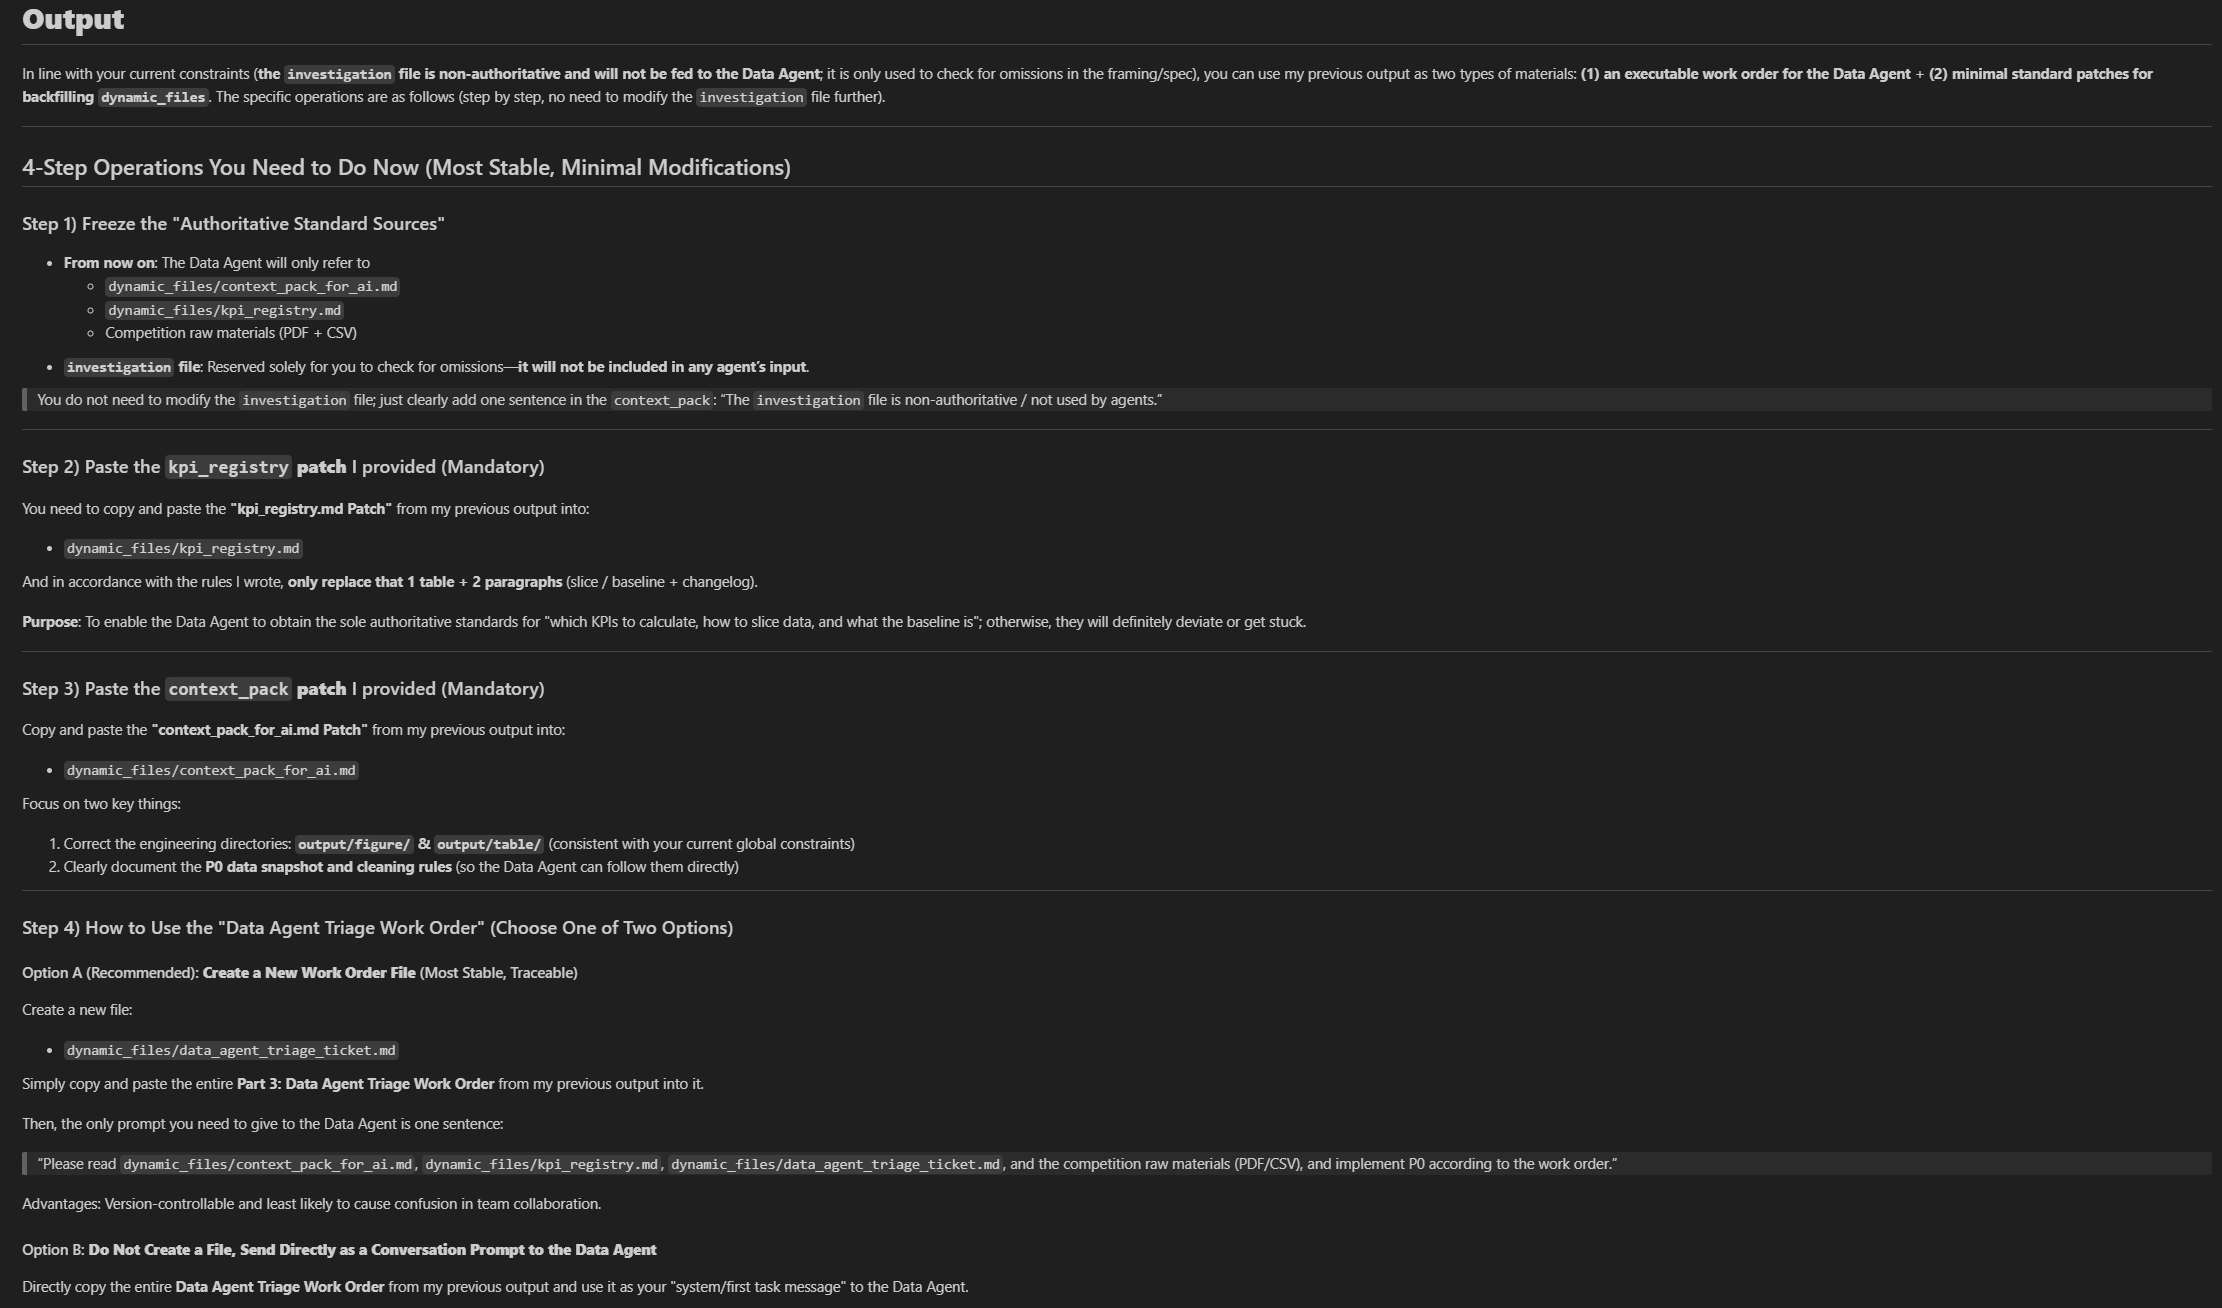
\includegraphics[width=0.9\linewidth]{report_on_use_of_ai/pho/7_1.png}
  \caption{ChatGPT Query 7 Output Screenshot}
  \label{fig:chatgpt_query_7_output}
\end{figure}
\begin{figure}[H]
  \centering
  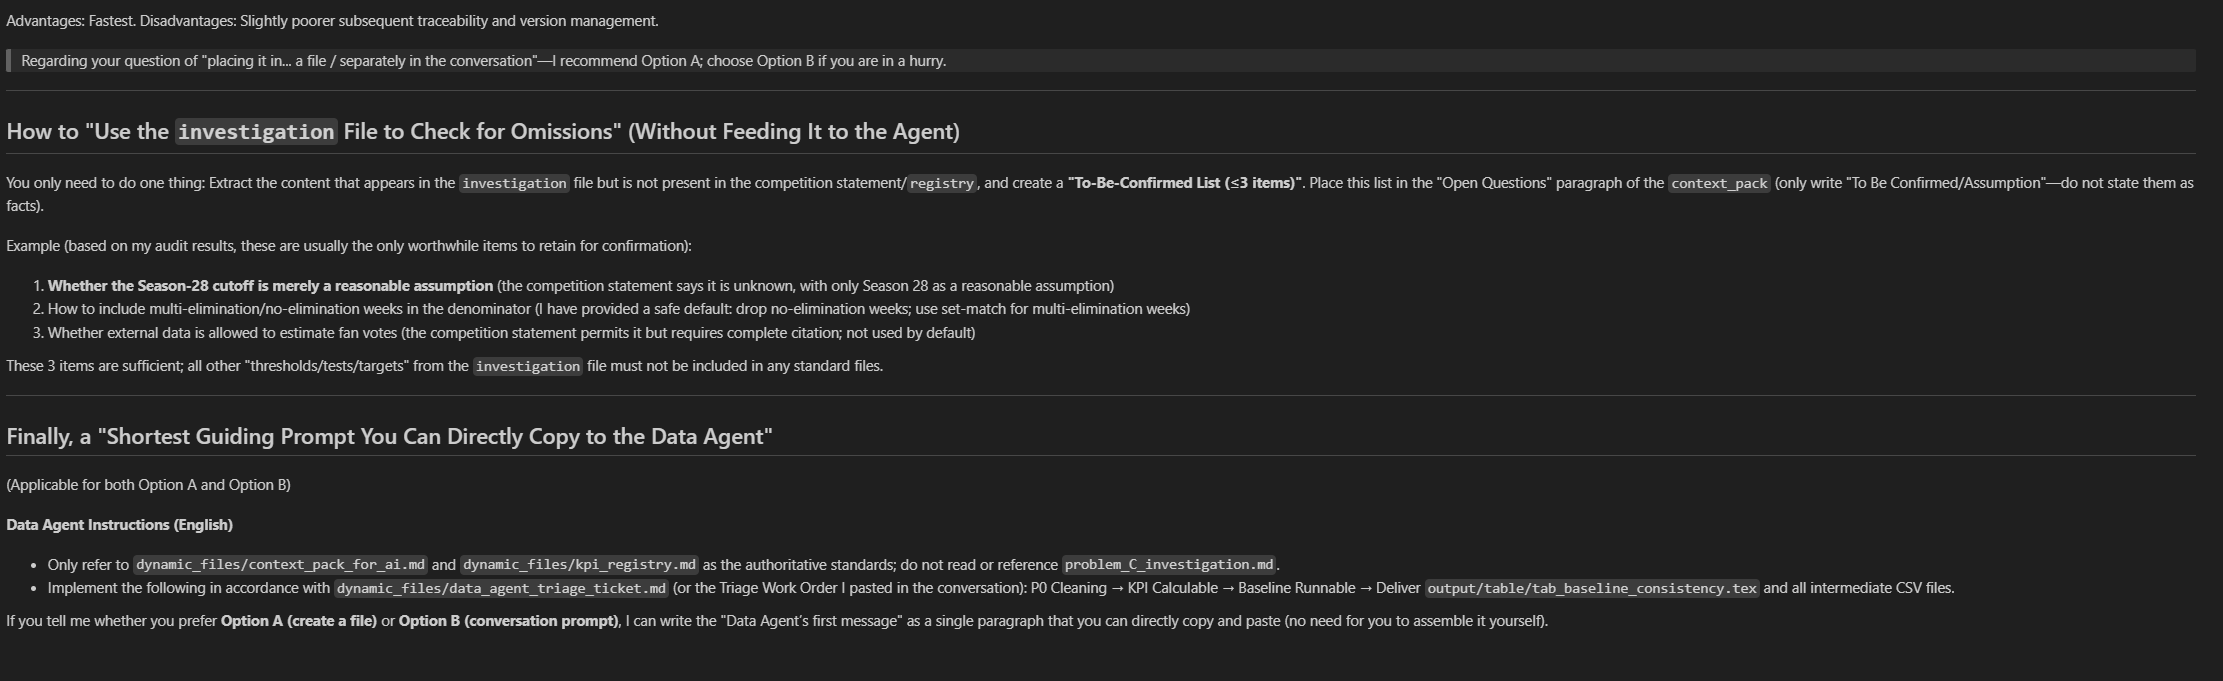
\includegraphics[width=0.9\linewidth]{report_on_use_of_ai/pho/7_2.png}
  \caption{ChatGPT Query 7 Output Screenshot}
  \label{fig:chatgpt_query_7_output2}
\end{figure}

\textbf{\href{https://github.com/charles65536/model2026-2/blob/main/report_on_use_of_ai/chatgpt_8_input_and_output.md}{ChatGPT Query 8:}}\\
\textbf{Input:}
'Handling of "Withdrew": Should it be "exclude after inferring the exit week" or "exclude the entire season from the consistency denominator"?
Consistency denominator: Exclude no-elimination weeks, use set-match for multi-elimination weeks (is this acceptable?).'
What is the best way to handle this? Is it part of our cleaning standards? If we only add this one-sentence patch, will it cause huge problems in subsequent data processing?\\
\textbf{Output:}
\begin{figure}[H]
  \centering
  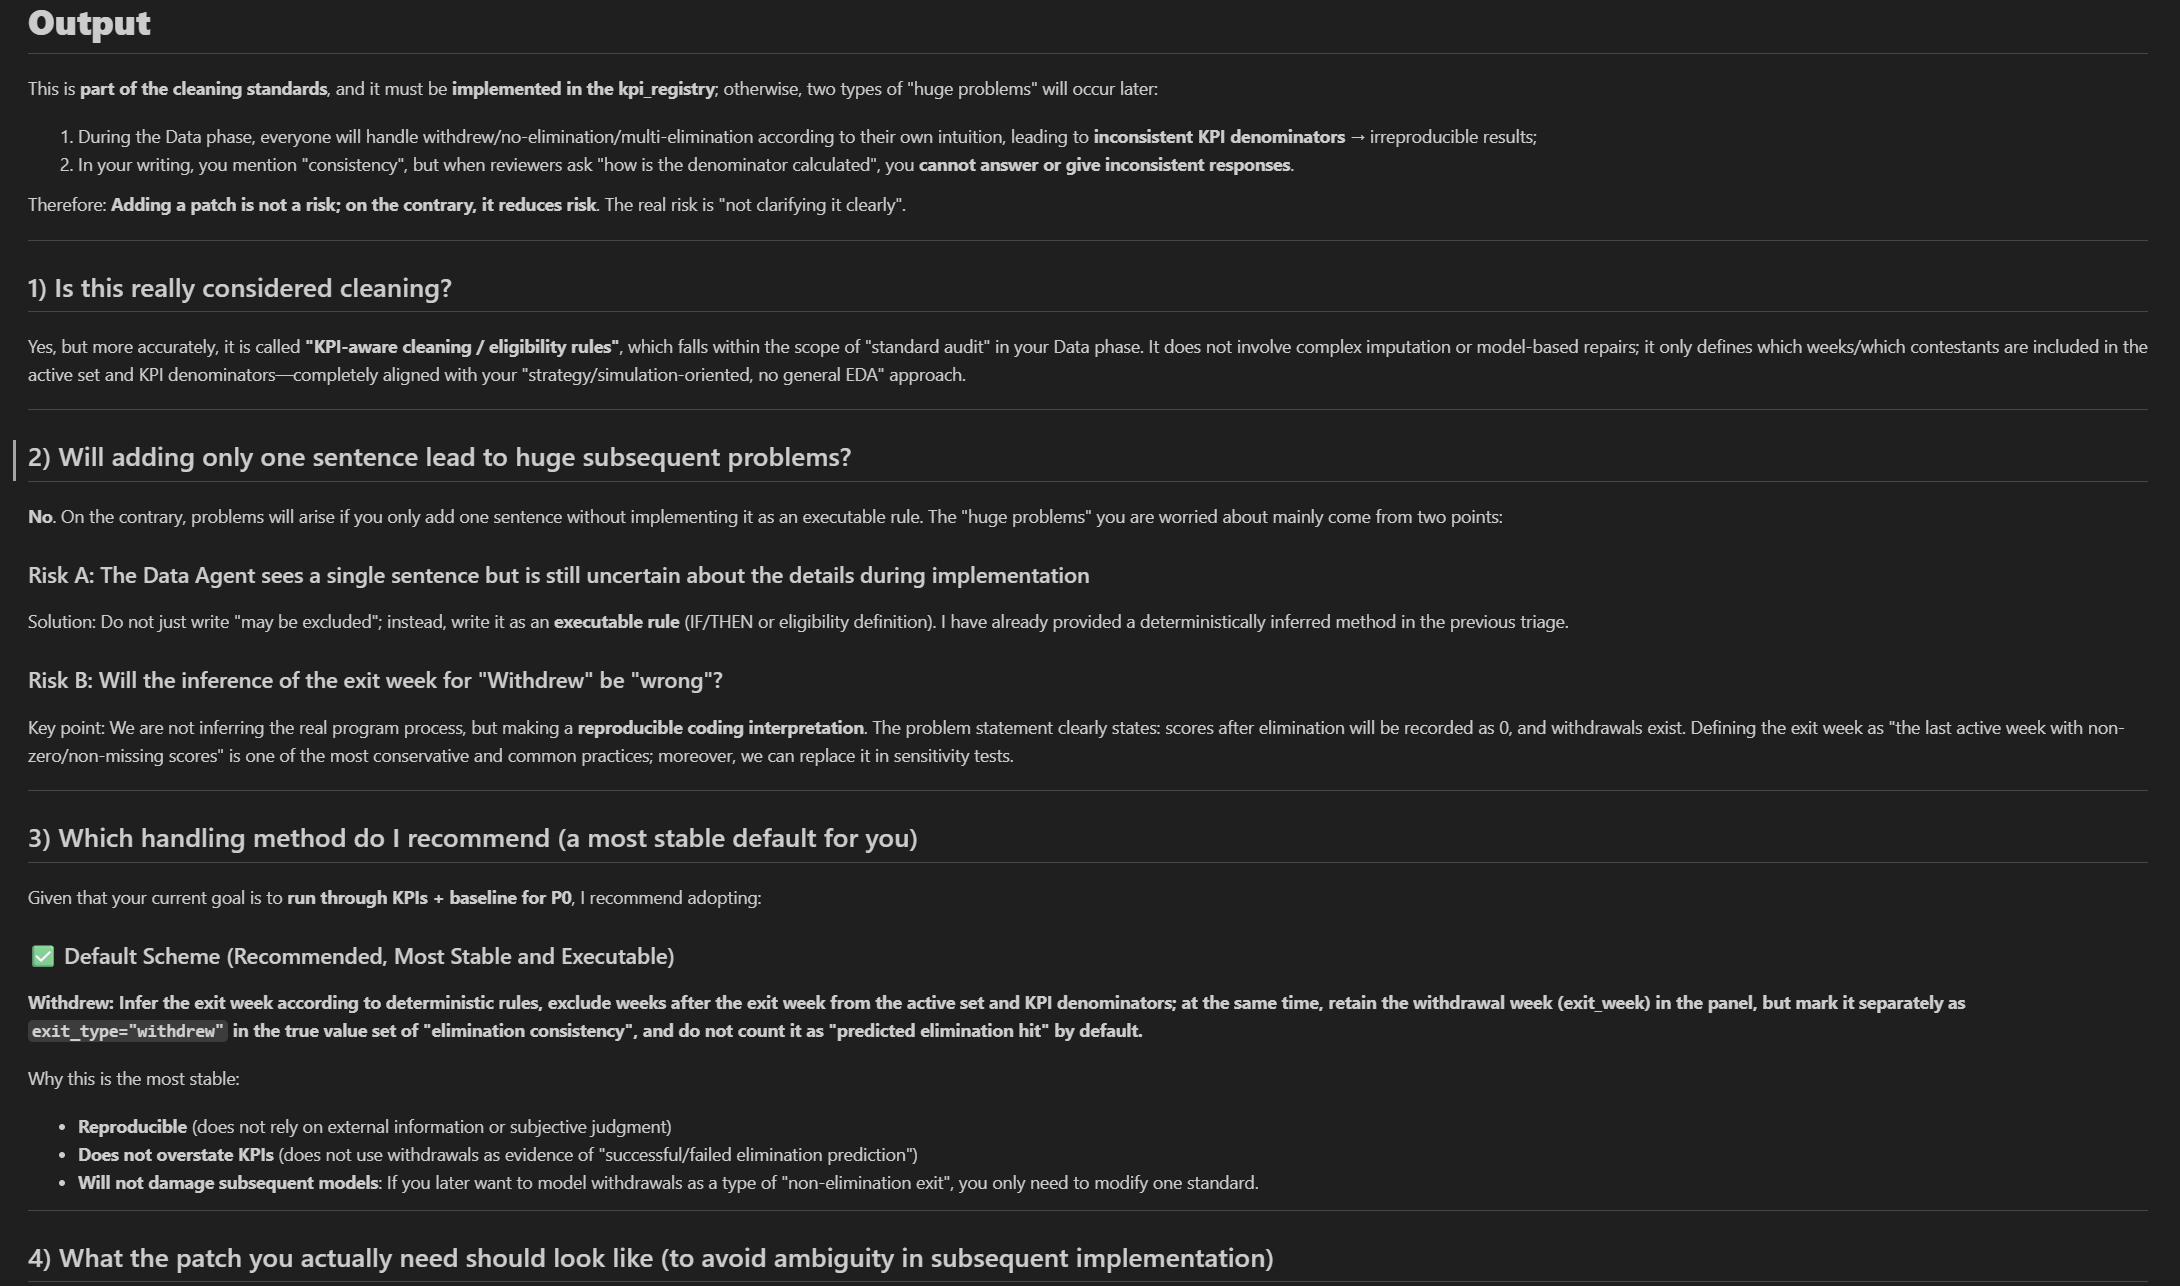
\includegraphics[width=0.9\linewidth]{report_on_use_of_ai/pho/81.png}
  \caption{ChatGPT Query 8 Output Screenshot}
  \label{fig:chatgpt_query_8_output}
\end{figure}
\begin{figure}[H]
  \centering
  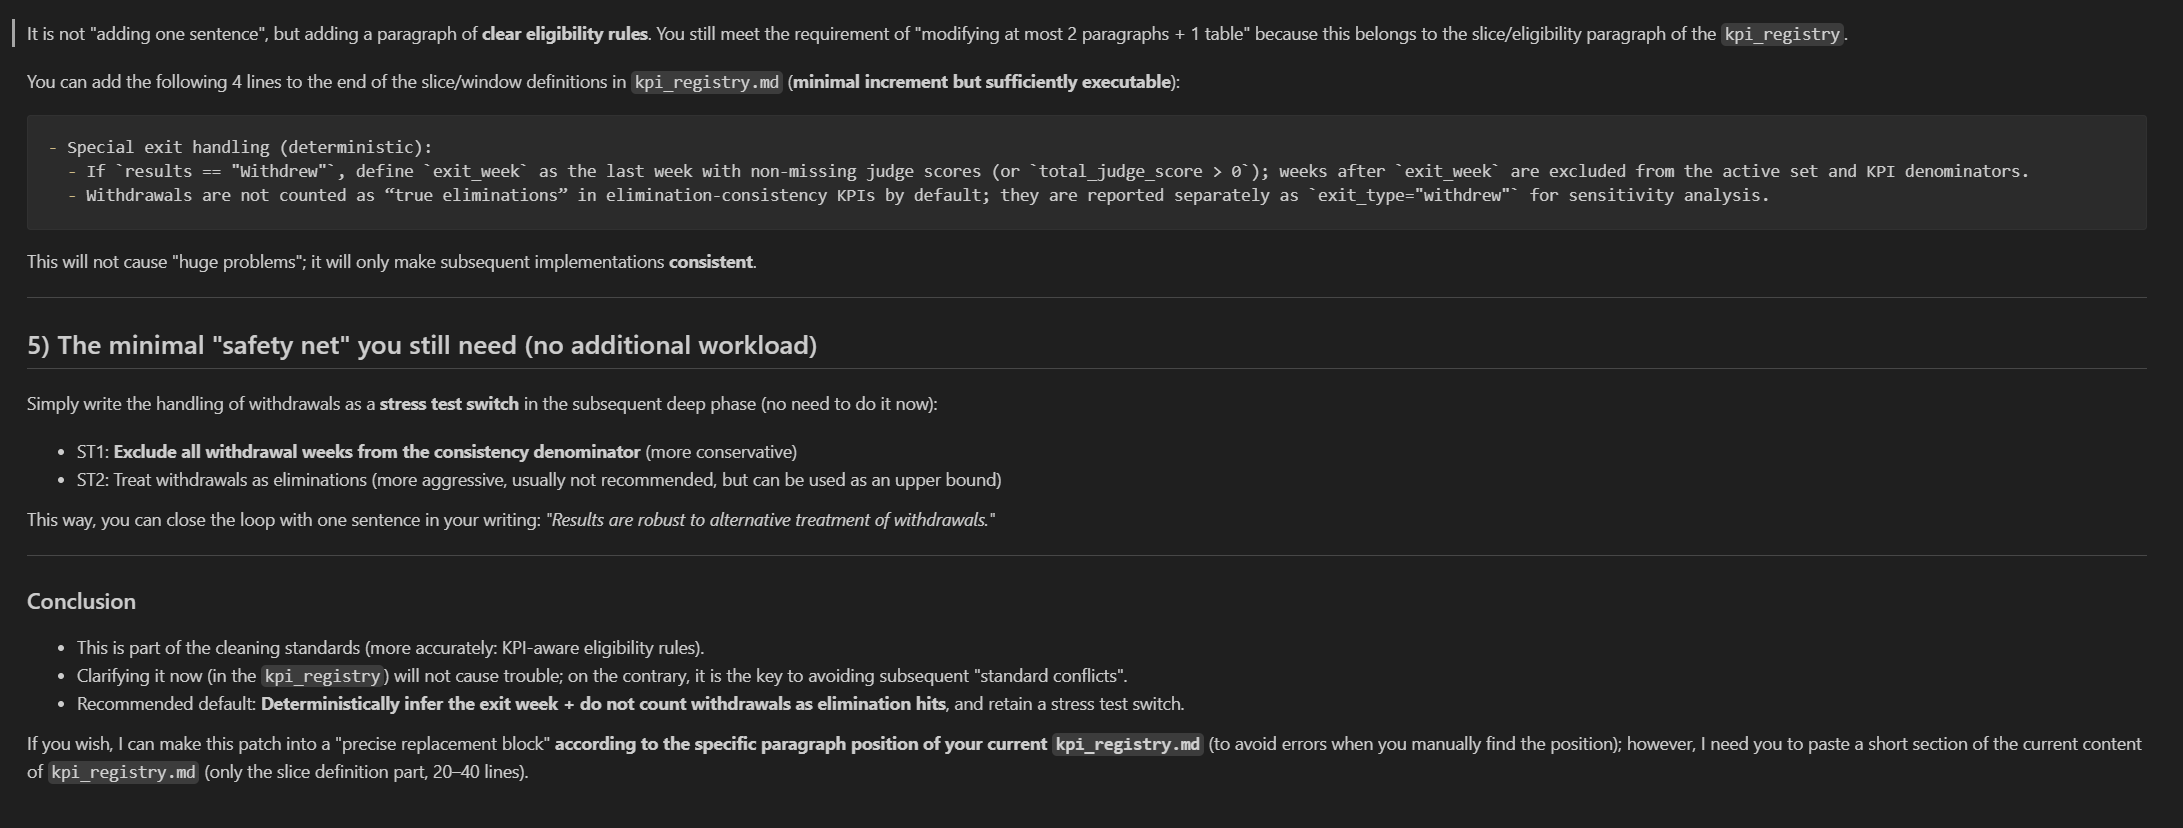
\includegraphics[width=0.9\linewidth]{report_on_use_of_ai/pho/82.png}
  \caption{ChatGPT Query 8 Output Screenshot}
  \label{fig:chatgpt_query_8_output2}
\end{figure}


\textbf{\href{https://github.com/charles65536/model2026-2/blob/main/report_on_use_of_ai/chatgpt_9_input_and_output.md}{ChatGPT Query 9:}}\\
\\
\textbf{Input:}
\begin{figure}[H]
  \centering
  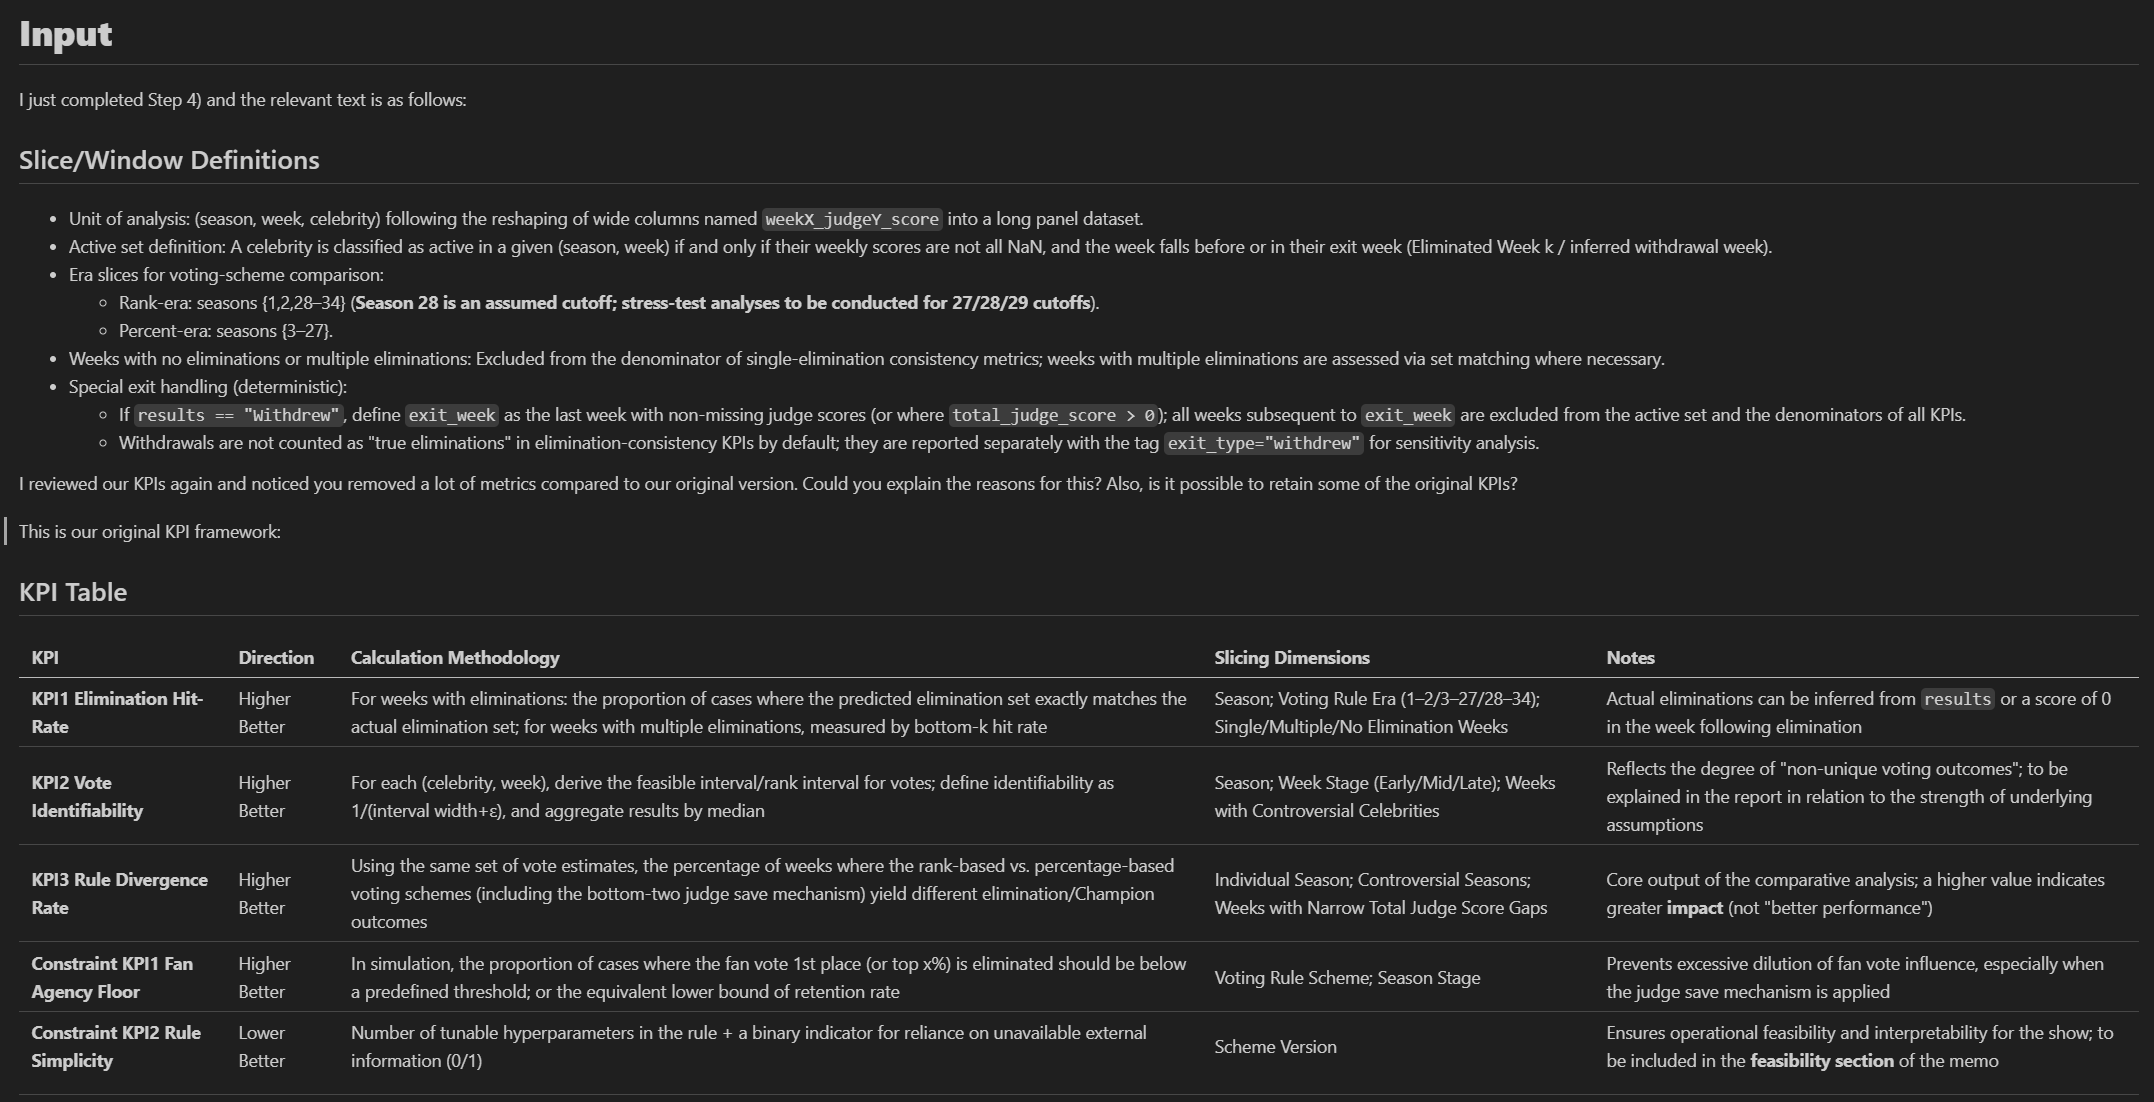
\includegraphics[width=0.9\linewidth]{report_on_use_of_ai/pho/91.png}
  \caption{ChatGPT Query 9 Input Screenshot}
  \label{fig:chatgpt_query_9_input}
\end{figure}

\textbf{Output:}
\begin{figure}[H]
  \centering
  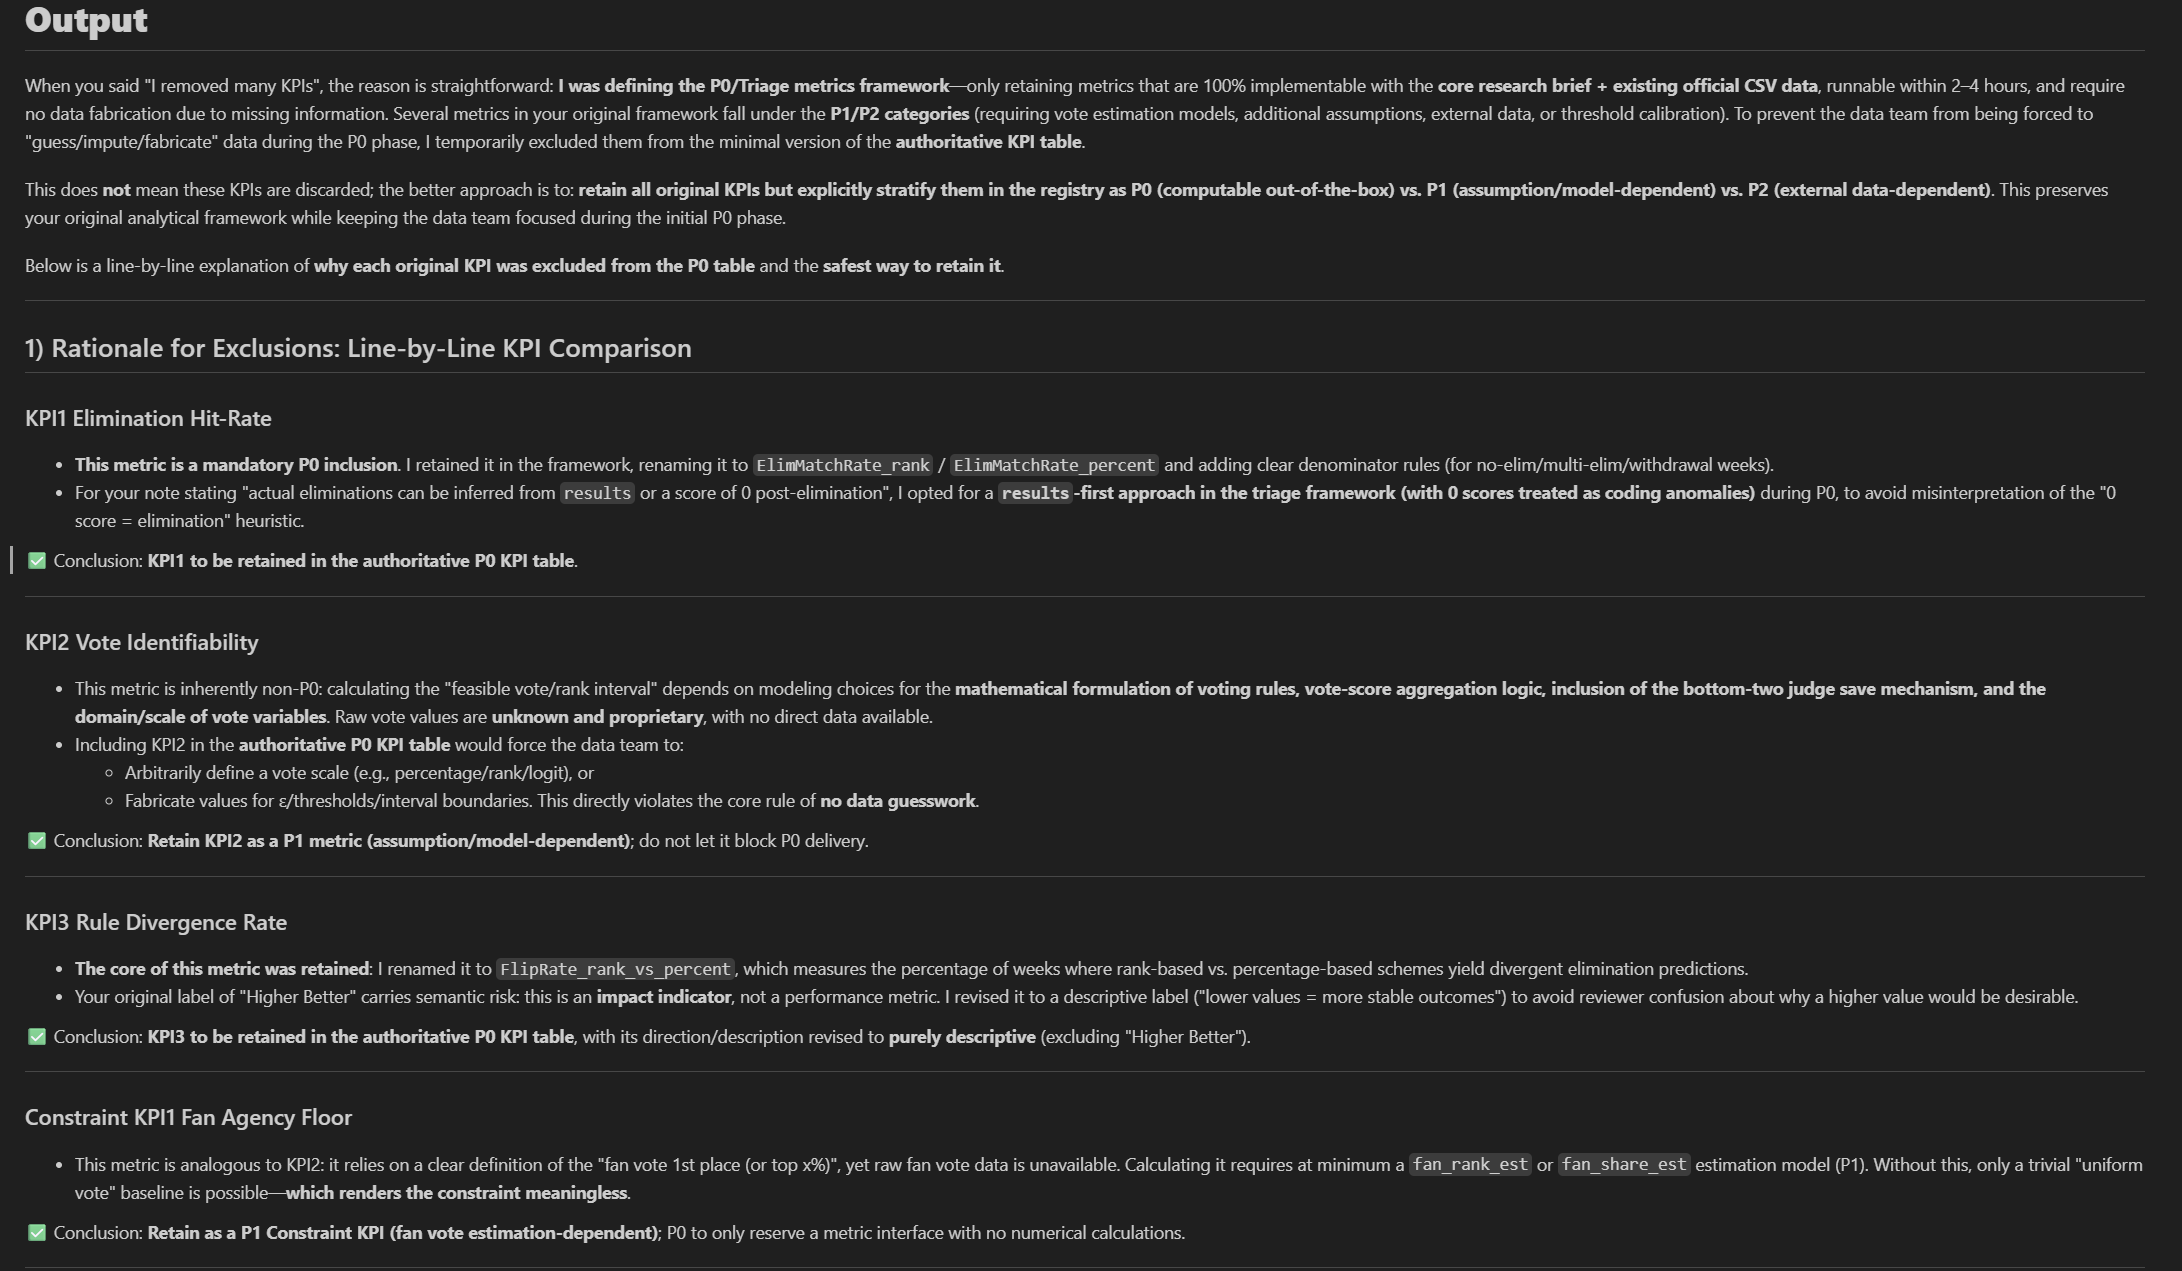
\includegraphics[width=0.9\linewidth]{report_on_use_of_ai/pho/92.png}
  \caption{ChatGPT Query 9 Output Screenshot}
  \label{fig:chatgpt_query_9_output}
\end{figure}
\begin{figure}[H]
  \centering
  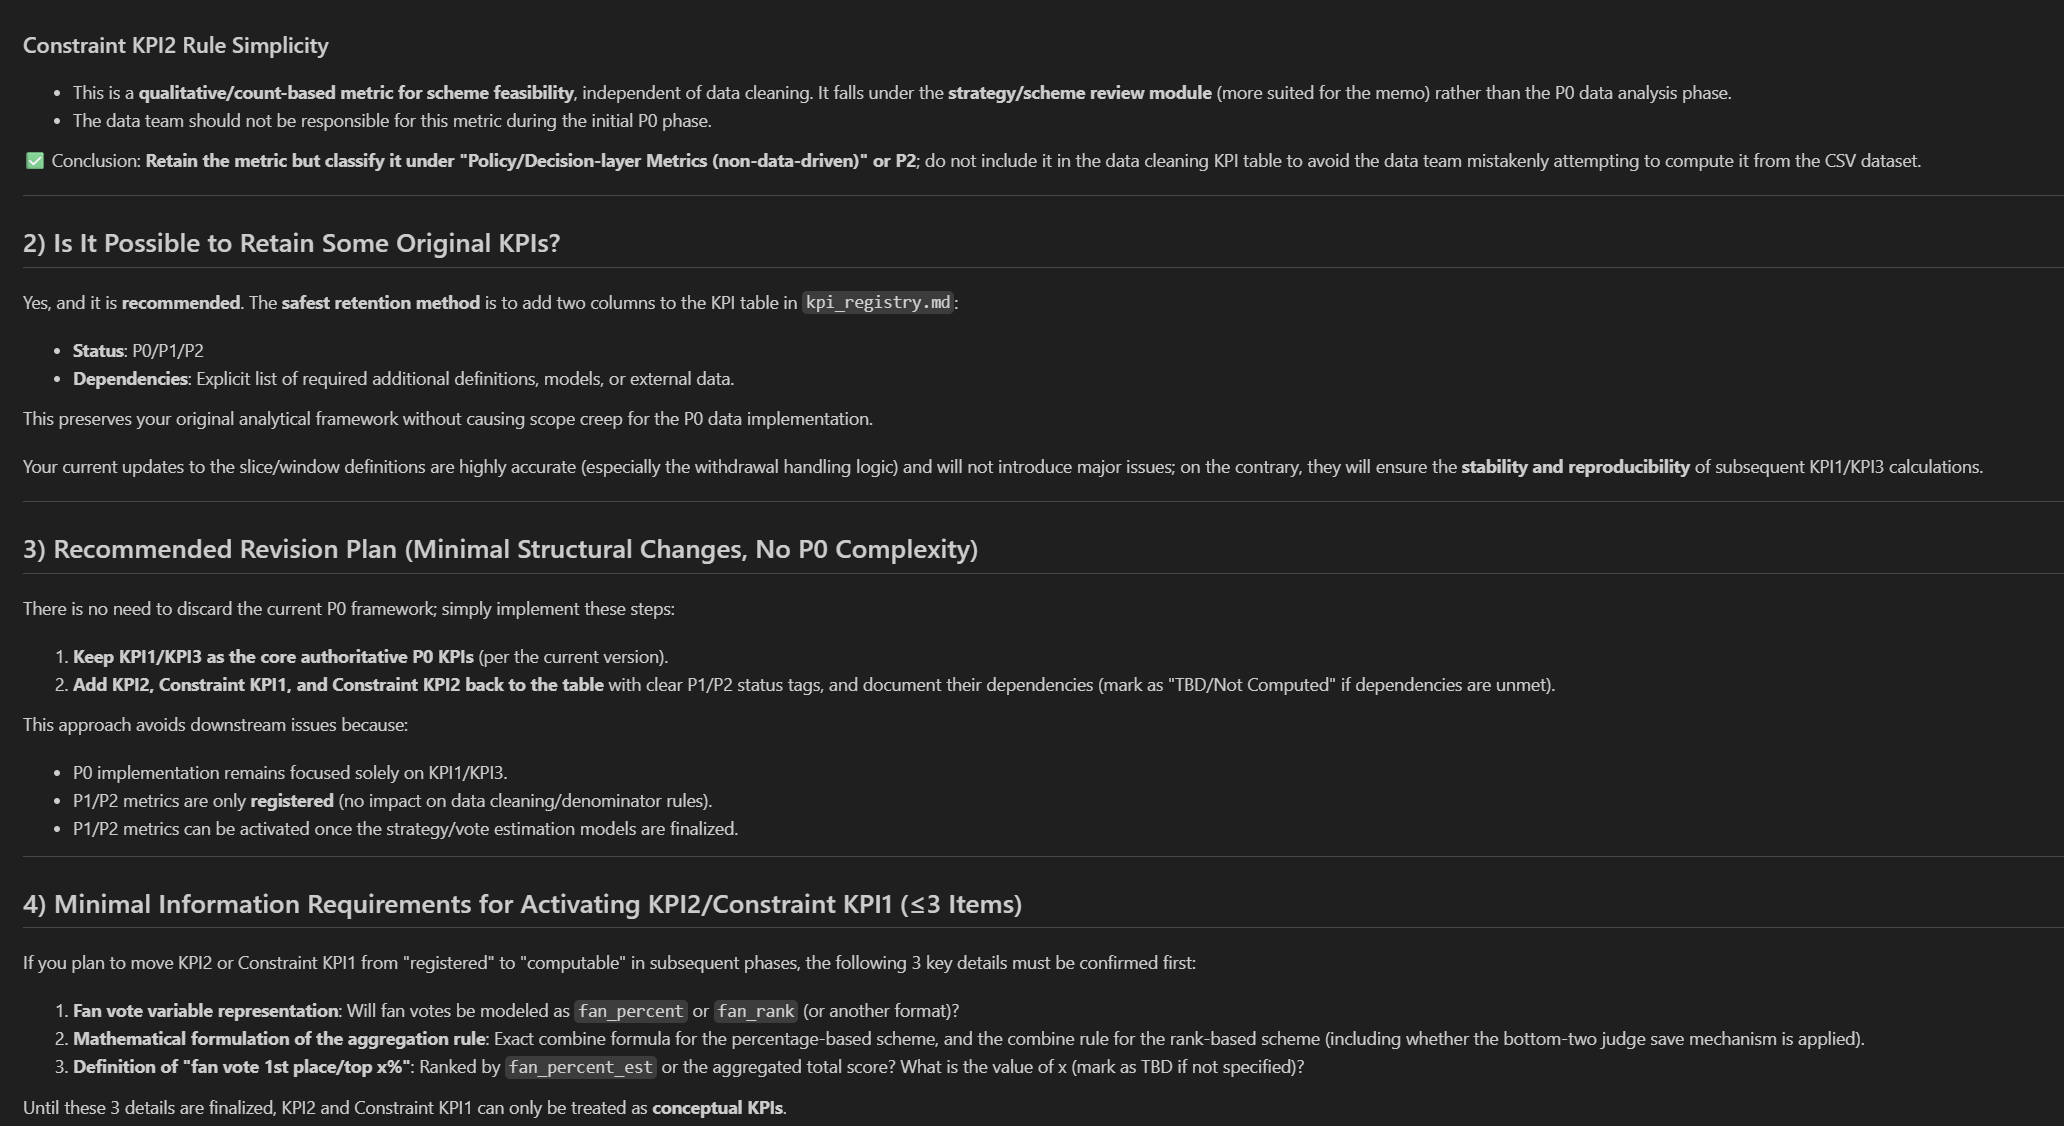
\includegraphics[width=0.9\linewidth]{report_on_use_of_ai/pho/93.png}
  \caption{ChatGPT Query 9 Output Screenshot}
  \label{fig:chatgpt_query_9_output2}
\end{figure}


\textbf{\href{https://github.com/charles65536/model2026-2/blob/main/report_on_use_of_ai/chatgpt_10_input_and_output.md}{ChatGPT Query 10:}}\\
\textbf{Input:}

\begin{figure}[H]
  \centering
  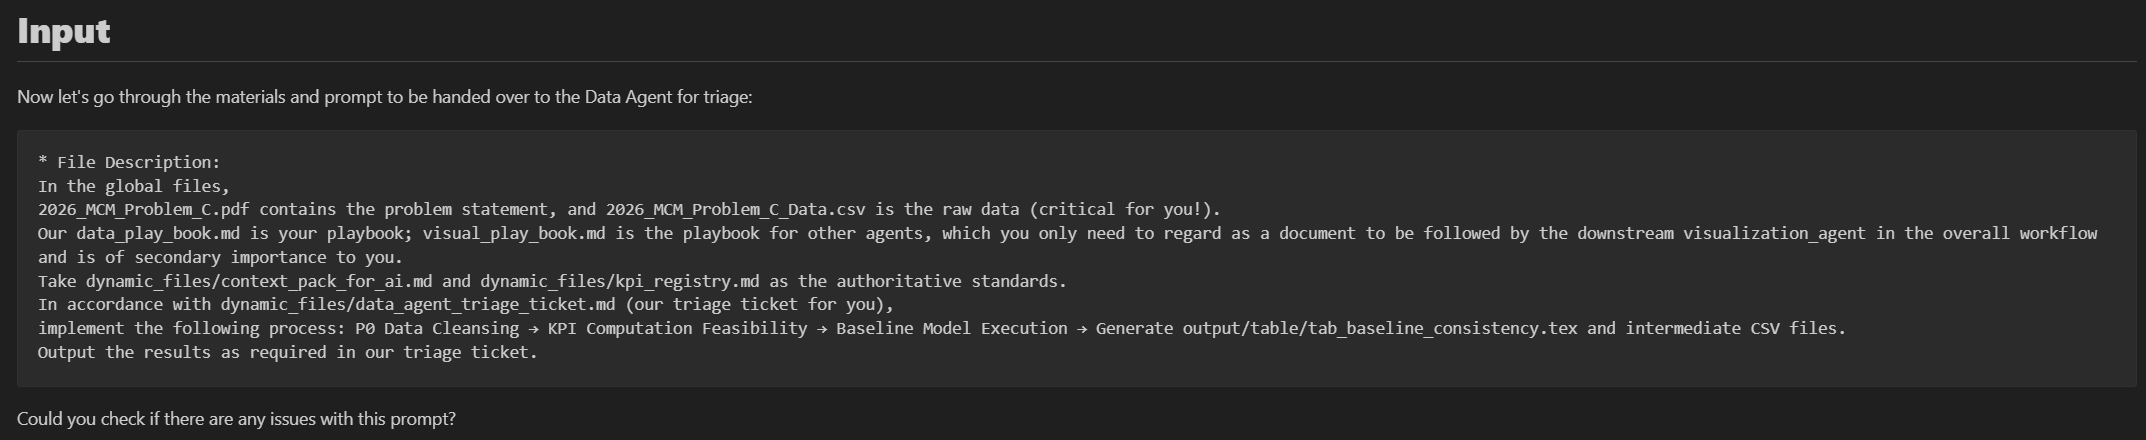
\includegraphics[width=0.9\linewidth]{report_on_use_of_ai/pho/101.png}
  \caption{ChatGPT Query 10 Input Screenshot}
  \label{fig:chatgpt_query_10_input}
\end{figure}

\textbf{Output:}
\begin{figure}[H]
  \centering
  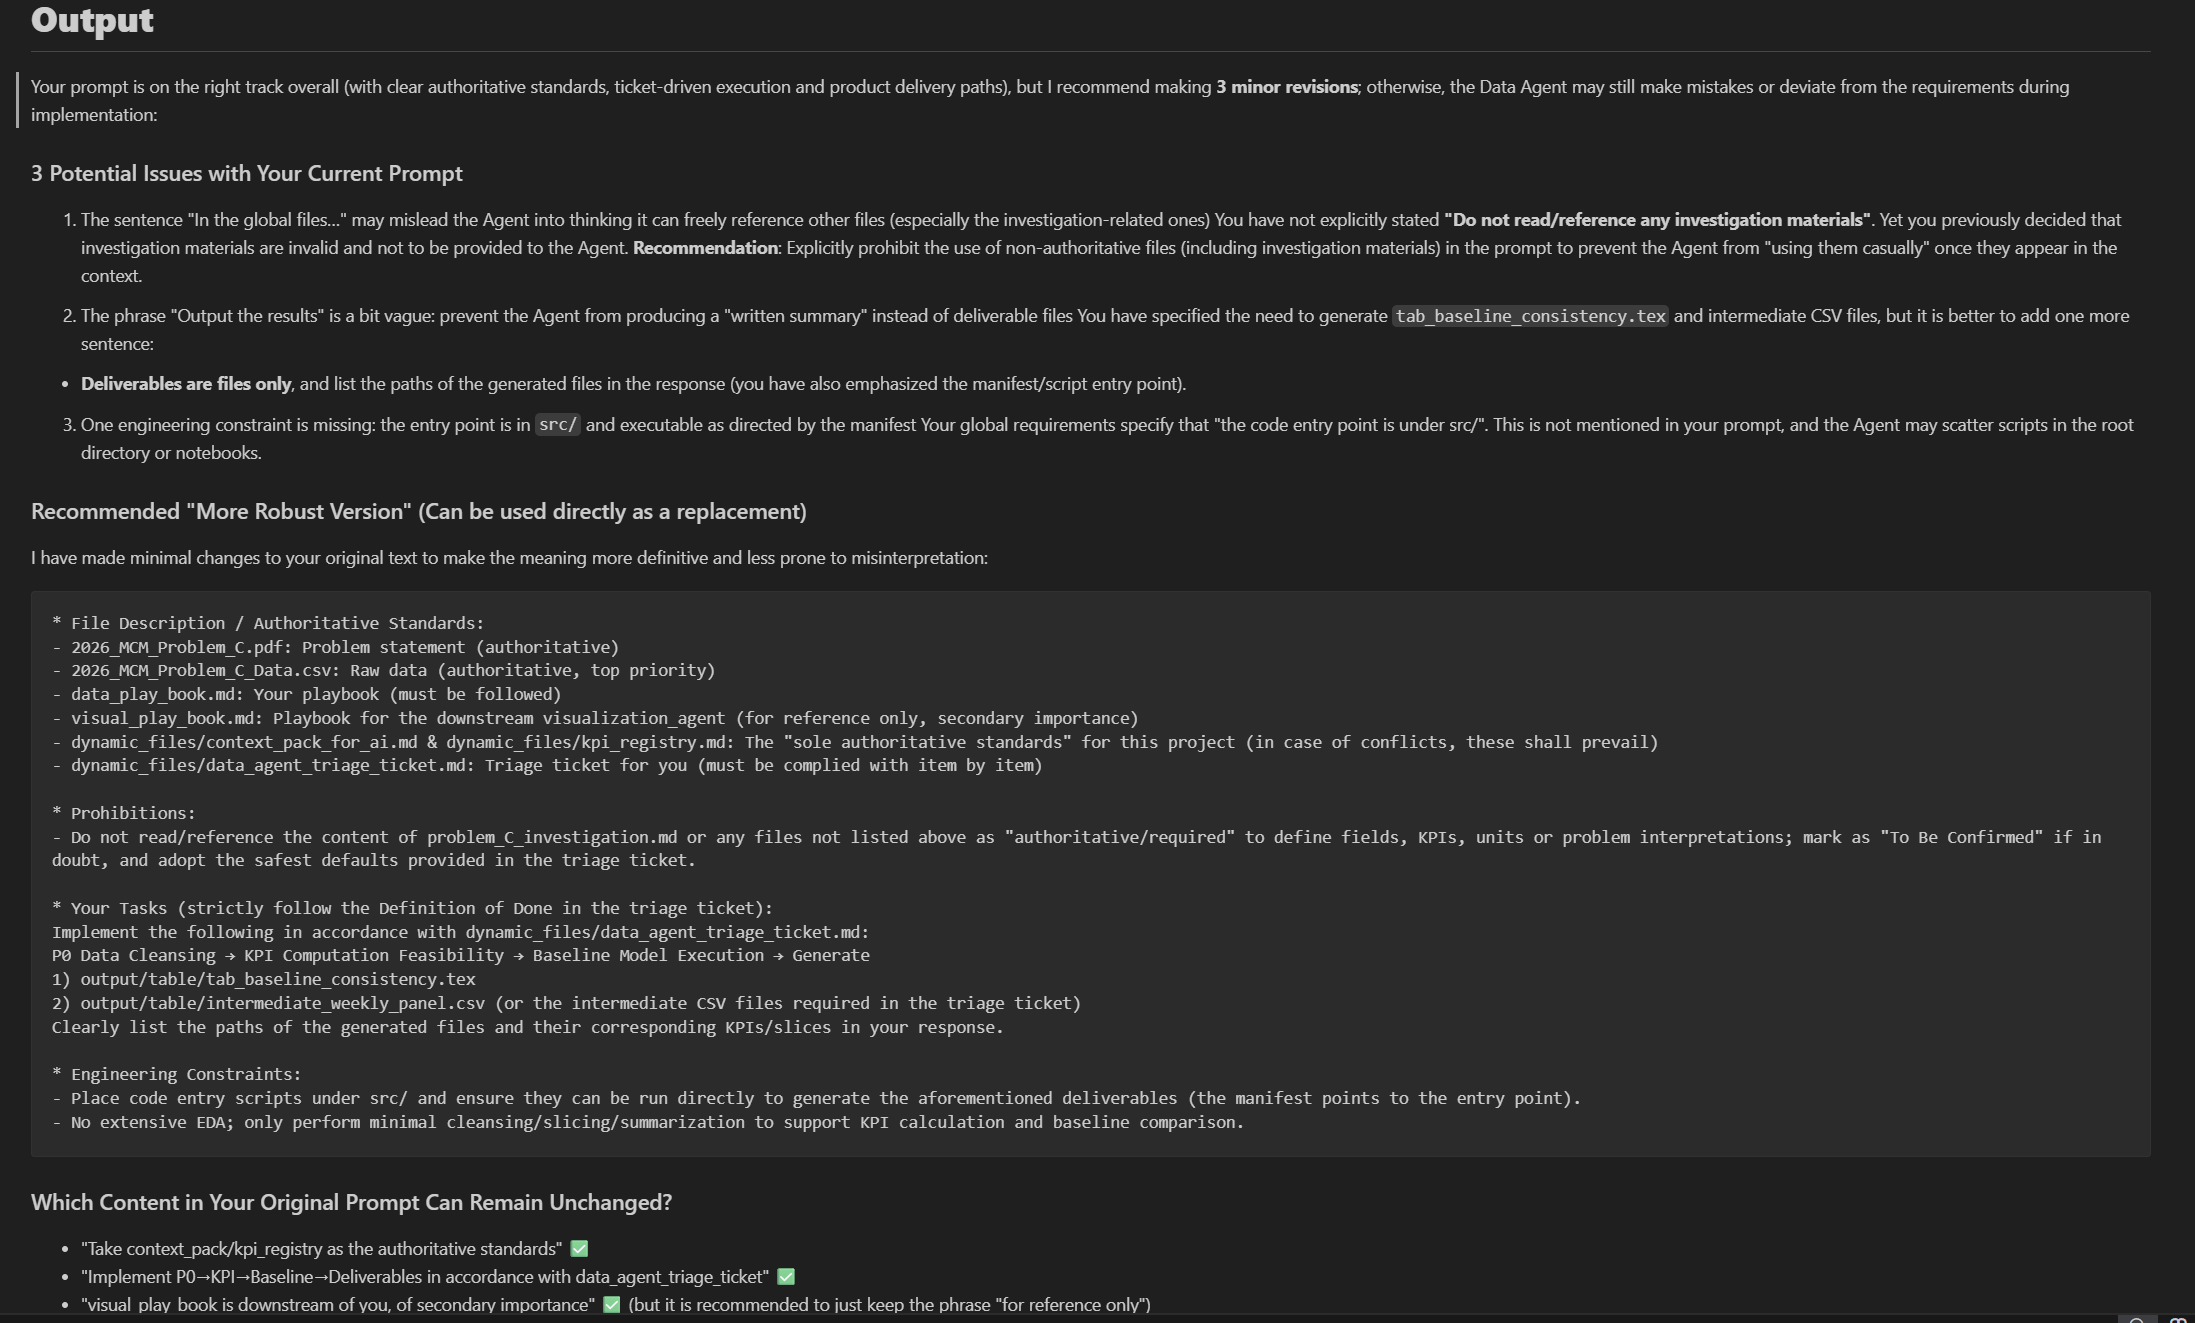
\includegraphics[width=0.9\linewidth]{report_on_use_of_ai/pho/102.png}
  \caption{ChatGPT Query 10 Output Screenshot}
  \label{fig:chatgpt_query_10_output}
\end{figure}

\begin{figure}[H]
  \centering
  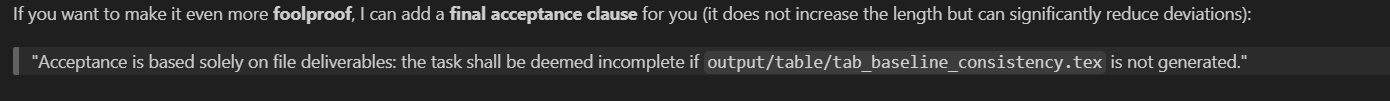
\includegraphics[width=0.9\linewidth]{report_on_use_of_ai/pho/103.png}
  \caption{ChatGPT Query 10 Output Screenshot}
  \label{fig:chatgpt_query_10_output2}
\end{figure}


\textbf{\href{https://github.com/charles65536/model2026-2/blob/main/report_on_use_of_ai/chatgpt_11_input_and_output.md}{ChatGPT Query 11:}}\\
\textbf{Input:}

\begin{figure}[H]
  \centering
  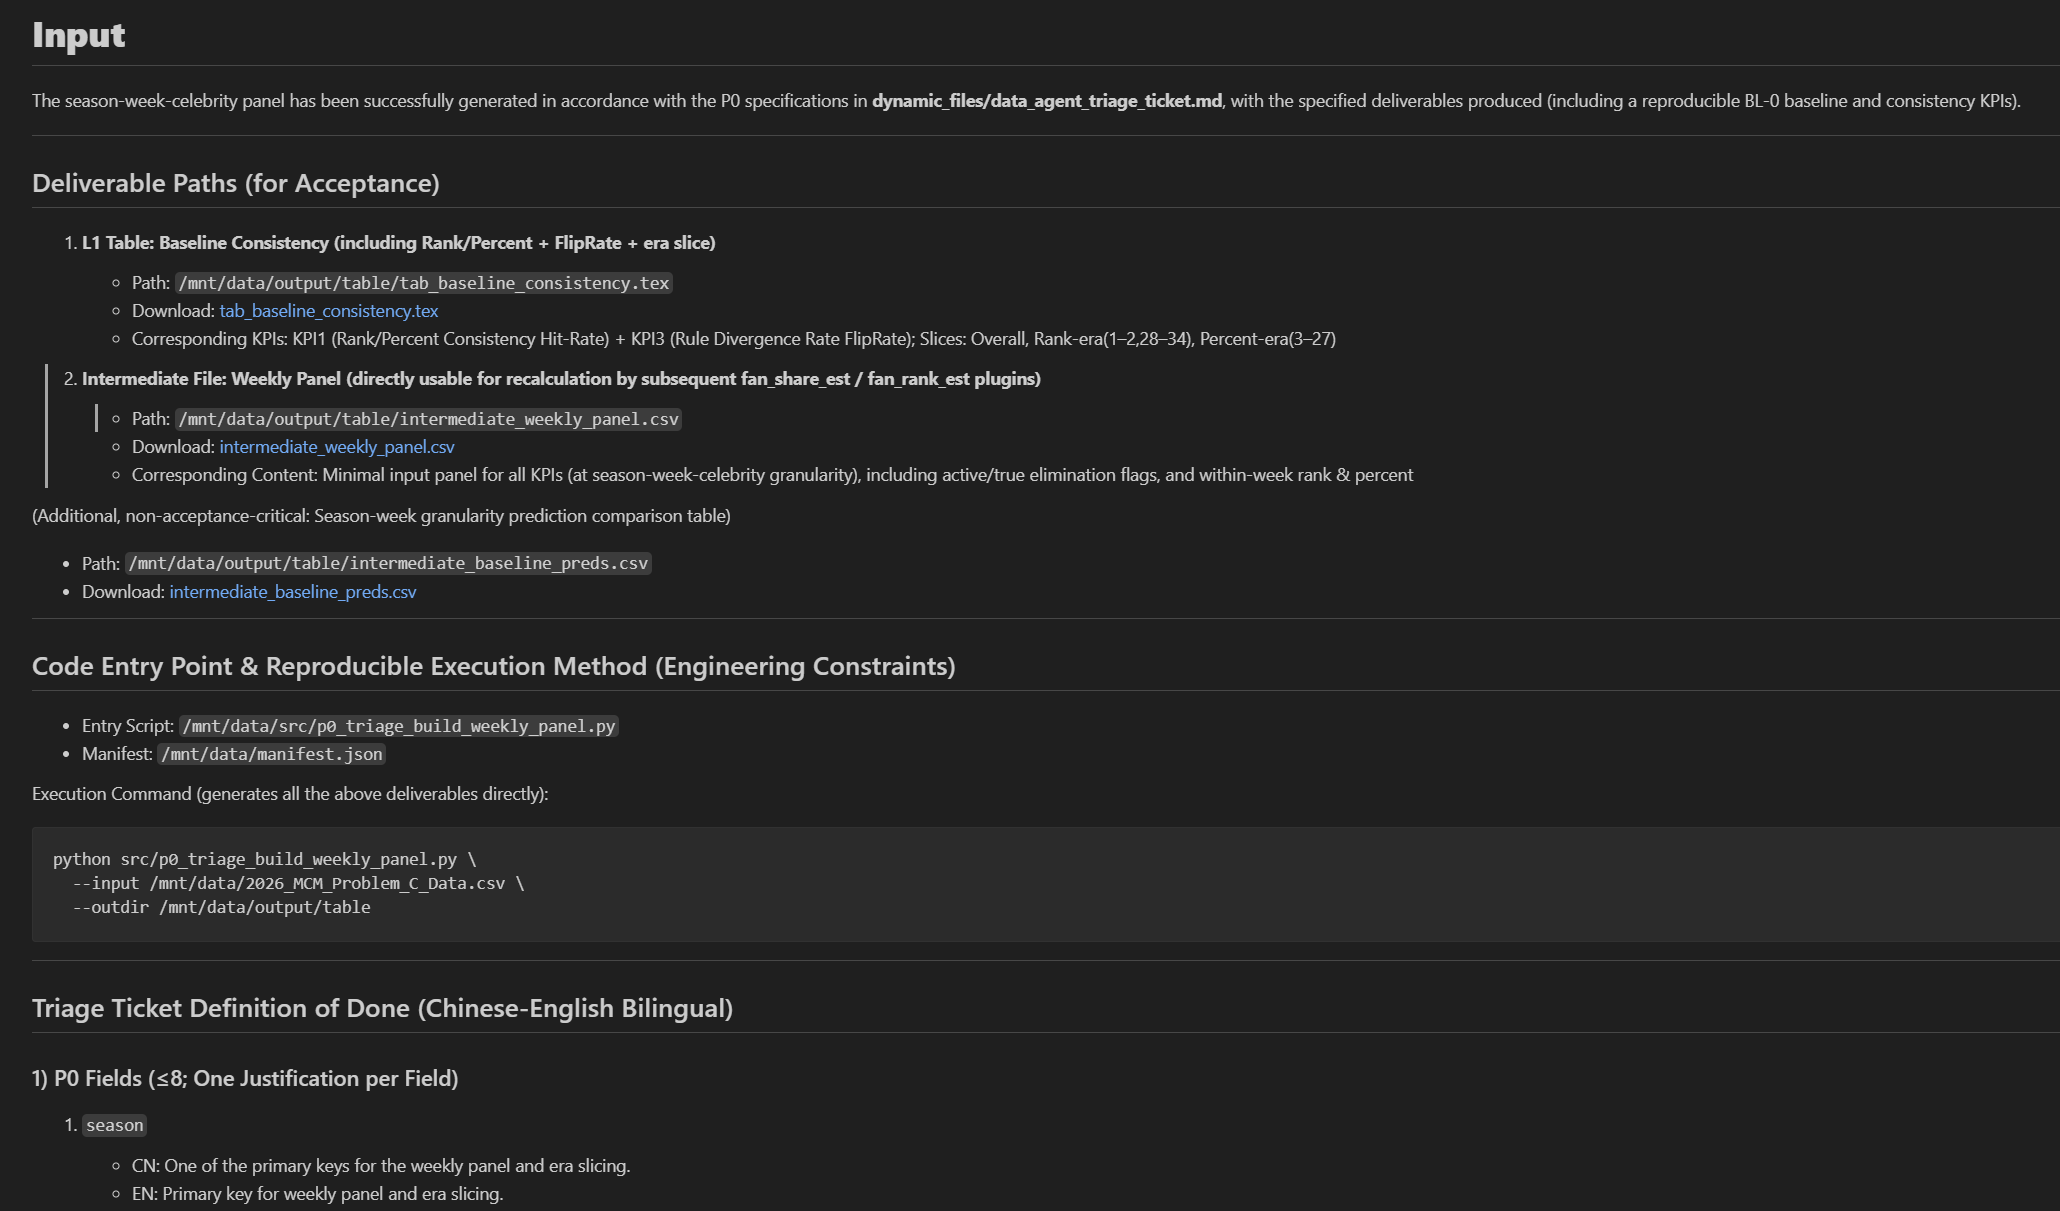
\includegraphics[width=0.9\linewidth]{report_on_use_of_ai/pho/111.png}
  \caption{ChatGPT Query 11 Input Screenshot}
  \label{fig:chatgpt_query_11_input}
\end{figure}

\textbf{Output:}
\begin{figure}[H]
  \centering
  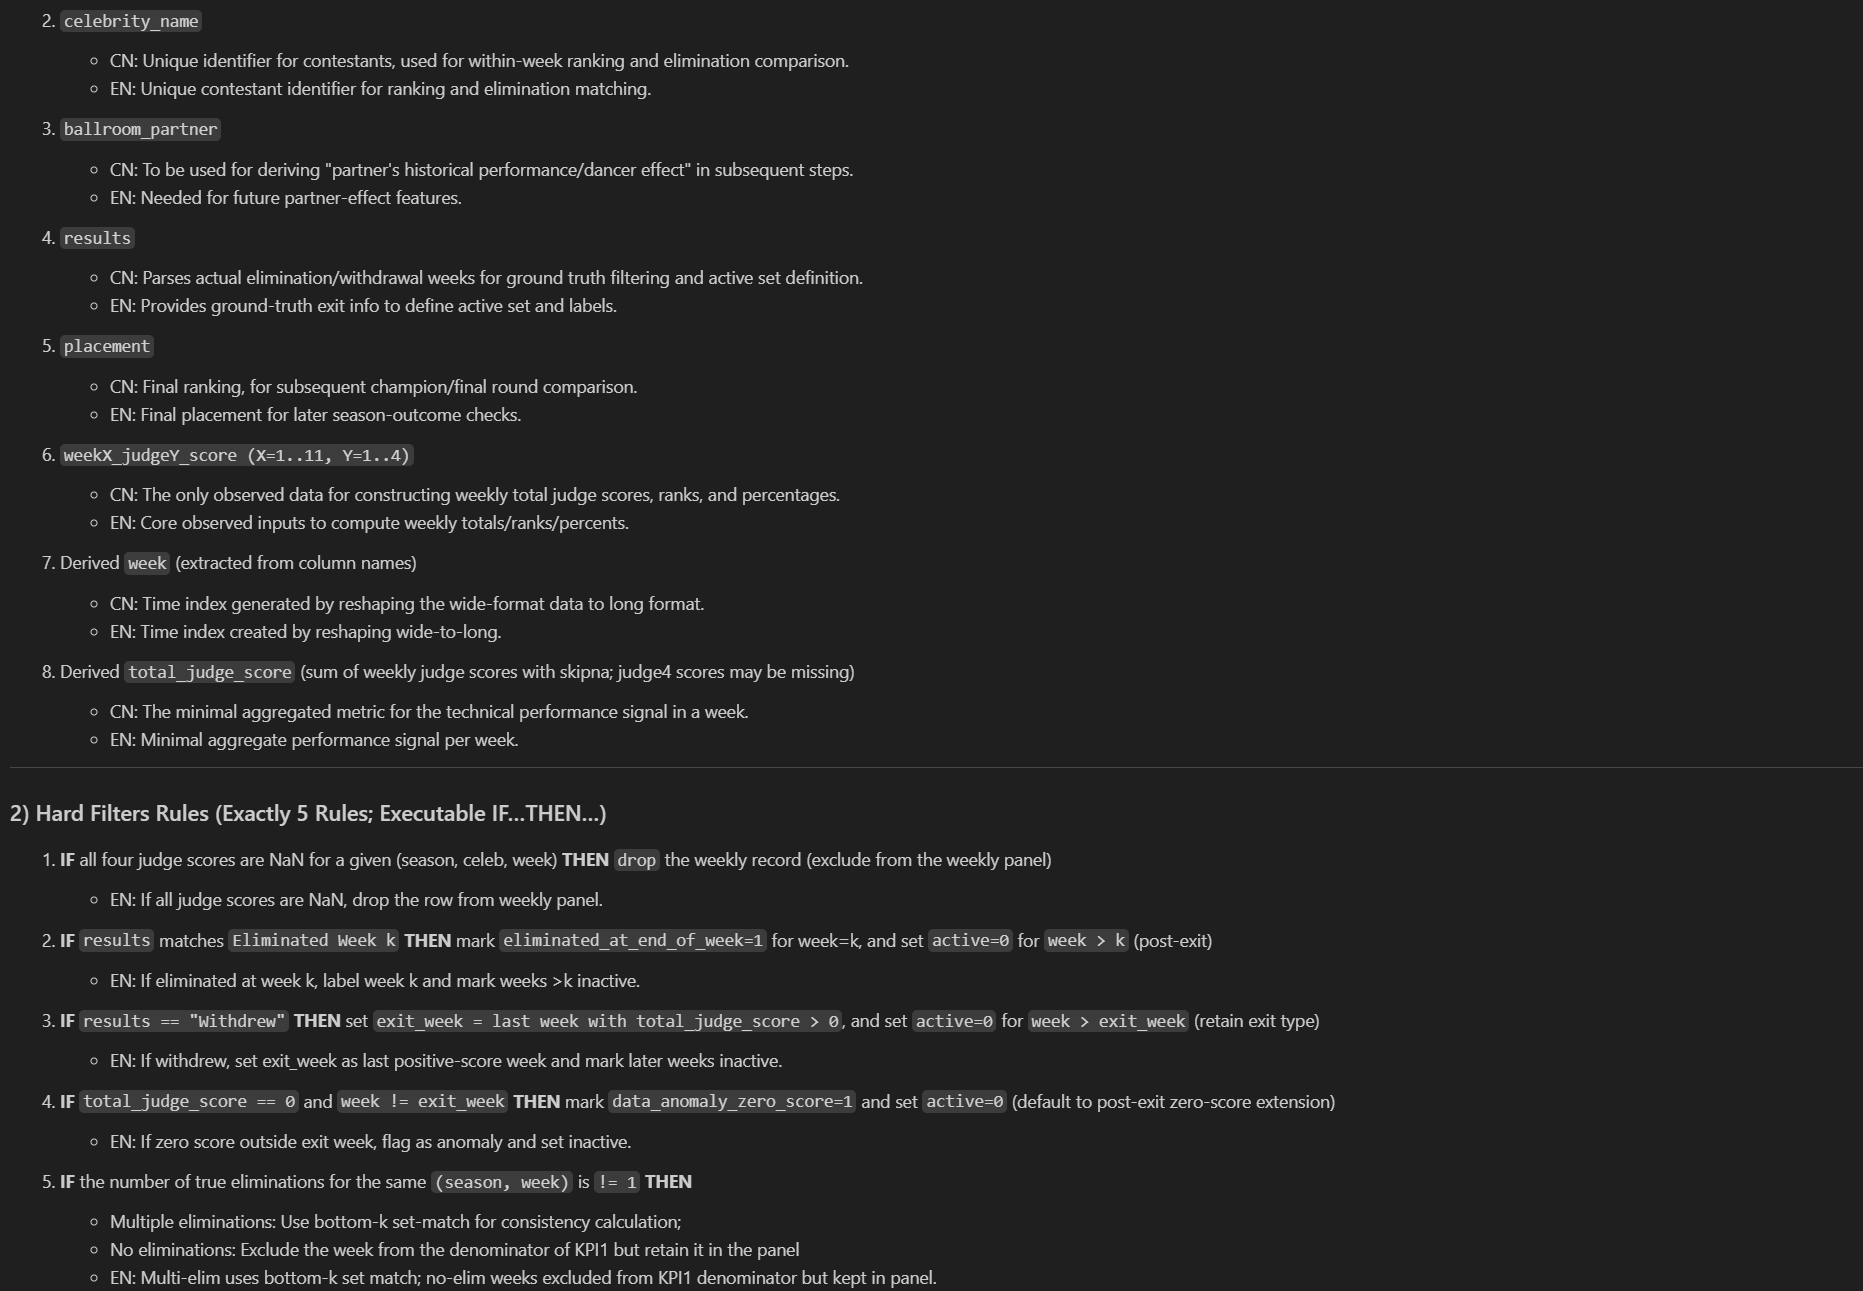
\includegraphics[width=0.9\linewidth]{report_on_use_of_ai/pho/112.png}
  \caption{ChatGPT Query 11 Output Screenshot}
  \label{fig:chatgpt_query_11_output}
\end{figure}
\begin{figure}[H]
  \centering
  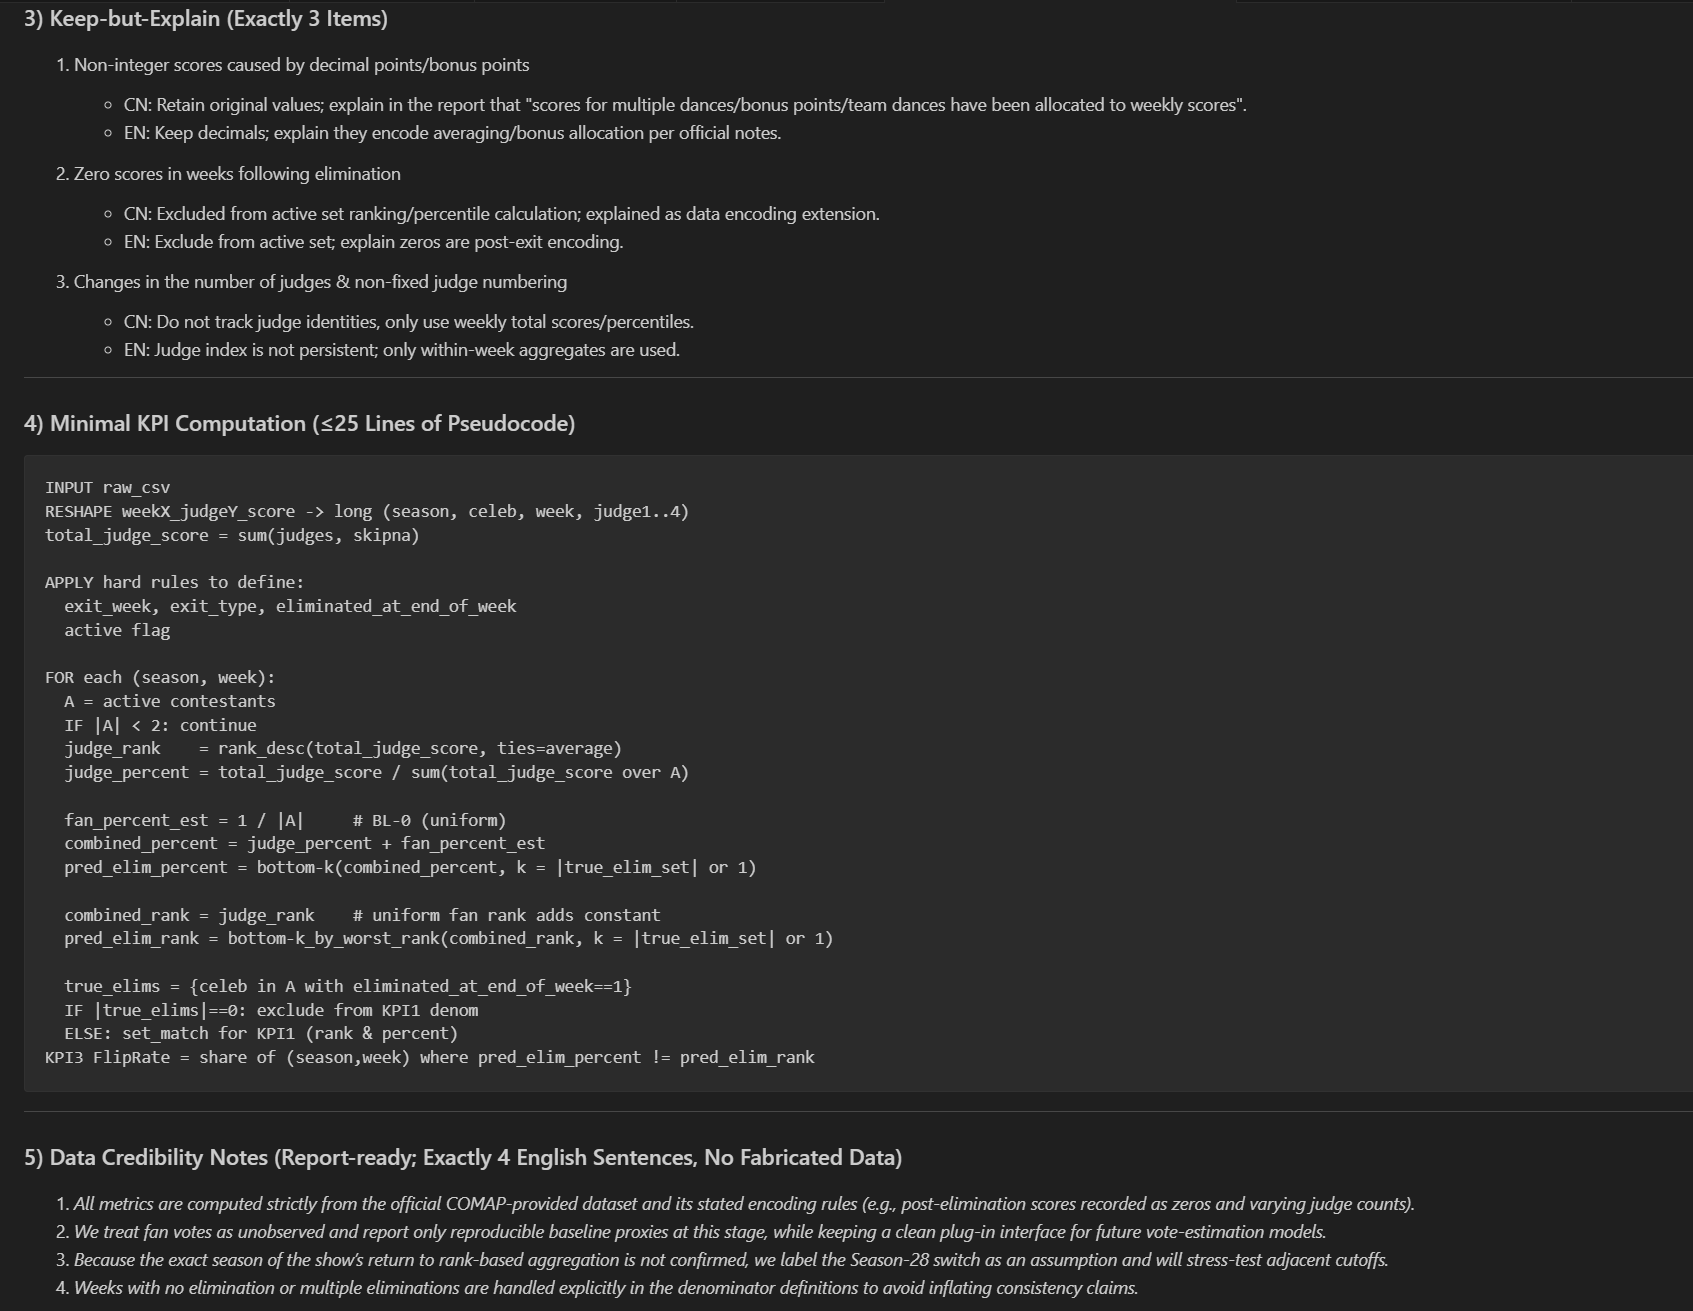
\includegraphics[width=0.9\linewidth]{report_on_use_of_ai/pho/113.png}
  \caption{ChatGPT Query 11 Output Screenshot}
  \label{fig:chatgpt_query_11_output2}
\end{figure}




\textbf{\href{https://github.com/charles65536/model2026-2/blob/main/report_on_use_of_ai/chatgpt_12_input_and_output.md}{ChatGPT Query 12:}}\\
\textbf{Input:}
\begin{figure}[H]
  \centering
  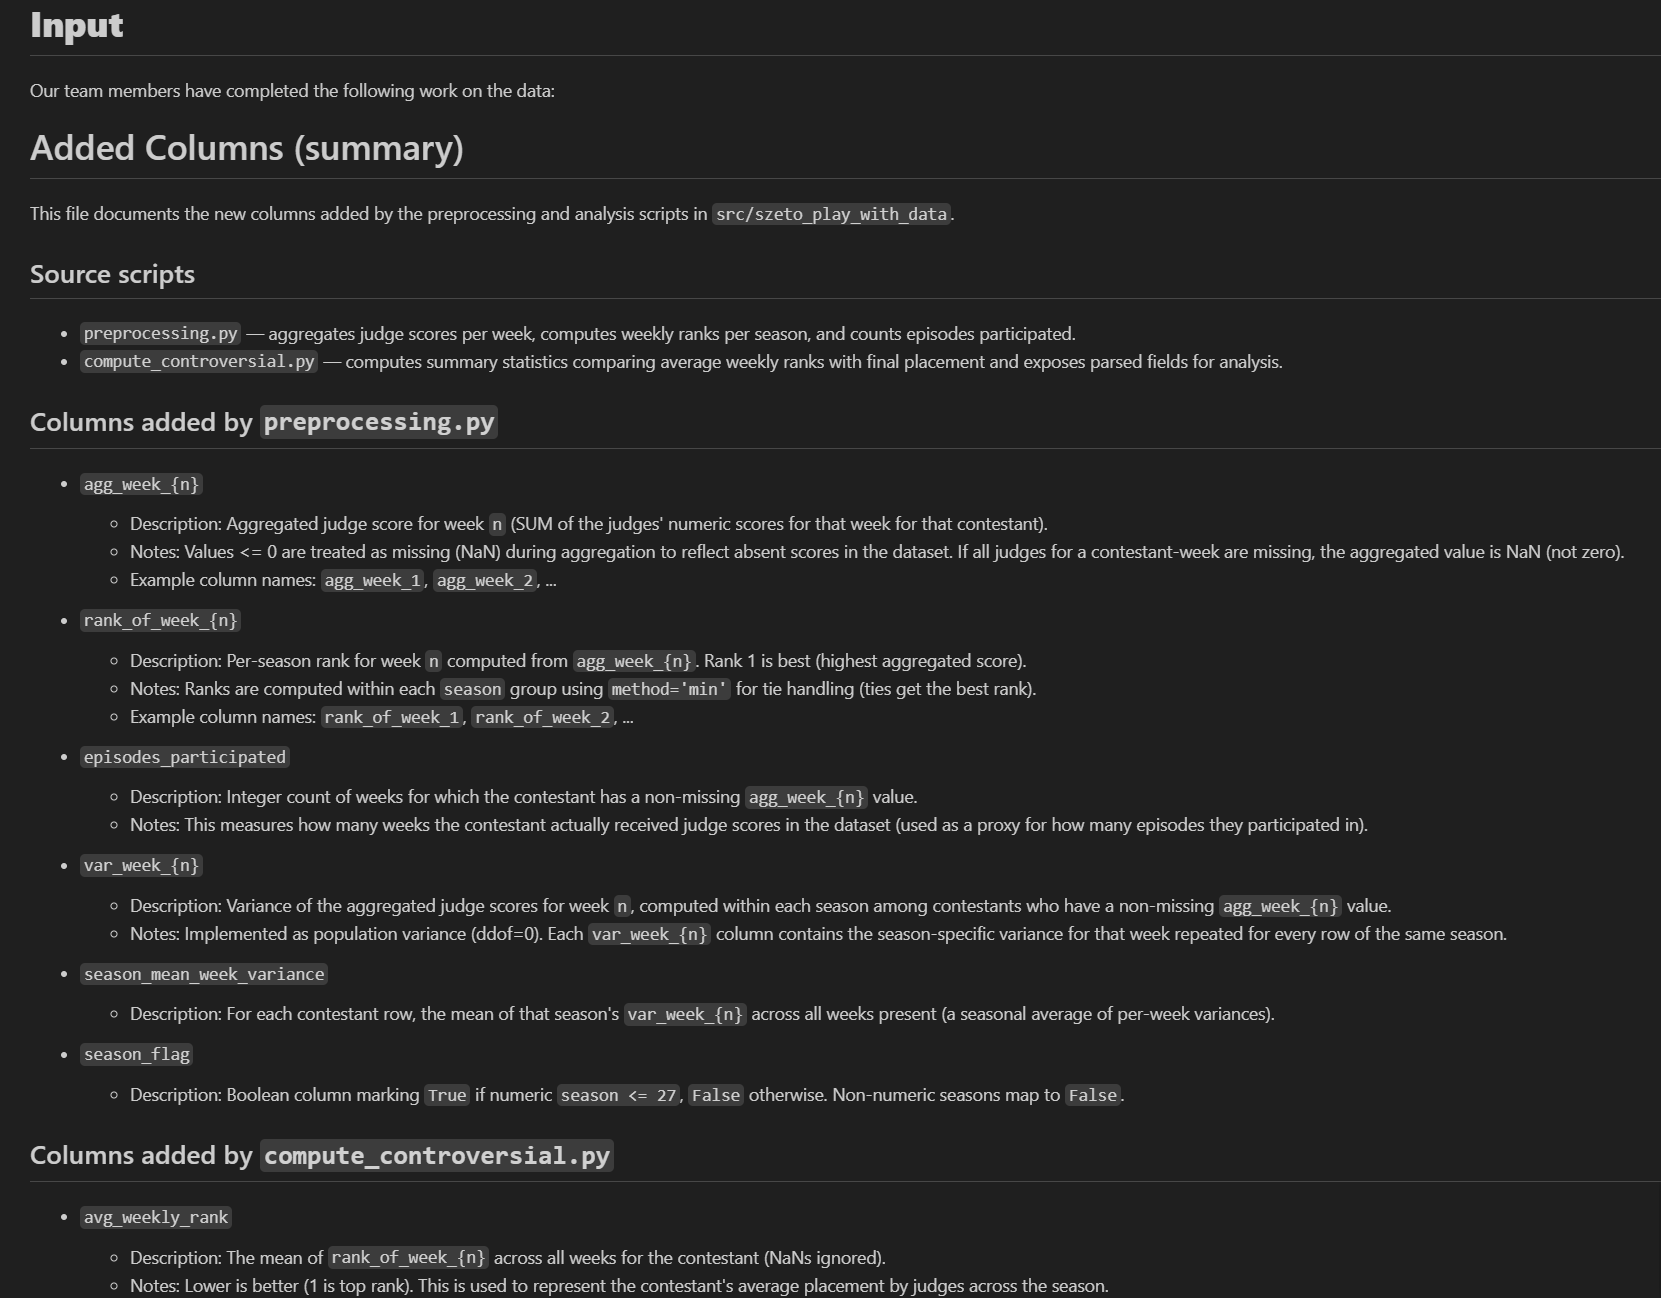
\includegraphics[width=0.9\linewidth]{report_on_use_of_ai/pho/121.png}
  \caption{ChatGPT Query 12 Input Screenshot}
  \label{fig:chatgpt_query_12_input}
\end{figure}

\textbf{Output:}
\begin{figure}[H]
  \centering
  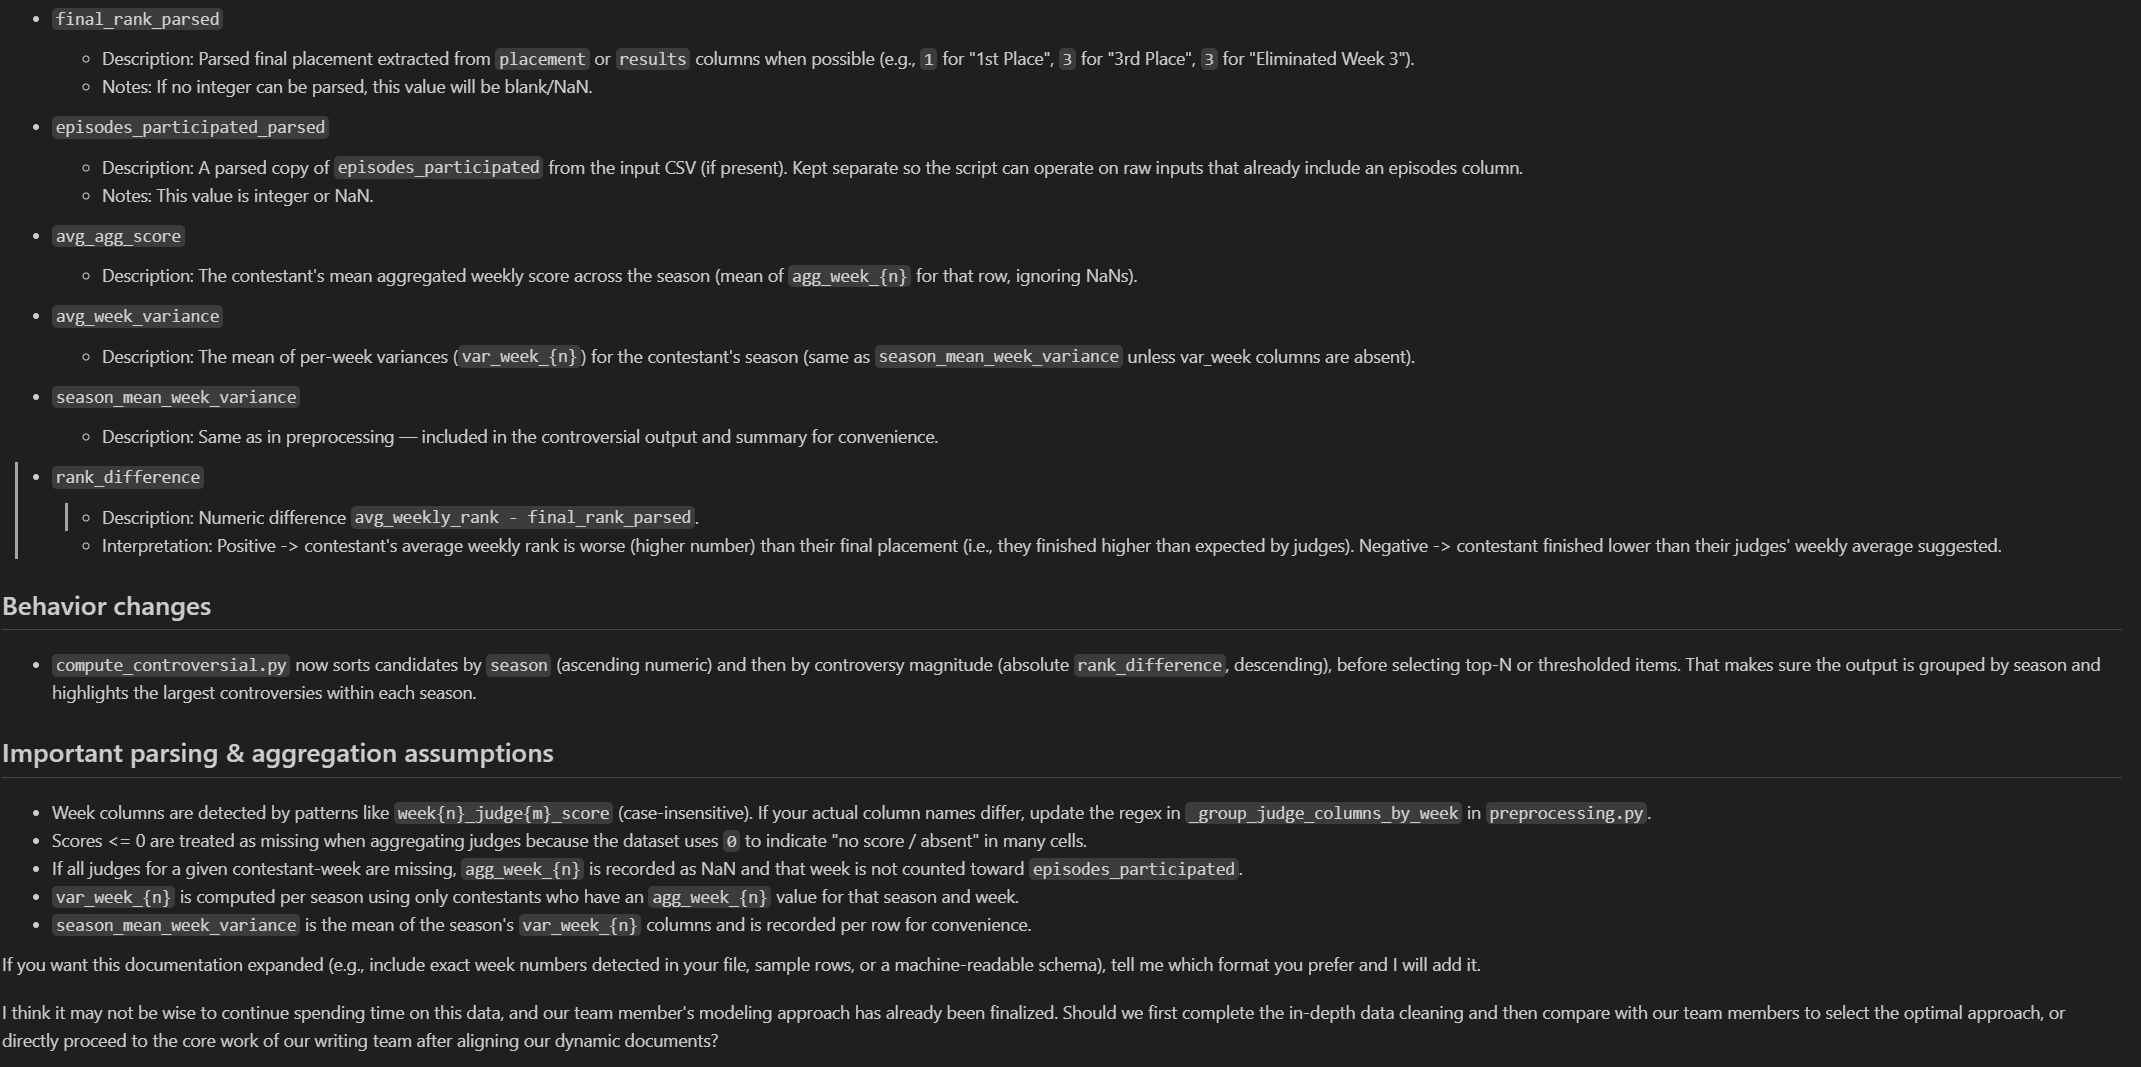
\includegraphics[width=0.9\linewidth]{report_on_use_of_ai/pho/122.png}
  \caption{ChatGPT Query 12 Output Screenshot}
  \label{fig:chatgpt_query_12_output}
\end{figure}
\begin{figure}[H]
  \centering
  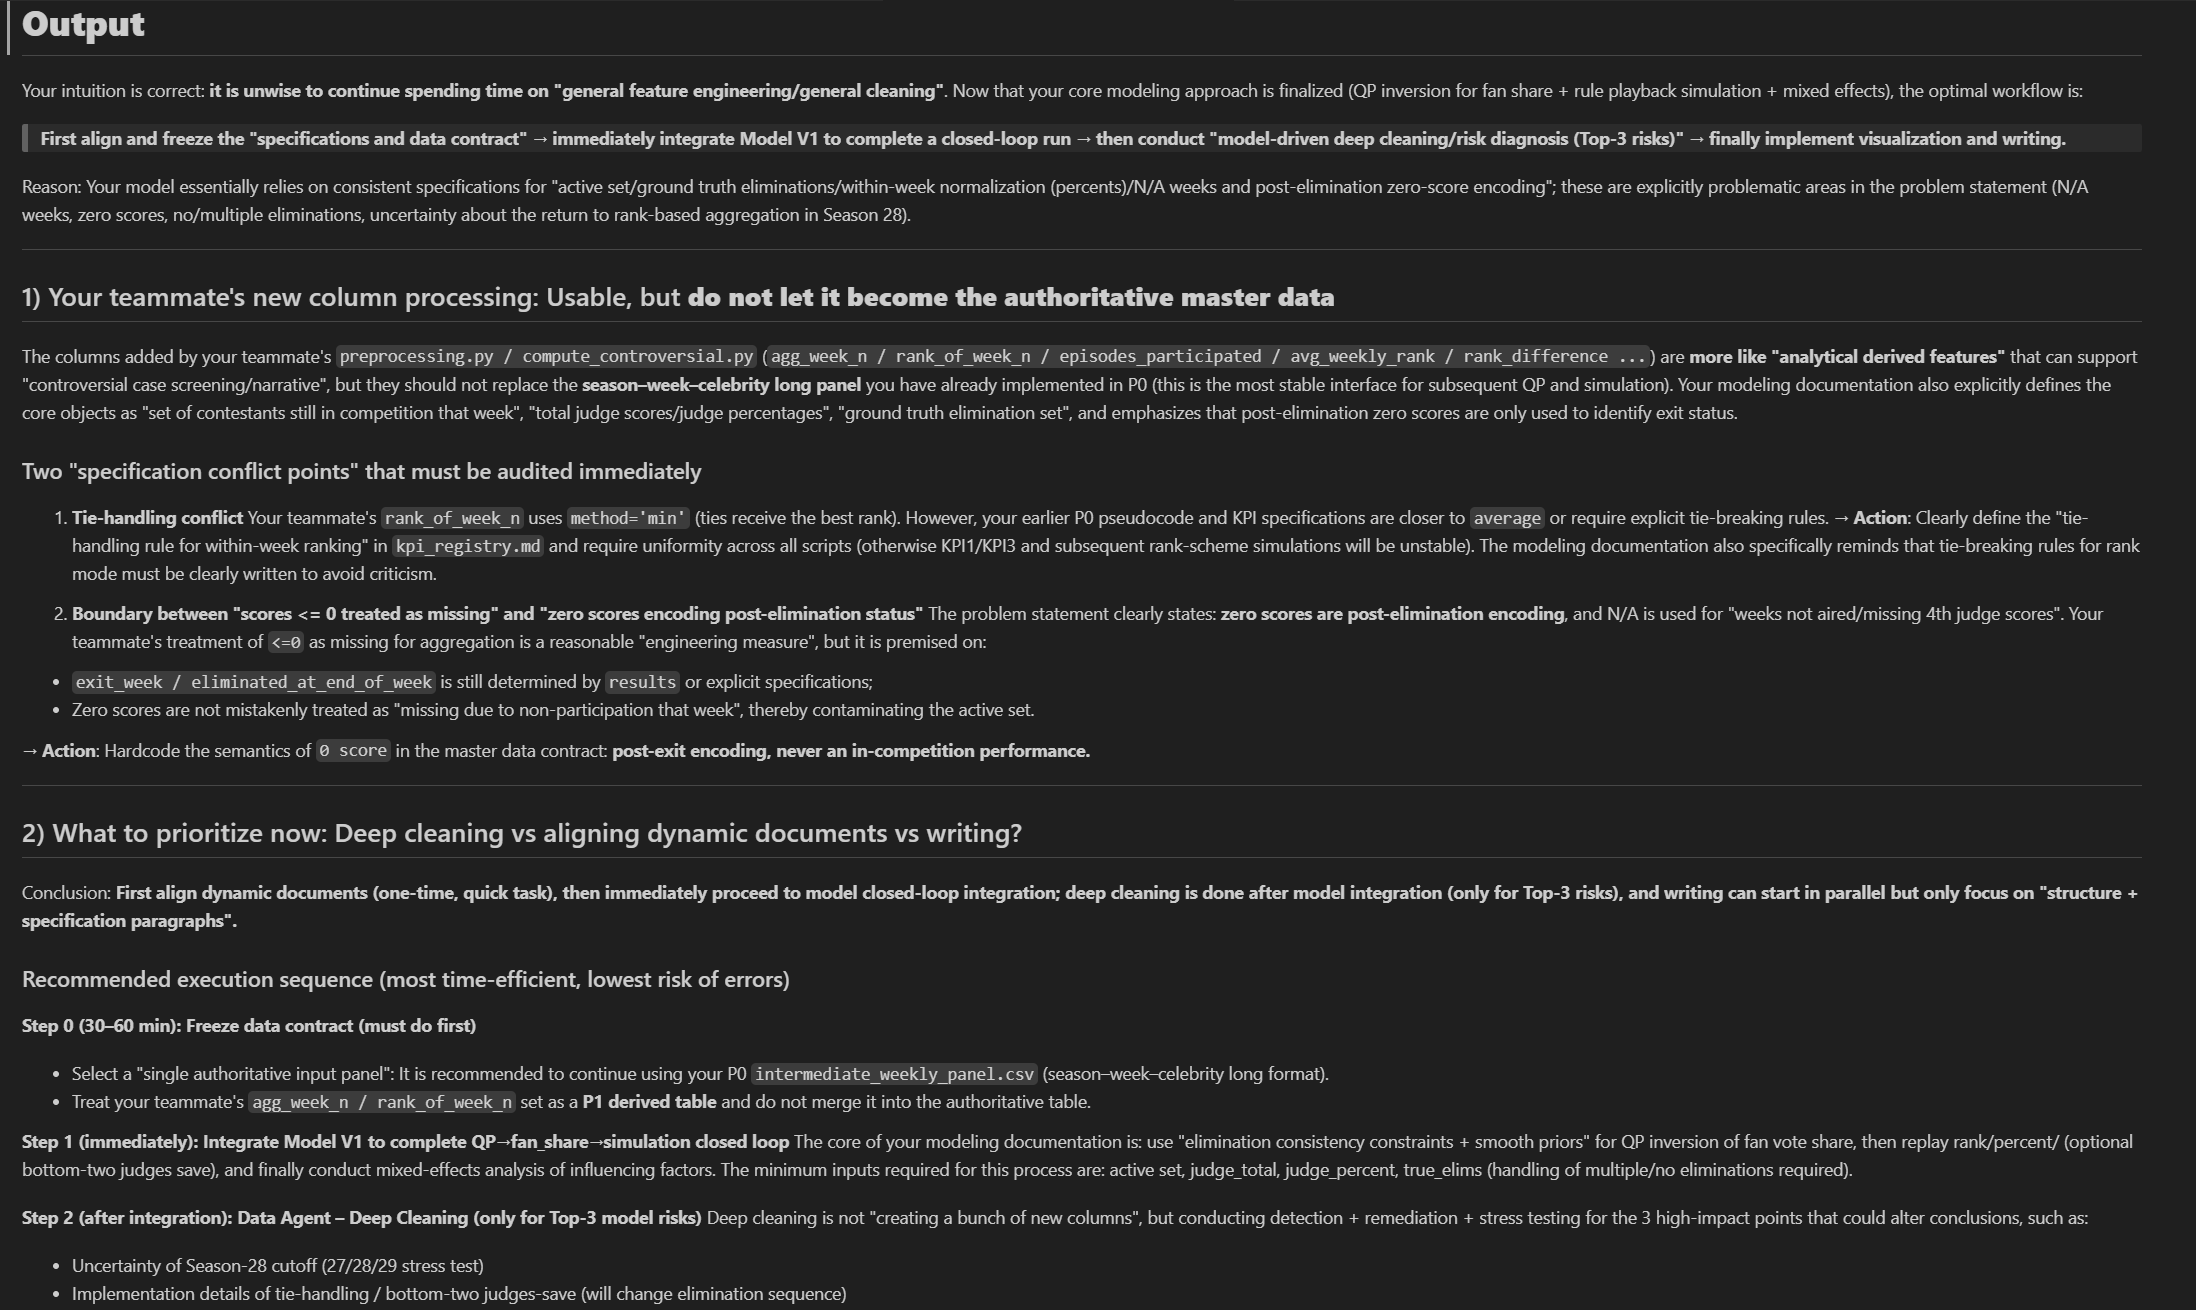
\includegraphics[width=0.9\linewidth]{report_on_use_of_ai/pho/123.png}
  \caption{ChatGPT Query 12 Output Screenshot}
  \label{fig:chatgpt_query_12_output_2}
\end{figure}
\begin{figure}[H]
  \centering
  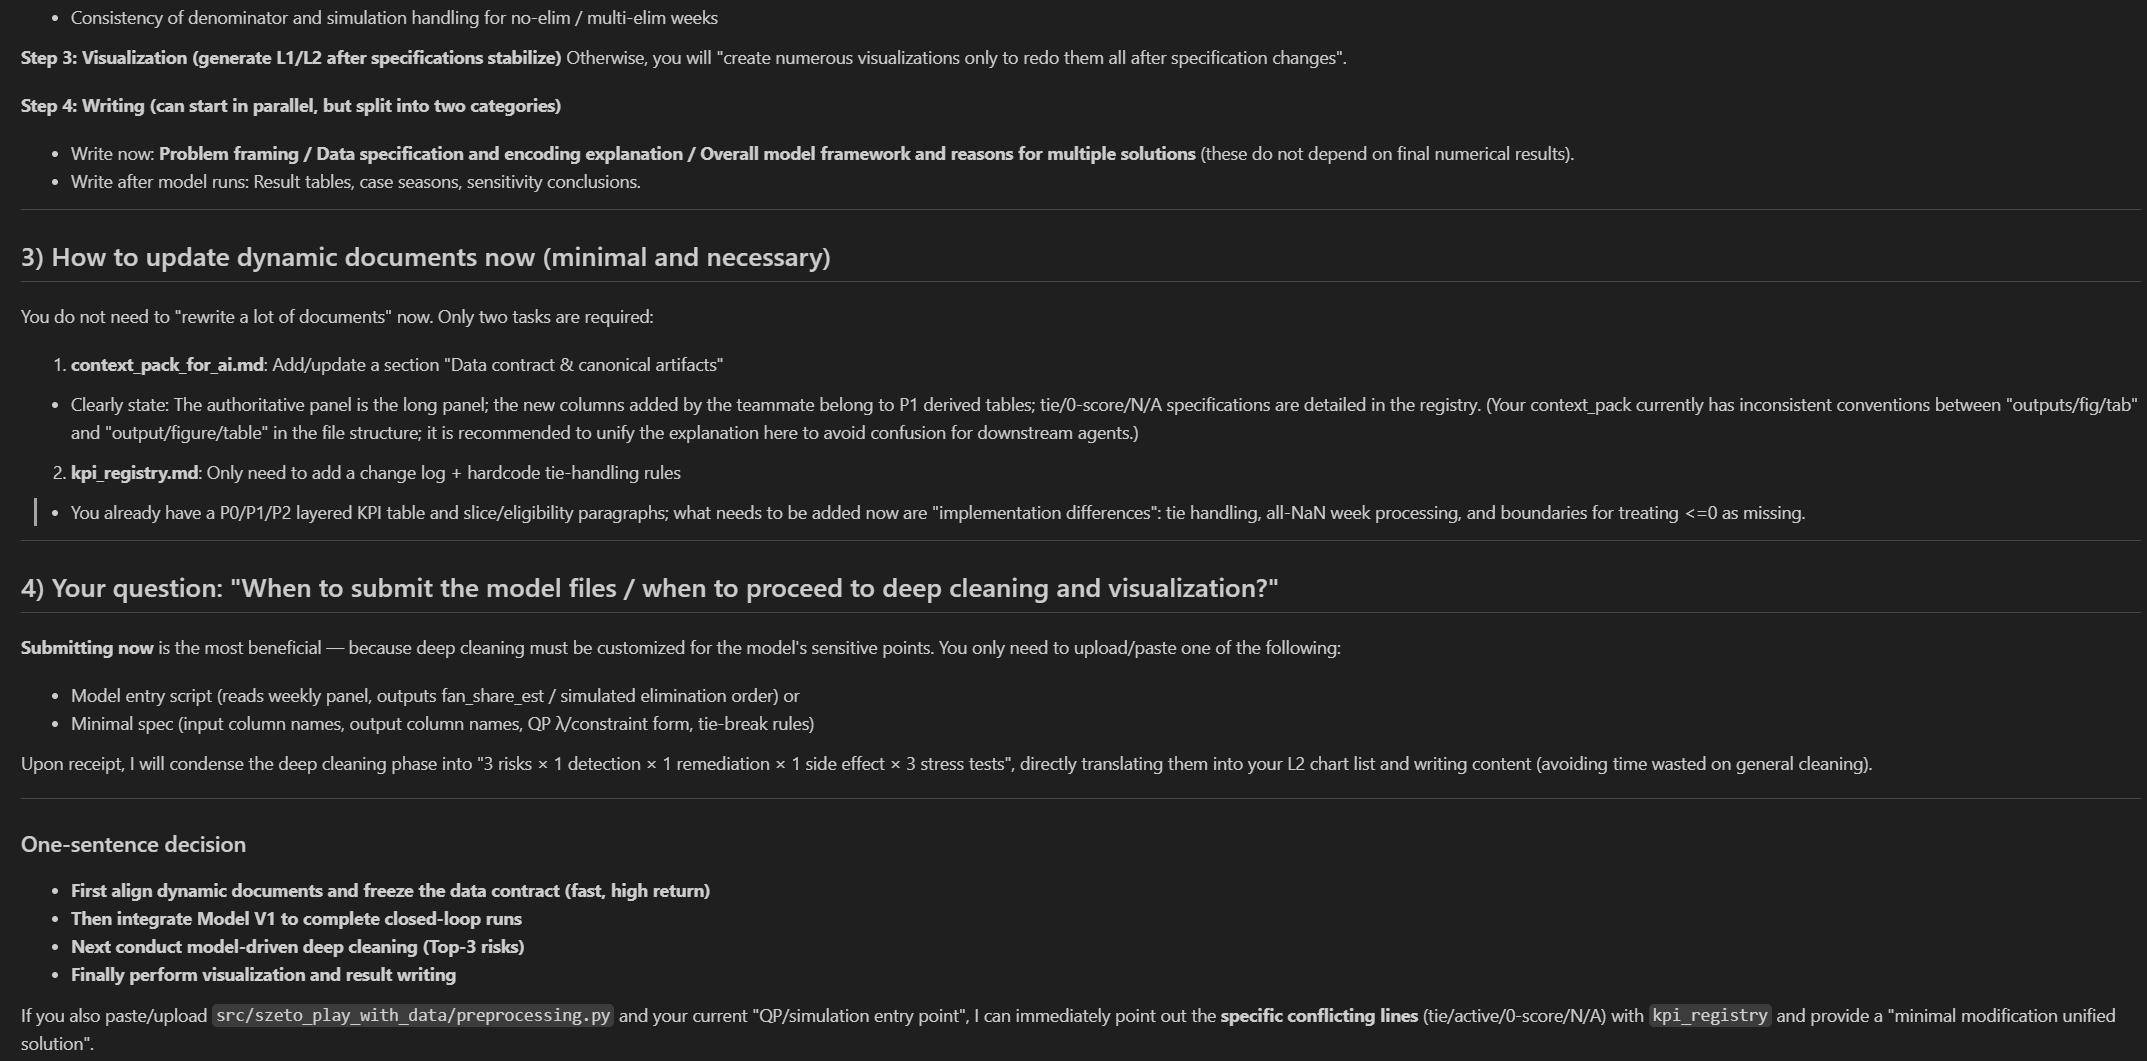
\includegraphics[width=0.9\linewidth]{report_on_use_of_ai/pho/124.png}
  \caption{ChatGPT Query 12 Output Screenshot}
  \label{fig:chatgpt_query_12_output_3}
\end{figure}




\textbf{\href{https://github.com/charles65536/model2026-2/blob/main/report_on_use_of_ai/chatgpt_13_input_and_output.md}{ChatGPT Query 13:}}\\
\textbf{Input:}
So let me sort out what we need to do now:
First step: Align our specifications. You mentioned freezing and sticking to our core data pipeline, but actually I don't think this is necessary. Because after my teammate makes modifications, they will put their work in their own folder on GitHub, and mine will go into my folder. Even though we're in the same GitHub repository, we can cross-check each other's work later---it'll be like mutual supplementation.
Second step: Integrating Model V1. I don't quite understand this part—does V1 refer to a code file (not a DOCX document) that will make the model we've designed actually run? Is that the right understanding?
Then third step: Conduct in-depth data cleaning, followed by visualization and finalizing the writing. Is this the correct workflow?
I also have another question: Earlier, we identified two risks of inconsistent specifications, right? Well, I suggest we fix these specification inconsistencies first—preferably by modifying the code. I'll send you the code, and could you guide me on exactly what needs to be changed?\\
\textbf{Output:}
\begin{figure}
  \centering
  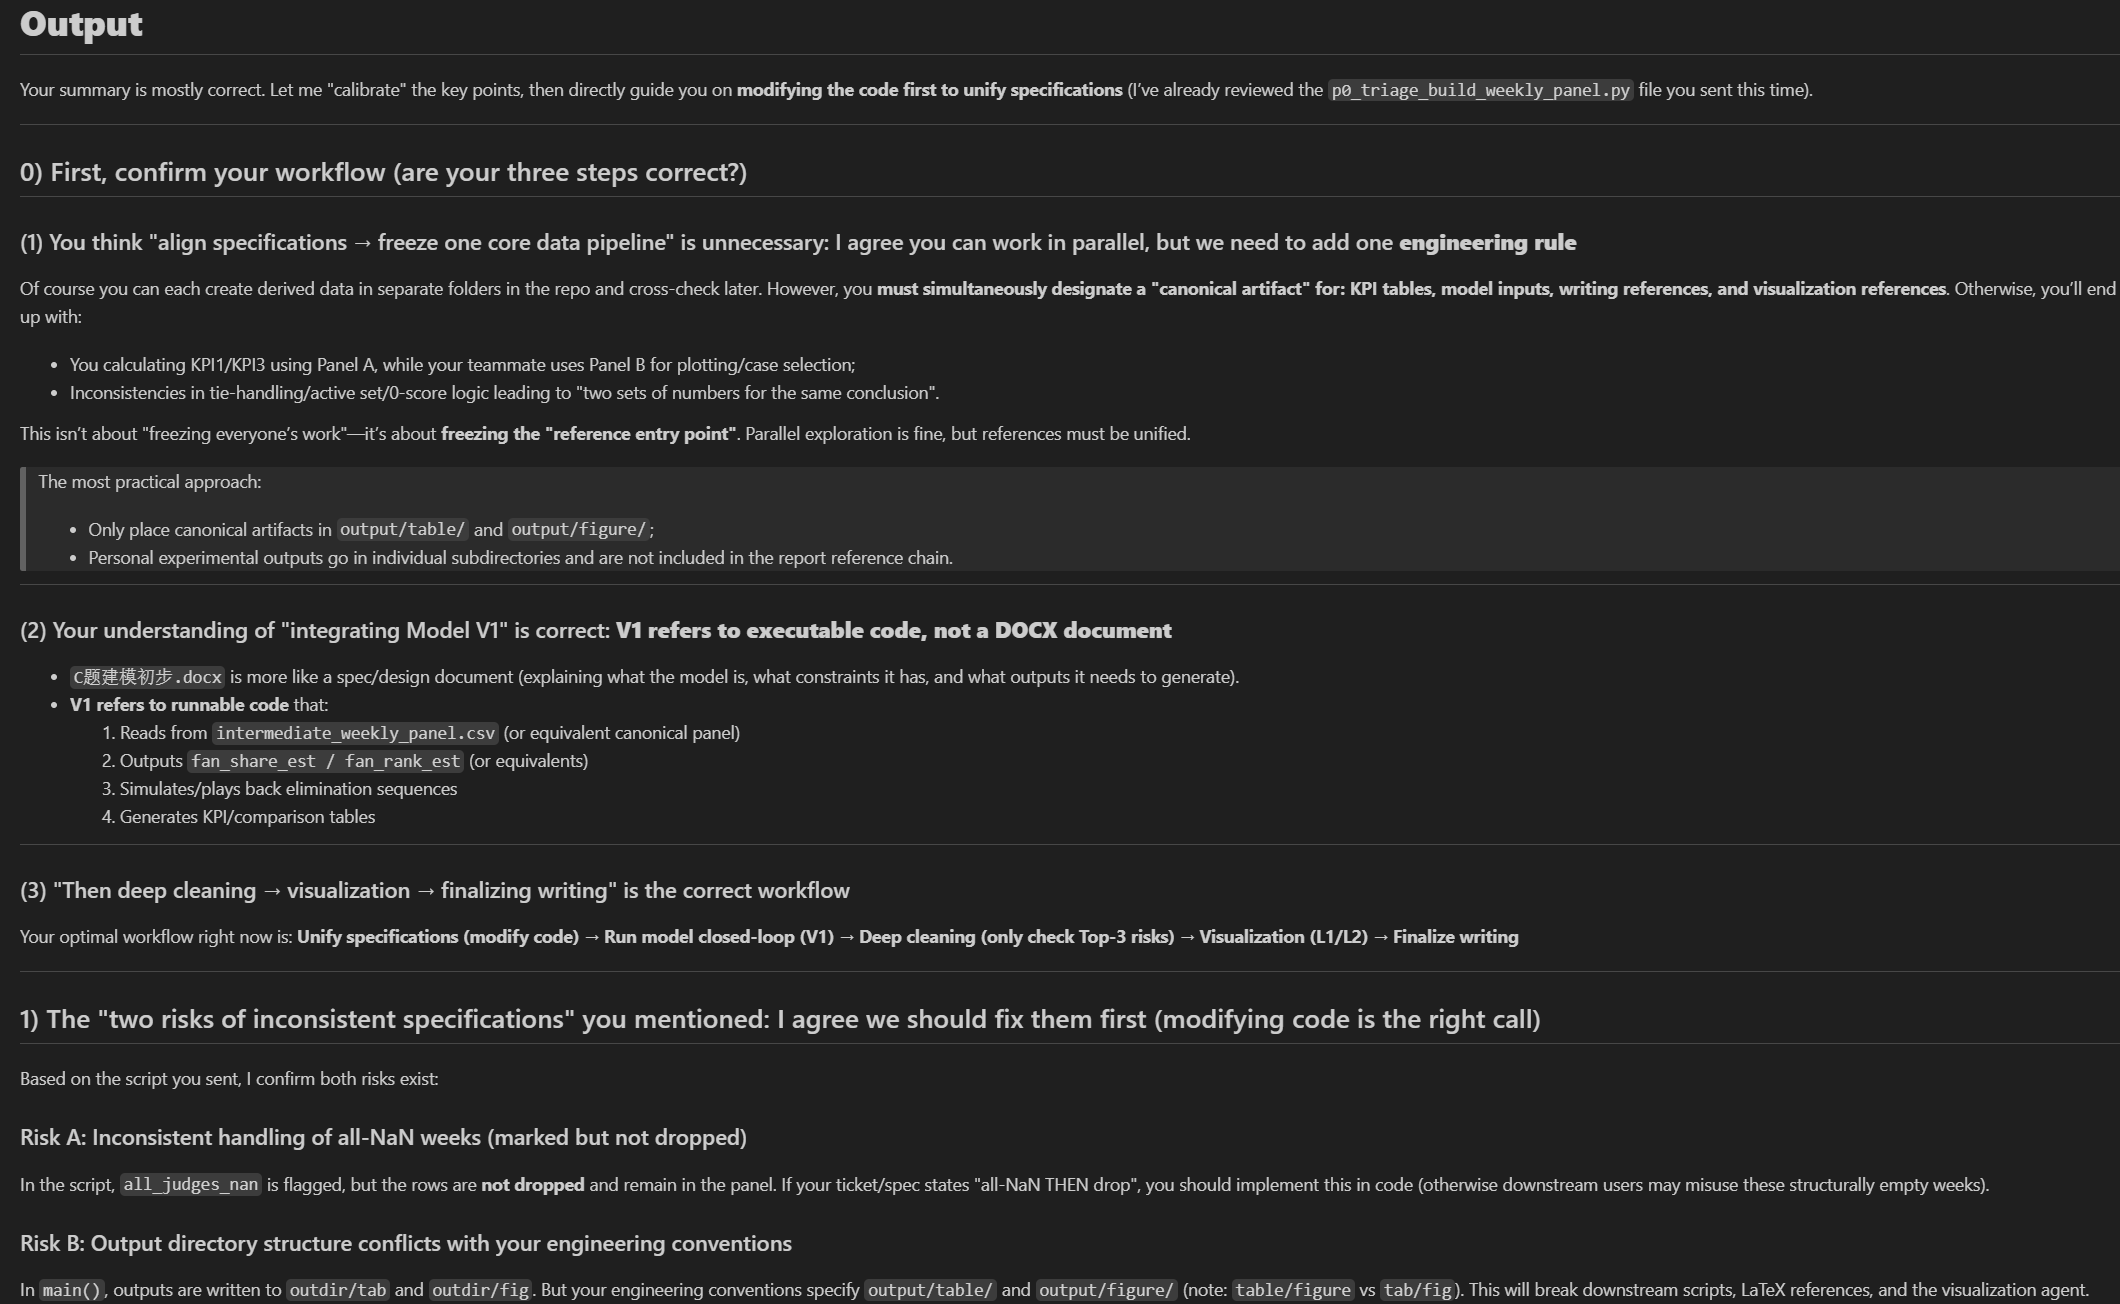
\includegraphics[width=0.9\linewidth]{report_on_use_of_ai/pho/131.png}
  \caption{ChatGPT Query 13 Output Screenshot}
  \label{fig:chatgpt_query_13_output}
\end{figure}
\begin{figure}
  \centering
  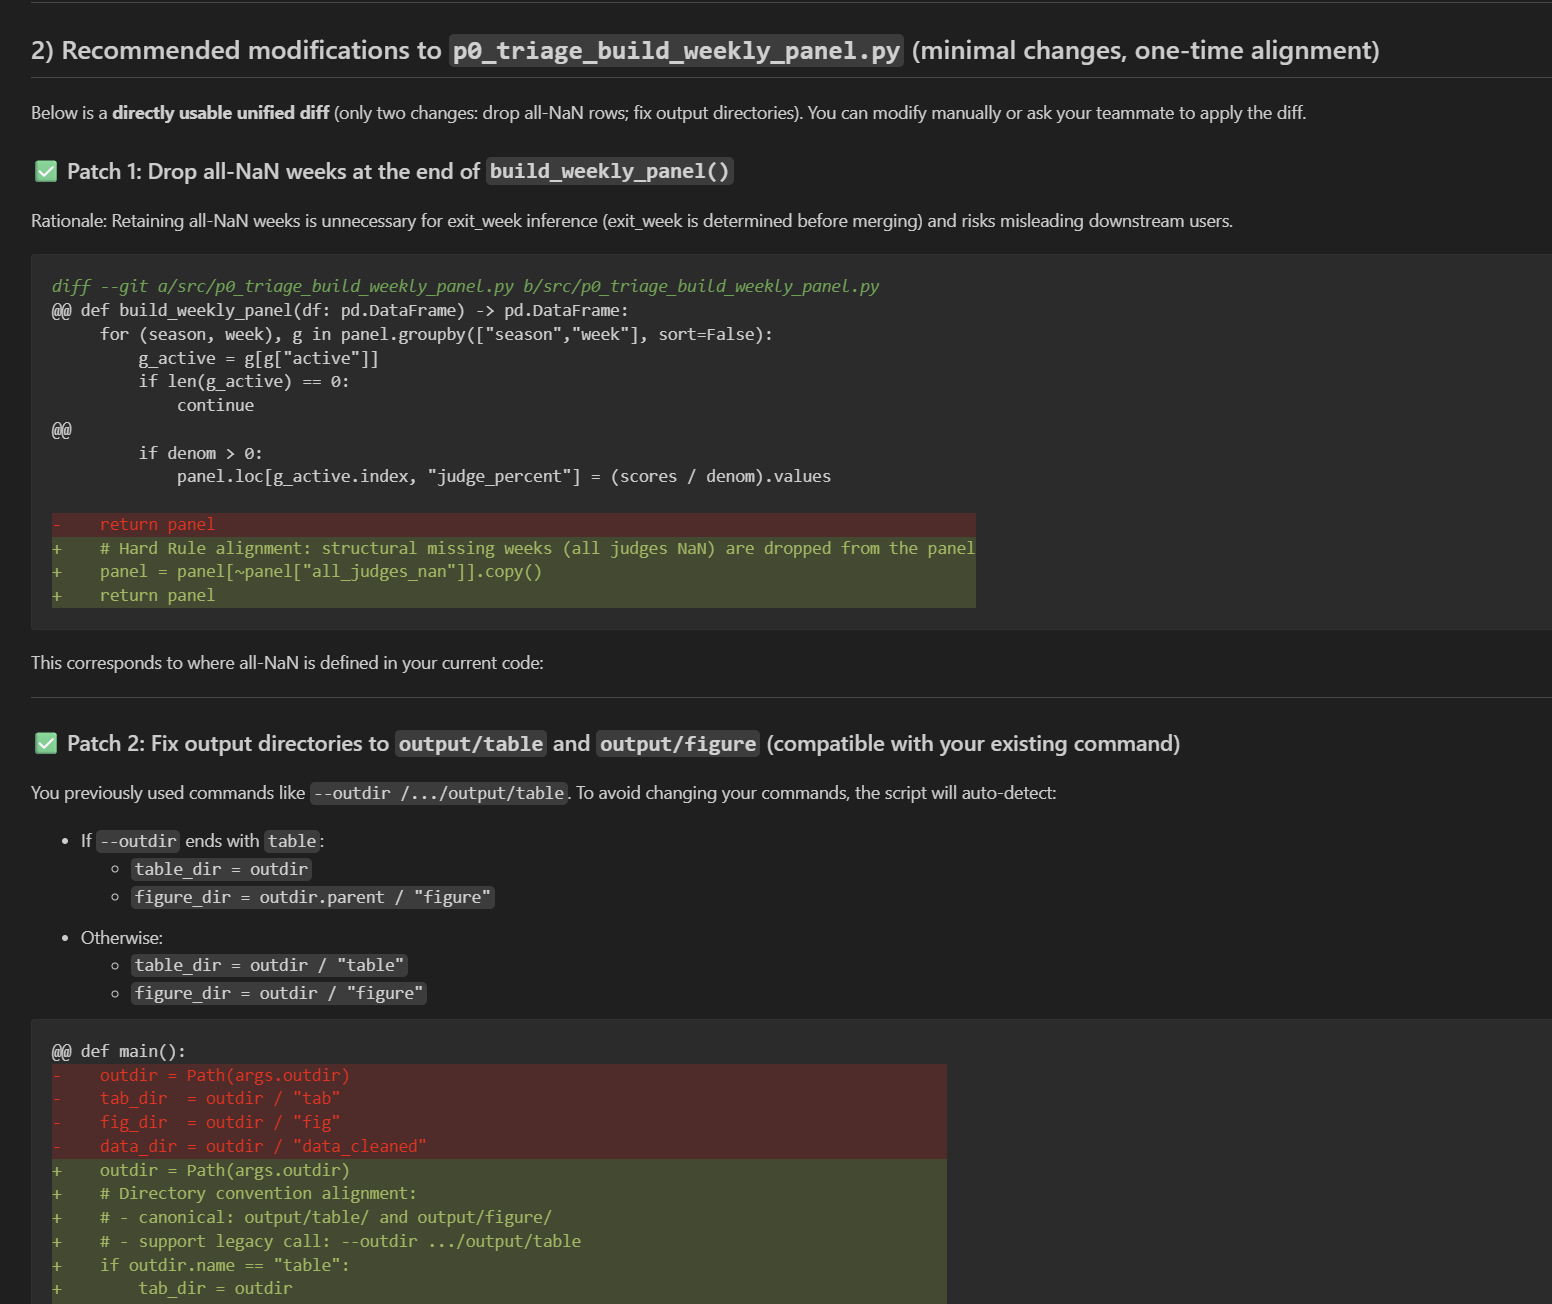
\includegraphics[width=0.9\linewidth]{report_on_use_of_ai/pho/132.png}
  \caption{ChatGPT Query 13 Output Screenshot}
  \label{fig:chatgpt_query_13_output_1}
\end{figure}
\begin{figure}
  \centering
  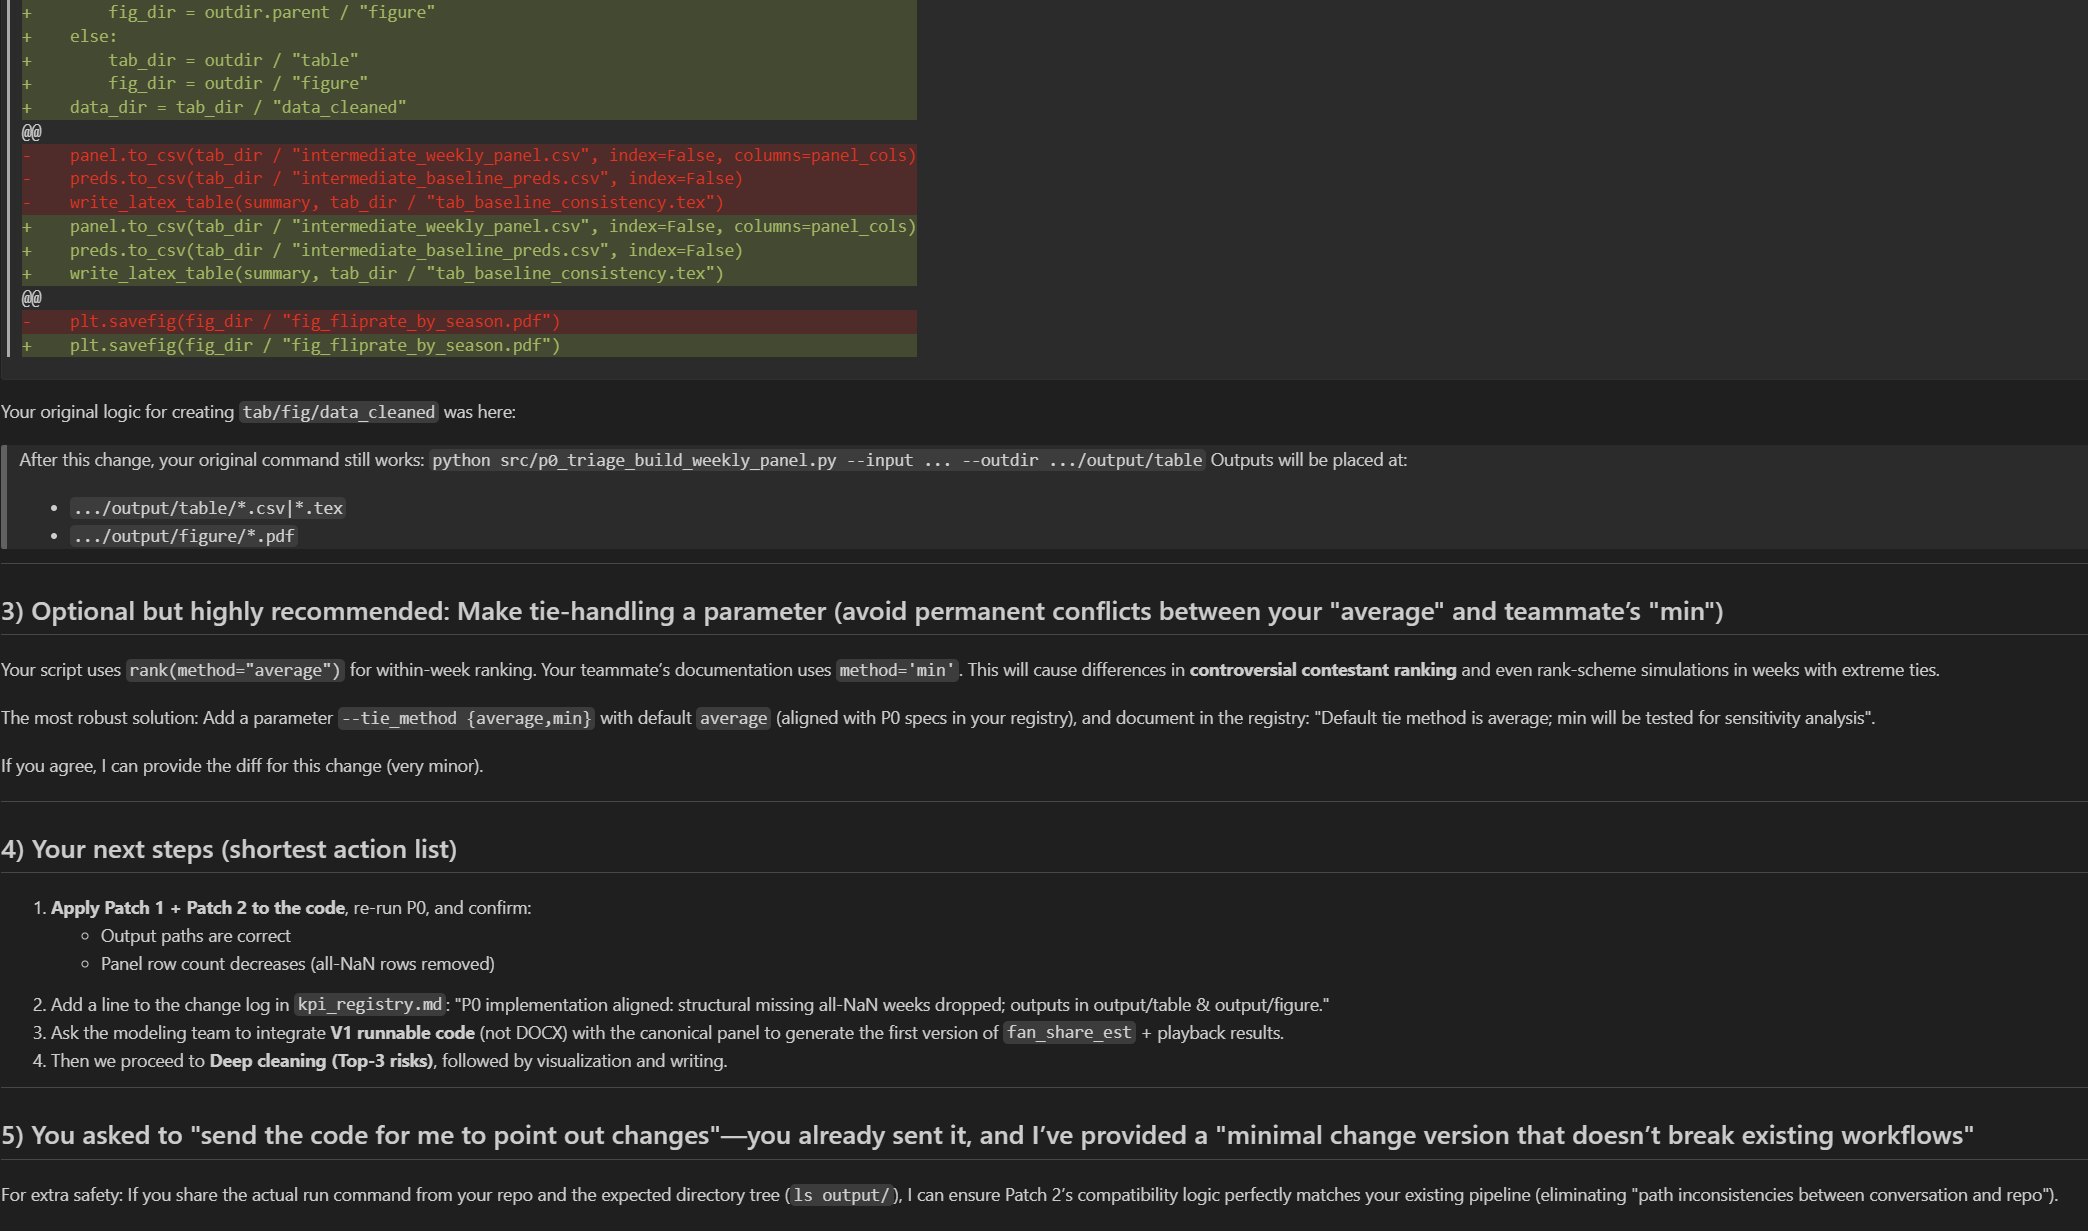
\includegraphics[width=0.9\linewidth]{report_on_use_of_ai/pho/133.png}
  \caption{ChatGPT Query 13 Output Screenshot}
  \label{fig:chatgpt_query_13_output_2}
\end{figure}




\textbf{\href{https://github.com/charles65536/model2026-2/blob/main/report_on_use_of_ai/chatgpt_14_input_and_output.md}{ChatGPT Query 14:}}\\
\textbf{Input:}
No rush, let's first sort out what we currently have:\\
1. We have the complete problem statement.\\
2. We have the preliminary data produced by our data team member just now.\\
3. We have the preliminary model developed by our modeling team member.\\
Please let me know what other files are needed and I will provide them.

Therefore, I think our workflow should be as follows:\\
1. First, complete the construction of the framework.\\
2. Then, provide you with our modeling spec, and then see which parts we can complete (my initial idea is that we can first finish the "Problem Restatement", "Key Assumptions", "Core Variables", and a bit of the beginning of the model; please supplement anything that is missing).\\
3. We will investigate the existing files and write the parts that can be included in the article.\\
\textbf{Output:}
\begin{figure}[H]
  \centering
  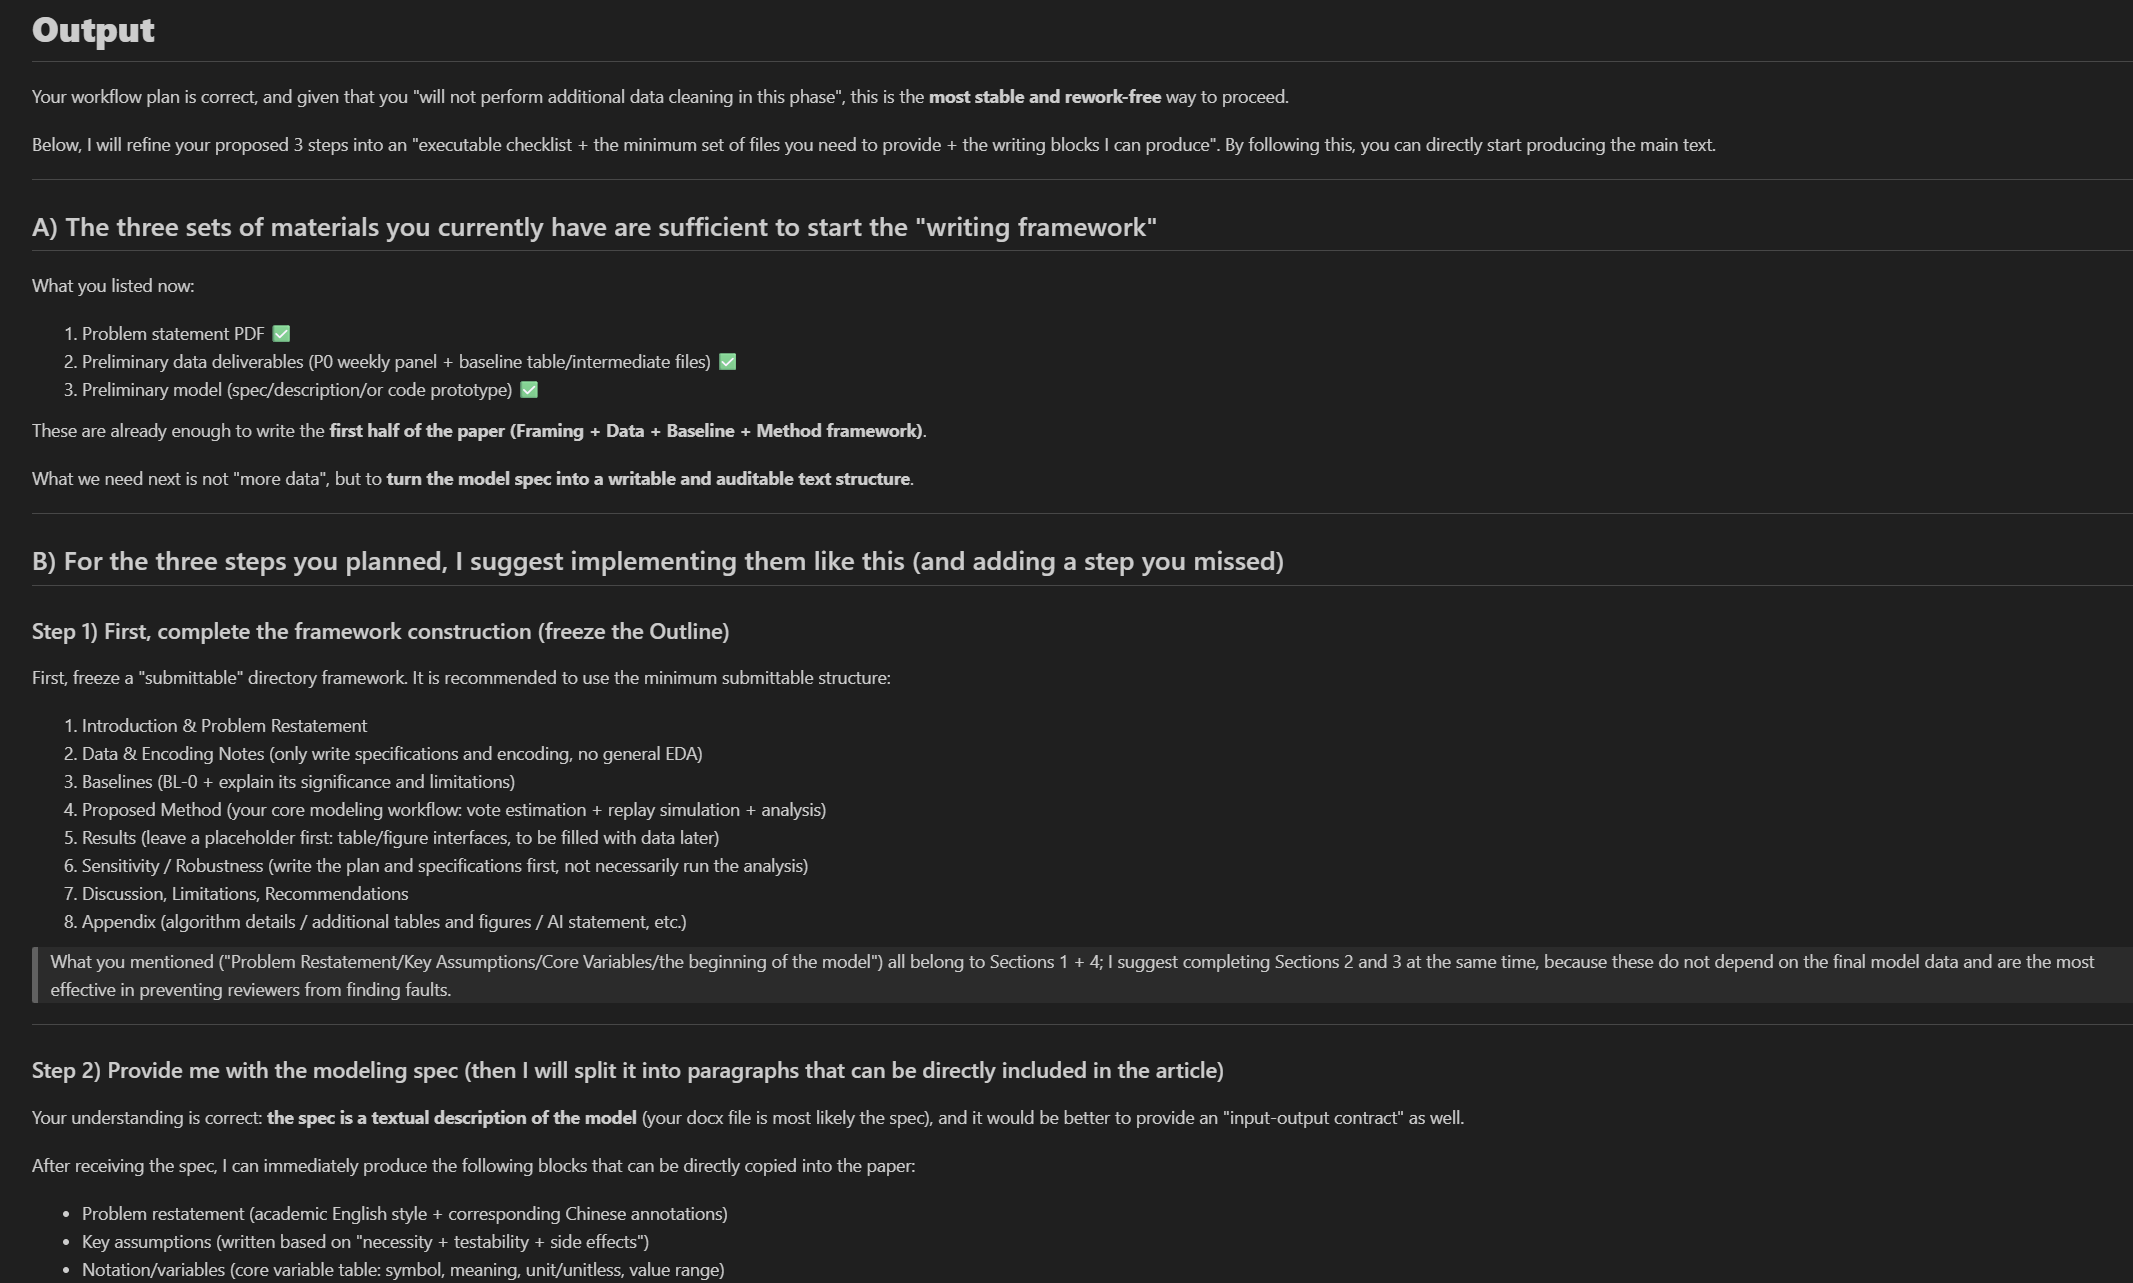
\includegraphics[width=0.9\linewidth]{report_on_use_of_ai/pho/141.png}
  \caption{ChatGPT Query 14 Output Screenshot}
  \label{fig:chatgpt_query_14_output}
\end{figure}
\begin{figure}[H]
  \centering
  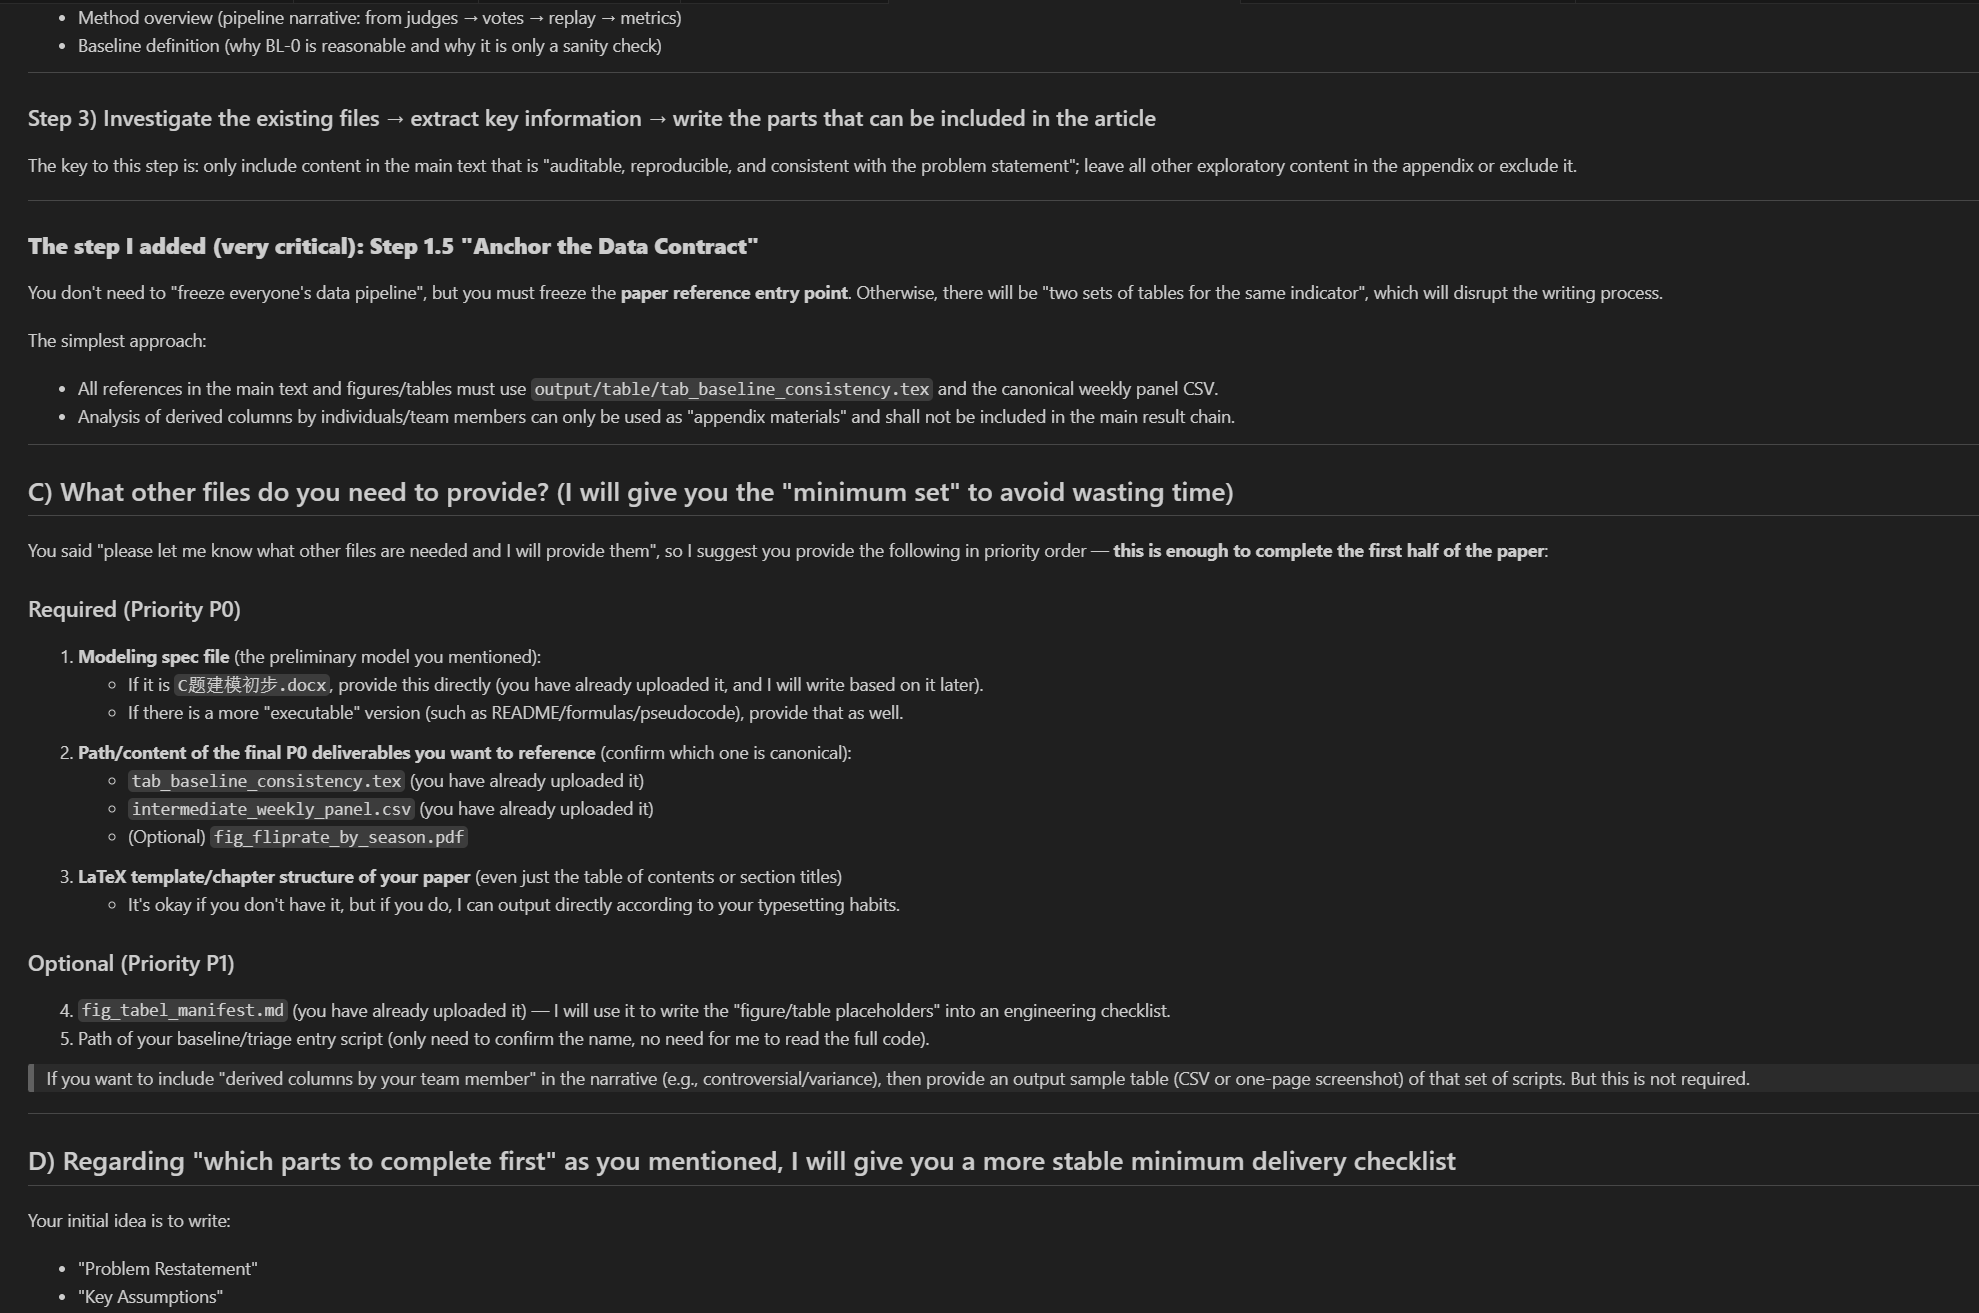
\includegraphics[width=0.9\linewidth]{report_on_use_of_ai/pho/142.png}
  \caption{ChatGPT Query 14 Output Screenshot}
  \label{fig:chatgpt_query_14_output_1}
\end{figure}
\begin{figure}[H]
  \centering
  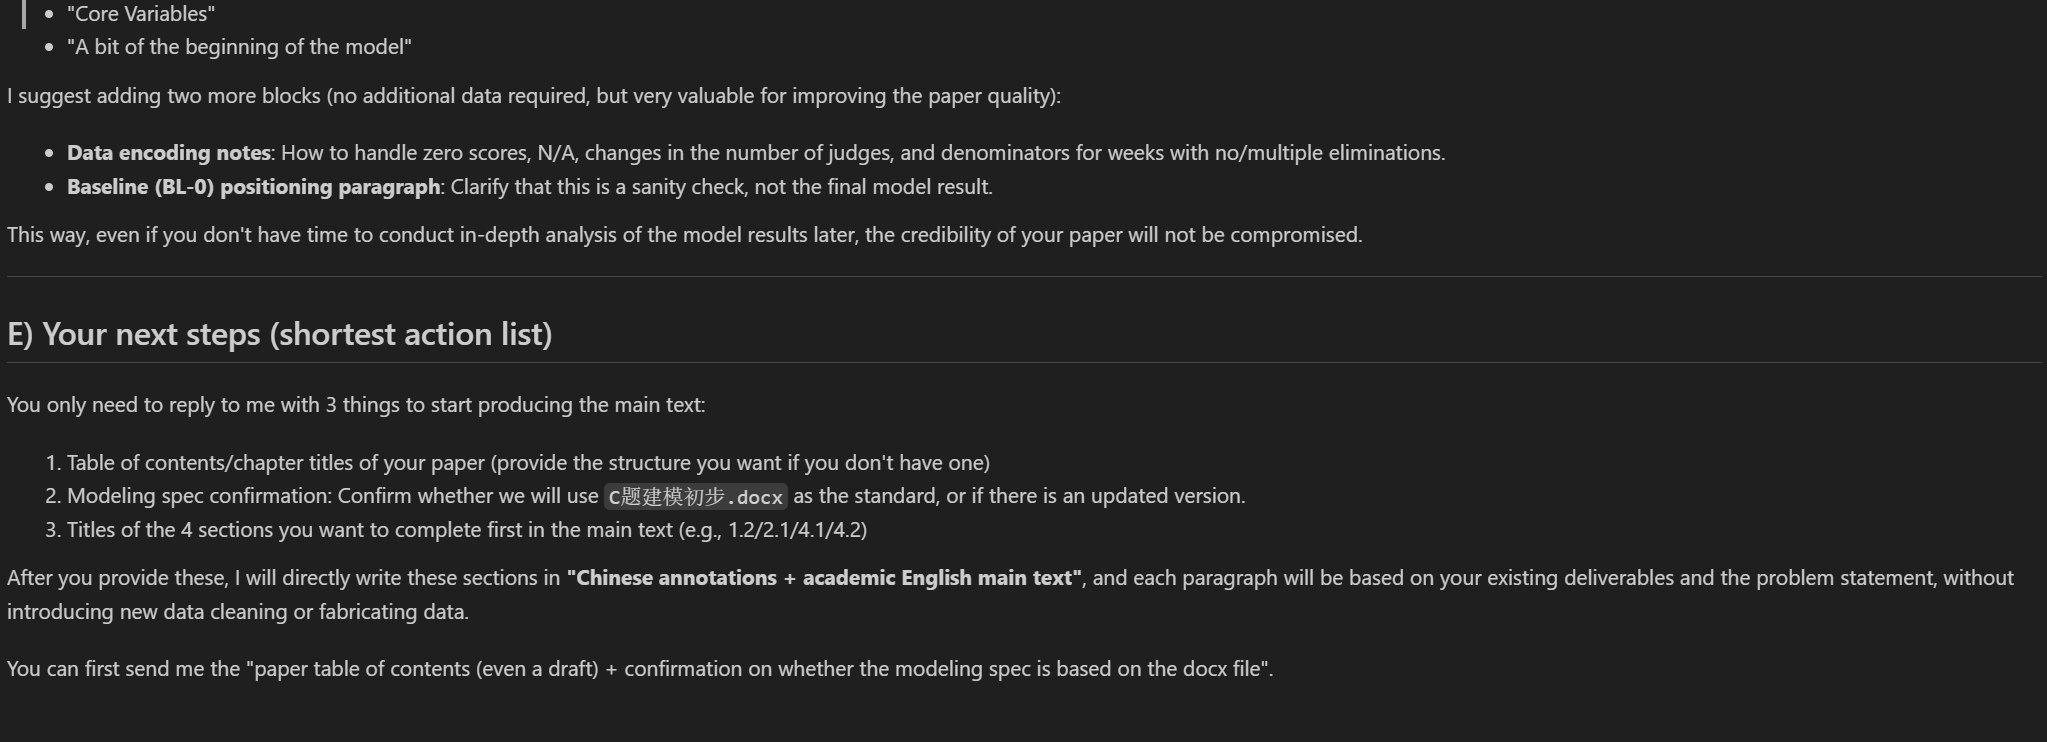
\includegraphics[width=0.9\linewidth]{report_on_use_of_ai/pho/143.png}
  \caption{ChatGPT Query 14 Output Screenshot}
  \label{fig:chatgpt_query_14_output_2}
\end{figure}



\subsection*{\center{Human Contribution Declaration}}
We affirm that:
\begin{enumerate}
  \item All final modeling decisions, algorithm designs, and strategic choices were made by the team members.
  \item All mathematical formulations and assumptions were independently derived or verified by the team.
  \item All code included in this project was reviewed, tested, and fully understood by the team.
  \item AI tools were used only for brainstorming, drafting, language refinement, and preliminary coding assistance.
  \item The submitted work represents our own understanding and intellectual contribution.
\end{enumerate}
\begin{flushright}
Date: Feb 2, 2026
\end{flushright}
\normalsize